\documentclass[table,aspectratio=169]{beamer}
%% Choose aspect ratio:
% [aspectratio=43]  % 4:3 (default)
% [aspectratio=169] % 16:9, wide

\usetheme[minimal, nofont, noheadline]{tugraz2018}
% \usetheme[iaik,]{tugraz2018}
%% Choose main theme variant:
% [standard]        % standard (default)
% [iaik]       % with institute's graphical acronym on the left
% [minimal]         % with reduced visuals

%% Choose your font style:
%                   % Helvetica (default for Corporate Design)
% [webfont]         % Source Sans Pro (as used on tugraz.at)
% [nofont]          % no font loaded - Computer Modern Sans

%% Choose your department's color instead of TU Graz tugred (optional):
% [arch]            % 
% [bau]             %
% [etit]            %
% [mbww]            %
% [tcvp]            %
% [mpug]            %
% [infbio]          %


\usepackage[utf8]{inputenc}
\usepackage[english]{babel}
%% Choose your language:
% [ngerman]   % German
% [english]   % English


%% Add your own packages, macros, etc.
\usepackage{xcolor, colortbl}
\usepackage{mathtools}
\usepackage{booktabs,nicematrix}
\usepackage{rotating}
\usepackage{listings}
\usepackage[style=alphabetic,backend=biber]{biblatex} % Bibliography
\addbibresource{\jobname.bib}                         % Bibliography
\usepackage{fontawesome}
\usepackage{filecontents}
\usepackage{mathrsfs}
\usepackage{amsmath}
\usepackage{setspace}
\usepackage{subcaption}
\usepackage{multirow}
\usepackage{bm}
\usepackage{pgfplots}
\usepackage[linesnumbered,ruled,vlined]{algorithm2e}
\usepackage{framed, color}

\usepackage{tikz}
\usepgfplotslibrary{external} % Library for externalization
\usetikzlibrary{calc, patterns, cipher, arrows.meta, shapes.geometric, positioning, decorations.pathreplacing, decorations.markings, decorations.pathmorphing}
\usepackage{skinny}
\usepackage{tugcolors}
\usepackage{skinnyzero} % definitions for figures: colors, etc
\setbeamersize
{
	text margin left=0.4cm,
	text margin right=0.4cm
}

%% Enter presentation metadata
\title{Improved Search for Integral, Impossible Differential and Zero-Correlation Attacks}
\author{\underline{\textbf{Hosein Hadipour}} \and Simon Gerhalter \and Sadegh Sadeghi \and Maria Eichlseder}
\date{FSE 2024 - Leuven, Belgium}
%\institute{IAIK}
\instituteurl{hsn.hadipour@gmail.com}

%% Logos
%\institutelogo{beamerthemetugraz/institute/IAIK}  % graphical acronym for [] theme (left margin)
% \additionallogo{figures/logo}  % additional institute/department logo (footline; optional)
% \logobar{Supported by: ...}  % sponsors (titlepage; optional)

%% Macros
\newcommand{\tikzmark}[1]{\tikz[overlay,remember picture] \node (#1) {};}
\newcommand{\pstabstyle}{\small\renewcommand{\tabcolsep}{3pt}}
%\newcommand{\KeysData}{Keys & Data}
%\newcommand{\KeysData}{\multicolumn{2}{c}{K $\times$ D}}
\newcommand{\KeysData}{K & D}

\newcommand{\smallmath}{\everydisplay{\fontsize{8pt}{10pt}\selectfont}}

%%% commands to represent CSP/COP variables/constraints%%%
\newcommand{\ax}{\texttt{AX}\xspace} %AX
\newcommand{\ay}{\texttt{AY}\xspace} %AY
\newcommand{\az}{\texttt{AZ}\xspace} %AZ
\newcommand{\dx}{\texttt{DX}\xspace} %DX
\newcommand{\dy}{\texttt{DY}\xspace} %DY
\newcommand{\dz}{\texttt{DZ}\xspace} %DZ

\newcommand{\axu}{\texttt{AXU}\xspace} %AXU
\newcommand{\ayu}{\texttt{AYU}\xspace} %AYU
\newcommand{\azu}{\texttt{AZU}\xspace} %AZU
\newcommand{\dxu}{\texttt{DXU}\xspace} %DXU
\newcommand{\dyu}{\texttt{DYU}\xspace} %DYU
\newcommand{\dzu}{\texttt{DZU}\xspace} %DZU
\newcommand{\lxu}{\texttt{LXU}\xspace} %LXU
\newcommand{\axl}{\texttt{AXL}\xspace} %AXL
\newcommand{\ayl}{\texttt{AYL}\xspace} %AYL
\newcommand{\azl}{\texttt{AZL}\xspace} %AZL
\newcommand{\dxl}{\texttt{DXL}\xspace} %DXL
\newcommand{\dyl}{\texttt{DYL}\xspace} %DYL
\newcommand{\dzl}{\texttt{DZL}\xspace} %DZL
\newcommand{\lxl}{\texttt{LXL}\xspace} %LXL
\newcommand{\astk}{\texttt{ASTK}\xspace} %ASTK

\newcommand{\D}{\texttt{D}\xspace} %Data complexity D[0], D[1]
\newcommand{\T}{\texttt{T}\xspace} %Time complexity T[0], T[1], T[2], T[3]
\newcommand{\W}{\texttt{W}\xspace} %hamming weight of IO differences
\newcommand{\C}{\texttt{C}\xspace} %c parameters c\In, c\Out
\newcommand{\s}{\texttt{c}\xspace} %s: cell size in our CP formulas
\newcommand{\z}{\texttt{z}\xspace} %z: number of tweakey paths in SKINNY

\newcommand{\cp}[1]{\textit{\texttt{#1}}\xspace} % CP x
\newcommand{\csp}{\textit{\texttt{CSP}}\xspace} % CSP problem
\newcommand{\cop}{\textit{\texttt{COP}}\xspace} % COP problem
\newcommand{\cpmodel}{\mathcal{M}\xspace} % CP model M
\newcommand{\cpvars}{\mathcal{M}.\texttt{var}\xspace} % CP variables
\newcommand{\cpcons}{\mathcal{M}.\texttt{con}\xspace} % CP constraints
\newcommand{\cpobj}{\mathcal{M}.\texttt{obj}\xspace} % CP objective
\newcommand{\booltoint}{\textit{\texttt{bool2int}}\xspace} % CP bool2int operator
\newcommand{\cpif}{\textit{\texttt{if}}\xspace} % CP If
\newcommand{\cpthen}{\textit{\texttt{then}}\xspace} % CP Then
\newcommand{\cpelse}{\textit{\texttt{else}}\xspace} % CP Else
\newcommand{\cpelseif}{\textit{\texttt{elseif}}\xspace} % CP Elseif
\newcommand{\cpendif}{\textit{\texttt{endif}}\xspace} % CP Endif

\newcommand{\cplink}{\textit{\texttt{Link}}\xspace} % CP Link
\newcommand{\cpxor}{\textit{\texttt{XOR}}\xspace} % CP XOR
\newcommand{\cpsbox}{\textit{\texttt{S-box}}\xspace} % CP S-box
\newcommand{\cpbranch}{\textit{\texttt{Branch}}\xspace} % CP Branching
\newcommand{\cpcopy}{\textit{\texttt{Copy}}\xspace} % Copy: equivalent to branching point
\newcommand{\cptrue}{\textit{\texttt{True}}\xspace} % CP True
\newcommand{\cpfalse}{\textit{\texttt{False}}\xspace} % CP False
\newcommand{\cpmin}{\textit{\texttt{min}}\xspace} % CP Min
\newcommand{\cpmdiff}{\textit{\texttt{Mdiff}}\xspace} % CP Mdiff
\newcommand{\cpminvdiff}{\textit{\texttt{Minvdiff}}\xspace} % CP Minvdiff

% notation for ID and figures
\newcommand{\In}{_{\textsc{b}}} % input difference of Ei (initial key-recovery rounds)
\newcommand{\Out}{_{\textsc{f}}} % output difference of Eo (final key-recovery rounds)
\newcommand{\Up}{_{\textsc{u}}} % input difference of Eu (initial distinguisher rounds)
\newcommand{\Low}{_{\textsc{l}}} % output difference of El (final distinguisher rounds)
\newcommand{\Dist}{_{\textsc{d}}} % distinguisher rounds Eu, El (middle)
\newcommand{\KB}{_{\textsc{KB}}} % Key-Bridging
\newcommand{\GD}{_{\textsc{GD}}} % Guess-and-Determine
\newcommand{\DP}{_{\textsc{DP}}} % Difference Propagation
\newcommand{\Off}{_{\text{off}}} % offset for round counter in Eu, El, and Ef
\newcommand{\Tot}{_\textit{Tot}}
\newcommand{\STK}{\textit{STK}}
\newcommand{\ETK}{\textit{ETK}}
\newcommand{\TK}{\textit{TK}}
\newcommand{\lane}{\textit{Lane}}
\newcommand{\cs}{c} % indicates the cell size in the main body
\newcommand{\as}{m} % indicates the state array size in the main body
\newcommand{\Rinit}{\textbf{r}_{\textbf{i}}} % Rinit for ForkSKINNY: the number of rounds before fork
\newcommand{\Rzero}{\textbf{r}_{\textsc{0}}} % R0 for ForkSKINNY: the length of C0 branch
\newcommand{\Rone}{\textbf{r}_{\textsc{1}}} % R1 for ForkSKINNY: the length of C1 branch
\newcommand{\bis}{\text{--}}

%%% format of the codes %%%
\lstdefinelanguage{Sage}[]{Python}{morekeywords={True,False,sage,cdef,cpdef,ctypedef,self, elseif, endif},sensitive=true}

\lstdefinestyle{mystyle}{
  backgroundcolor=\color{backcolour},
  commentstyle=\color{codegreen},
  keywordstyle={\color{magenta}\bfseries},
  numberstyle=\tiny\color{codegray},
  stringstyle=\color{codepurple},
  basicstyle=\ttfamily\footnotesize,
  breakatwhitespace=false,
  breaklines=true,
  captionpos=b,
  keepspaces=true,
  numbers=left,
  numbersep=5pt,
  showspaces=false,
  showstringspaces=false,
  showtabs=false,
  tabsize=2
}
\lstset{style=mystyle, language=Sage}
\definecolor{codegreen}{rgb}{0,0.6,0}
\definecolor{codegray}{rgb}{0.5,0.5,0.5}
\definecolor{codepurple}{rgb}{0.58,0,0.82}
\definecolor{backcolour}{rgb}{0.95,0.95,0.92}

\makeatletter
\NewDocumentCommand{\DrawBox}{s O{}}{%
    \tikz[overlay,remember picture]{
    \IfBooleanTF{#1}{%
        \coordinate (RightPoint) at ($(left |- right)+(\linewidth-\labelsep-\labelwidth,0.0)$);
    }{%
        \coordinate (RightPoint) at (right.east);
    }%
    \draw[red,#2]
      ($(left)+(-0.2em,0.9em)$) rectangle
      ($(RightPoint)+(0.2em,-0.3em)$);}
}

\NewDocumentCommand{\DrawBoxWide}{s O{}}{%
    \tikz[overlay,remember picture]{
    \IfBooleanTF{#1}{%
        \coordinate (RightPoint) at ($(left |- right)+(\linewidth-\labelsep-\labelwidth,0.0)$);
    }{%
        \coordinate (RightPoint) at (right.east);
    }%
    \draw[red,#2]
      ($(left)+(-\labelwidth,0.9em)$) rectangle
      ($(RightPoint)+(0.2em,-0.3em)$);}
}

\def\rowcolor{\noalign{\ifnum0=`}\fi\bmr@rowcolor}
\newcommand<>{\bmr@rowcolor}{%
    \alt#1%
        {\global\let\CT@do@color\CT@@do@color\@ifnextchar[\CT@rowa\CT@rowb}% 
        {\ifnum0=`{\fi}\@gooble@rowcolor}% 
}
\newcommand{\@gooble@rowcolor}[2][]{\@gooble@rowcolor@}
\newcommand{\@gooble@rowcolor@}[1][]{\@gooble@rowcolor@@}
\newcommand{\@gooble@rowcolor@@}[1][]{\ignorespaces}

%%%%%%%%%%%%%%%%%%%%%%%%%%%%%%%%%%%%%%%%%%%%%%%%%%%%%%%%%%%%%%%%%%%%%%%%
% For Partial-sum example on AES
\colorlet{act}{tugyellow}
\colorlet{con}{white}
\colorlet{bal}{colB}
\newcommand{\PSfont}{\footnotesize}
\newcommand{\PScale}{.88}
\newcommand{\iAct}[1]{\Fill[act]{#1}\Cell{#1}{\color{white}\PSfont A}}
\newcommand{\iBal}[1]{\Fill[bal]{#1}\Cell{#1}{\color{white}\PSfont B}}
\newcommand{\iCon}[1]{\Fill[con]{#1}\Cell{#1}{\color{gray}\PSfont C}}
\newcommand{\iStep}[2]{\Fill[tugblue]{#1}\Cell{#1}{\color{white}\PSfont\texttt #2}}
\newcommand{\iKey}[2]{\Fill[tuggreen]{#1}\Cell{#1}{\color{white}\PSfont\texttt #2}}
\newcommand{\iPartial}[2]{\Fill[tugyellow]{#1}\Cell{#1}{\color{white}\PSfont\texttt #2}}

\newcommand{\SingleCell}[1]{
  \tikz[stateopts]{ %, rounded corners=2pt
    \draw (.5,-.5) coordinate (s);
    #1
  }  
}

\newcommand{\PartialSumStepInit}{
  \tikz[yscale=\PScale]{
    \foreach \i/\s in {0/1,1/1,2/2,3/3} {
      \ifcase \i
        \draw ++(\i*.5+1,0) node[inner sep=0pt] (c\i) {\SingleCell{\iStep{s}{\s}}};
      \or
        \draw ++(\i*.5+1,0) node[inner sep=0pt] (c\i) {\SingleCell{\iStep{s}{\s}}};
      \else
        \draw ++(\i*.5+1,0) node[inner sep=0pt, opacity=0.5] (c\i) {\SingleCell{\iStep{s}{\s}}};
      \fi
    }

    \foreach \i/\in/\s in {0/0/1,1/1/1} {
      \draw (c\in) ++(0,-.5-\i*.35) coordinate[xor] (xorc\i);
      \draw (c0) ++(-\in*.5-.5, 0) node[inner sep=0pt] (k\i) {\SingleCell{\iKey{s}{\s}}};
      \draw (c\in.south) ++(0,-1.3) node[sbox,inner sep=2pt] (sbox\in) {$\mathcal{S}_{\i}$};

      \draw[->, rounded corners=2pt] (c\in.south) -- (xorc\in.north);
      \draw[->, rounded corners=2pt] (k\in.south) |- (xorc\in.west);

      \draw[->, rounded corners=2pt] (xorc\in) -- (sbox\in);
    }

    \draw (sbox1) ++(0,-.5) coordinate[xor] (xors);

    \draw[->, rounded corners=2pt] (sbox1) -- (xors);
    \draw[->, rounded corners=2pt] (sbox0) |- (xors);

    \draw (c2 |- xors) ++(0,-.5) node[sbox, minimum width=3.0cm, inner sep=2pt] (count) {\texttt{count}};

    \draw[->, rounded corners=2pt] (xors.south) -- (xors |- count.north);
    \draw[->, rounded corners=2pt] (c2.south) -- (c2 |- count.north);
    \draw[->, rounded corners=2pt] (c3.south) -- (c3 |- count.north);

    \draw[->, rounded corners=2pt] (xors |- count.south) -- ++(0,-.2);
    \draw[->, rounded corners=2pt] (c2 |- count.south) -- ++(0,-.2);
    \draw[->, rounded corners=2pt] (c3 |- count.south) -- ++(0,-.2);
  }
}

\newcommand{\PartialSumStepTwo}{
  \tikz[yscale=\PScale]{
    \draw node[inner sep=0pt, opacity=0.5] (k1) {\SingleCell{\iKey{s}{1}}}
    ++(.5, 0) node[inner sep=0pt, opacity=0.5] (k2) {\SingleCell{\iKey{s}{1}}}
    ++(.5, 0) node[inner sep=0pt] (k) {\SingleCell{\iKey{s}{2}}}
    ++(.5,0) node[inner sep=0pt] (c1) {\SingleCell{\iPartial{s}{2}}}
    ++(.5,0) node[inner sep=0pt] (c2) {\SingleCell{\iStep{s}{2}}}
    ++(.5,0) node[inner sep=0pt, opacity=0.5] (c3) {\SingleCell{\iStep{s}{3}}};


    \draw (c2) ++(0,-.5) coordinate[xor] (xorc);

    \draw (c2.south) ++(0,-.8) node[sbox,inner sep=2pt] (sbox) {$\mathcal{S}_{2}$};

    \draw[->, rounded corners=2pt] (c2.south) -- (xorc.north);
    \draw[->, rounded corners=2pt] (k.south) |- (xorc.west);

    \draw[->, rounded corners=2pt] (xorc) -- (sbox);

    \draw (sbox) ++(0,-.5) coordinate[xor] (xors);

    \draw[->, rounded corners=2pt] (sbox) -- (xors);
    \draw[->, rounded corners=2pt] (c2.south) ++(-.5,0) -- ++(0,-1.3) -- (xors);

    \draw (c2 |- xors) ++(.25,-.5) node[sbox, minimum width=2.15cm, inner sep=2pt] (count) {\texttt{count}};

    \draw[->, rounded corners=2pt] (xors.south) -- (xors |- count.north);
    \draw[->, rounded corners=2pt] (c3.south) -- (c3 |- count.north);

    \draw[->, rounded corners=2pt] (xors |- count.south) -- ++(0,-.2);
    \draw[->, rounded corners=2pt] (c3 |- count.south) -- ++(0,-.2);
  }  
}

\newcommand{\PartialSumStepThree}{
  \tikz[yscale=\PScale]{
    \draw node[inner sep=0pt, opacity=0.5] (k1) {\SingleCell{\iKey{s}{1}}}
    ++(.5, 0) node[inner sep=0pt, opacity=0.5] (k2) {\SingleCell{\iKey{s}{1}}}
    ++(.5, 0) node[inner sep=0pt, opacity=0.5] (k3) {\SingleCell{\iKey{s}{2}}}
    ++(.5, 0) node[inner sep=0pt] (k) {\SingleCell{\iKey{s}{3}}}
    ++(.5,0) node[inner sep=0pt] (c1) {\SingleCell{\iPartial{s}{3}}}
    ++(.5,0) node[inner sep=0pt] (c2) {\SingleCell{\iStep{s}{3}}};

    \draw (c2) ++(0,-.5) coordinate[xor] (xorc);

    \draw (c2.south) ++(0,-.8) node[sbox,inner sep=2pt] (sbox) {$\mathcal{S}_{3}$};

    \draw[->, rounded corners=2pt] (c2.south) -- (xorc.north);
    \draw[->, rounded corners=2pt] (k.south) |- (xorc.west);

    \draw[->, rounded corners=2pt] (xorc) -- (sbox);

    \draw (sbox) ++(0,-.5) coordinate[xor] (xors);

    \draw[->, rounded corners=2pt] (sbox) -- (xors);
    \draw[->, rounded corners=2pt] (c2.south) ++(-.5,0) -- ++(0,-1.3) -- (xors);

    \draw (xors) ++(0,-.5) node[sbox, minimum width=1.3cm, inner sep=2pt] (count) {\texttt{count}};

    \draw[->, rounded corners=2pt] (xors.south) -- (xors |- count.north);

    \draw[->, rounded corners=2pt] (xors |- count.south) -- ++(0,-.2);
  }  
}

\newcommand{\PartialSumStepFinal}{
  \tikz[remember picture,yscale=\PScale]{
    \draw node[inner sep=0pt, opacity=0.5] (k1) {\SingleCell{\iKey{s}{1}}}
    ++(.5, 0) node[inner sep=0pt, opacity=0.5] (k2) {\SingleCell{\iKey{s}{1}}}
    ++(.5, 0) node[inner sep=0pt, opacity=0.5] (k3) {\SingleCell{\iKey{s}{2}}}
    ++(.5, 0) node[inner sep=0pt, opacity=0.5] (k3) {\SingleCell{\iKey{s}{3}}}
    ++(.5, 0) node[inner sep=0pt] (k) {\SingleCell{\iKey{s}{4}}}
    ++(.5,0) node[inner sep=0pt] (c) {\SingleCell{\iPartial{s}{4}}};

    \draw (c) ++(0,-.5) coordinate[xor] (xorc);
    \draw (c.south) ++(0,-.8) node[sbox, color=white, minimum width=1.3cm, inner sep=2pt] (dummy) {\texttt{count}};
    \draw (c.south) ++(0,-.8) node[sbox,inner sep=2pt] (sbox) {$\mathcal{S}^{-1}$};

    \draw[->, rounded corners=2pt] (c.south) -- (xorc.north);
    \draw[->, rounded corners=2pt] (k.south) |- (xorc.west);

    \draw[->, rounded corners=2pt] (xorc) -- (sbox);
  } 
}

%%%%%%%%%%%%%%%%%%%%%%%%%%%%%%%%%%%%%%%%%%%%%%%%%%%%%%%%%%%%%%%%%%%%%%%%
\newcommand{\sparen}{\vspace*{-.3cm}}
\makeatother


%%%%%%%%%%%%%%%%%%%%%%%%%%%%%%%%%%%%%%%%%%%%%%%%%%%%%%%%%%%%%%%%%%%%%%%%
%%%%%%%%%%%%%%%%%%%%%%%%%%%%%%%%%%%%%%%%%%%%%%%%%%%%%%%%%%%%%%%%%%%%%%%%
%%%%%%%%%%%%%%%%%%%%%%%%%%%%%%%%%%%%%%%%%%%%%%%%%%%%%%%%%%%%%%%%%%%%%%%%
\begin{document}
%%%%%%%%%%%%%%%%%%%%%%%%%%%%%%%%%%%%%%%%%%%%%%%%%%%%%%%%%%%%%%%%%%%%%%%%
\begin{frame}[plain]
  \maketitle
\end{frame}

%%%%%%%%%%%%%%%%%%%%%%%%%%%%%%%%%%%%%%%%%%%%%%%%%%%%%%%%%%%%%%%%%%%%%%%%
\begin{frame}{Motivation and Our Contributions}
  \begin{itemize}
    \small
    \item<1->[\faBinoculars] Motivation
    \begin{itemize}
      \item[\faCheckCircleO] Providing a tool to find \textbf{\textcolor{red}{complete}} integral, and ID/ZC attacks
    \end{itemize}
    \item<2->[\faDiamond] Contributions
    \begin{itemize}
      \item<2->[\faCheckCircle] Improving the CP-based methods to find ID/ZC, and integral distinguishers.
      \item<2->[\faCheckCircle] Introducing a CP model for the partial-sum technique for the first time.
      \item<2->[\faCheckCircle] Improving distinguishers of \cipher{Ascon}, \cipher{QARMAv2}, and \cipher{ForkSKINNY} (\textbf{25} Dists.).
      \item<2->[\faCheckCircle] Improving key recovery attacks of \cipher{SKINNY}, and \cipher{ForkSKINNY} (\textbf{24} Attacks).
    \end{itemize}
  \end{itemize}
  \end{frame}

%%%%%%%%%%%%%%%%%%%%%%%%%%%%%%%%%%%%%%%%%%%%%%%%%%%%%%%%%%%%%%%%%%%%%%%%
\begin{frame}{Part of Our Results Regarding Distinguishing Attacks}
\vspace{-0.6cm}
\begin{table}[h!]
  \centering\footnotesize
  \label{tab:summary_distinguishers}
  \begin{tabular}{@{}lllll@{}}
    \toprule
    Cipher & \#Rounds &  Dist. & Data complexity & Ref.\\
    \midrule
    \cipher{QARMAv2}-64 & 5 & Integral & - &  \cite{cryptoeprint_qarmav2}\\
    \cipher{QARMAv2}-64 ($\mathscr{T} = 1$) & \bf 7 / \bf 8 / \bf 9  & Integral & $\bf 2^{8}$ / $\bf 2^{16}$ / $\bf 2^{44}$ &  This work\\
    \cipher{QARMAv2}-64 ($\mathscr{T} = 2$) & \bf 8 / \bf 9 / \bf 10  & Integral & $\bf 2^{8}$ / $\bf 2^{16}$ / $\bf 2^{44}$ &  This work\\
    \cipher{QARMAv2}-128($\mathscr{T} = 2$) & \bf 10 / \bf 11 / \bf 12 & Integral & $\bf 2^{16}$ / $\bf 2^{44}$ / $2^{96}$ &  This work\\
    \midrule    
    \cipher{ForkSKINNY}-64-192  & 16 & Integral & $2^{72}$ &  \cite{ctrsa_NiuLSW21}\\
    \cipher{ForkSKINNY}-64-192 & \bf 17 & Integral & $\bf 2^{60}$ &  This work\\
    \cipher{ForkSKINNY}-64-192 & 16 & ID & - &  \cite{eurocrypt_HadipourSE23}\\
    \cipher{ForkSKINNY}-64-192 & \bf 21 & ID & - &  This work\\
    \midrule
    \cipher{ForkSKINNY}-128-256 & 14 & Integral & $2^{56}$ &  \cite{eurocrypt_HadipourSE23}\\
    \cipher{ForkSKINNY}-128-256 & \bf 15 & Integral & $\bf 2^{56}$ &  This work\\
    \bottomrule
  \end{tabular}  
\end{table}
\end{frame}

%%%%%%%%%%%%%%%%%%%%%%%%%%%%%%%%%%%%%%%%%%%%%%%%%%%%%%%%%%%%%%%%%%%%%%%%
\begin{frame}{Part of Our Results Regarding Key Recovery Attacks}
\vspace{-0.6cm}
\begin{table}[h!]
  \centering 
  \label{tab:summary_results}
  \newcommand{\ph}{\phantom{.00}}
  \resizebox{\textwidth}{!}{%
  \begin{tabular}{@{}lcccclr@{~/~}ll@{}}
      \toprule
      Cipher                                     & \#R            & Time             & Data         & Mem.            & Attack           & Setting & Model & Ref.\\
      %sample
      %\multirow{4}{*}{cipher}                   % \bf 32         & $2^{127\ph}$     & $2^{127\ph}$ & $2^{108\ph}$    & Integral         & STK      & CP    & \ref{}\\
      \midrule
      \multirow{2}{*}{\cipher{SKINNY}-64-64}                                                                                                   
                                                 & 17             & $2^{59\ph}$      & $2^{58.79}$  & $2^{40\ph}$     & ID               & STK      & CP    & \cite{eurocrypt_HadipourSE23}\\
                                                 & \bf 18         & $\bf 2^{53.58}$  & $2^{53.58}$  & $2^{48\ph}$     & Int              & 60,SK    & CP,CT & This work\\      
      \midrule      
      \multirow{2}{*}{\cipher{SKINNY}-128-128}                                                   
                                                 & 17             & $2^{116.51}$     & $2^{116.37}$ & $2^{80\ph}$     & ID               & STK      & CP    & \cite{eurocrypt_HadipourSE23}\\
                                                 & \bf 18         & $\bf 2^{105.58}$ & $2^{105.58}$ & $2^{96\ph}$     & Int              & 120,SK   & CP,CT & This work\\
      \midrule
      \multirow{2}{*}{\cipher{SKINNY}-128-384}   
                                                 & 26             & $2^{344\ph}$     & $2^{121\ph}$ & $2^{340\ph}$    & Int              & 360,SK   & CP,CT & \cite{eurocrypt_HadipourSE23}\\
                                                 & 26             & $\bf 2^{331\ph}$ & $2^{122\ph}$ & $2^{328\ph}$    & Int              & 360,SK   & CP,CT & This work\\      
      \midrule
      \multirow{2}{*}{\centering{\cipher{ForkSKINNY}-128-256}}                                                                                                                                                   
                                                 & 26             & $2^{250.30}$   & $2^{127\ph}$    & $2^{160\ph}$    & ID & 256,RTK  & CP    & \cite{tosc_BariantDL20}\\
                                                 & 26             & $\bf 2^{238.50}$ & $2^{128.60}$    & $2^{175.60}$    & ID & 256,RTK  & CP    & This paper\\
      \bottomrule      
  \end{tabular}
}
\end{table}
\end{frame}

%%%%%%%%%%%%%%%%%%%%%%%%%%%%%%%%%%%%%%%%%%%%%%%%%%%%%%%%%%%%%%%%%%%%%%%%
% \begin{frame}{Goal}
% \begin{itemize}
%   \item Creating a tool to find the complete integral, and ID/ZC attacks in one execution.
% \end{itemize}
% \begin{center}
% \vspace{0.2cm}
% {\large \texttt{python3 attack.py -RB \textcolor{tugred}{1} -RD \textcolor{tugred}{12} -RF \textcolor{tugred}{5}}}
% \end{center}
% \begin{figure}
% \centering
% \begin{tikzpicture}[yscale=1,xscale=1,baseline=0, decoration={
%   markings,
%   mark=at position 0.5 with {\arrow{>>}}}]
% \pgfmathsetmacro{\hstep}{4}
% \pgfmathsetmacro{\vstep}{1.4}
% \pgfmathsetmacro{\halfvstep}{\vstep/2}
% \pgfmathsetmacro{\quartervstep}{\vstep/4}
% \pgfmathsetmacro{\halfhstep}{\hstep/2}
% \pgfmathsetmacro{\quarterhstep}{\hstep/4}
% \node[overlay] (c1) at (0, 0) {};
% \node[overlay, right=\halfhstep of c1] (c2) {};
% \node[overlay, right=\hstep of c2] (c3) {};
% \node[overlay, right=\halfhstep of c3] (c4) {};	
% \draw[rounded corners=2pt] ($(c1) + (0, -\halfvstep)$) rectangle ($(c4) + (0, \halfvstep)$);
% \draw[] ($(c2) + (0, -\halfvstep)$) -- ($(c2) + (0, \halfvstep + 0.2)$);
% \draw[] ($(c3) + (0, -\halfvstep)$) -- ($(c3) + (0, \halfvstep + 0.2)$);
% \draw[<->, dashed] ($(c1) + (0, \halfvstep + 0.1)$) -- node[above] {$R\In$} ($(c2) + (0,\halfvstep + 0.1)$);
% \draw[<->, dashed] ($(c2) + (0, \halfvstep + 0.1)$) -- node[above] {$R\Dist$} ($(c3) + (0,\halfvstep + 0.1)$);
% \draw[<->, dashed] ($(c3) + (0, \halfvstep + 0.1)$) -- node[above] {$R\Out$} ($(c4) + (0,\halfvstep + 0.1)$);
% \node[] (e0) at ($0.5*(c1) + 0.5*(c2)$) {$E\In$};
% \node[] (e1) at ($0.5*(c2) + 0.5*(c3)$) {$E\Dist$};
% \node[] (e2) at ($0.5*(c3) + 0.5*(c4)$) {$E\Out$};
% \end{tikzpicture}
% \end{figure}
% \end{frame}

%%%%%%%%%%%%%%%%%%%%%%%%%%%%%%%%%%%%%%%%%%%%%%%%%%%%%%%%%%%%%%%%%%%%%%%%
\section*{}
\begin{frame}{Outline}
  \tableofcontents
\end{frame}

%%%%%%%%%%%%%%%%%%%%%%%%%%%%%%%%%%%%%%%%%%%%%%%%%%%%%%%%%%%%%%%%%%%%%%%%
%%%%%%%%%%%%%%%%%%%%%%%%%%%%%%%%%%%%%%%%%%%%%%%%%%%%%%%%%%%%%%%%%%%%%%%%
\section{Background and the Research Gap}
\sectionheader[\huge\color{tug}\faBook]{Background and the Research Gap}

%%%%%%%%%%%%%%%%%%%%%%%%%%%%%%%%%%%%%%%%%%%%%%%%%%%%%%%%%%%%%%%%%%%%%%%%
\begin{frame}[fragile]{Integral, ID, and ZC Distinguishers}
\vspace{-1cm}
\begin{columns}[onlytextwidth]
\column[c]{0.6\textwidth}
\begin{itemize}
\small
\item<1-> Integral attack \cite{hod_discrete_derivatives_lai1994higher, square_fse_DaemenKR97}
% \begin{itemize}
%   \item Partial-sum technique \cite{fseFergusonKLSSWW00}
% \end{itemize}
\item<3-> Impossible-differential attack \cite{eurocrypt_BihamBS99, knudsen1998deal}
% \begin{itemize}
%   \item Early abort technique \cite{ctrsa_LuKKD08}
% \end{itemize}
\item<4-> Zero-correlation attack \cite{dcc_BogdanovR14}
\end{itemize}
\column[c]{0.4\textwidth}
\begin{center}
\begin{overprint}
\begin{tikzpicture}[yscale=1, xscale=1, thick,
every node/.style={inner sep=5pt},
next/.append style={rounded corners=3pt},
primi/.append style={fill=tugred!50, draw=black, rounded corners=2pt, minimum size=30pt},
caption/.style={gray, below=1.75cm, align=center}]
\pgfmathsetmacro{\cubex}{1.5}
\pgfmathsetmacro{\cubey}{1.5}
\pgfmathsetmacro{\cubez}{1.5}

\visible<2>{
\draw[tuggray,fill=tugblue!50,opacity=0.5] (0.5,+2.5,0) -- ++(-\cubex,0,0) -- ++(0,-\cubey,0) -- ++(\cubex,0,0) -- cycle;
\draw[tuggray,fill=tugblue!50,opacity=0.5] (0.5,+2.5,0) -- ++(0,0,-\cubez) -- ++(0,-\cubey,0) -- ++(0,0,\cubez) -- cycle;
\draw[tuggray,fill=tugblue!50] (0.5,+2.5,0) -- ++(-\cubex,0,0) -- ++(0,0,-\cubez) -- ++(\cubex,0,0) -- cycle;
}

\node[primi, key east] (E) {$E$};
\draw[next]  (E) ++(0,1.5) node[above, name=x] {$\bm{x}$\,\faFileTextO} -- (E);
\draw[next]  (E) ++(+1,0) node[above, name=k]{$\bm{k}$\,\faKey} -- (E);
\draw[prev]  (E) ++(0,-1.5) node[below, name=y] {
  \only<1>{$\bm{y}$\,\faEnvelopeO}
  \only<2>{\textcolor{tugred}{\bgroup\smallmath$\textcolor{tugred}{\sum_{x \in \bm{x}} \bm{y} = 0}$\egroup}}
  \only<3->{$\bm{y}$\,\faEnvelopeO}
} -- (E);

\visible<3>{
\node[primi, key west, left=1.2cm of E] (E) {$E$};
\draw[next]  (E) ++(0,1.5) node[above, name=xp] {\faFileText\,$\bm{x'}$} -- (E);
\draw[next]  (E) ++(-1,0) node[above, name=kp] {$\bm{k}$\,\faKey} -- (E);
\draw[prev]  (E) ++(0,-1.5) node[below, name=yp] {\faEnvelope\,$y'$} -- (E);
\draw[<->, dashed] (x) -- node[above, name=dp] {$\Delta x$} (xp);
\draw[<->, dashed] (y) -- node[above, name=dc] {$\Delta y$} (yp);
\node[below=0.2cm of dc] {\textcolor{tugred}{$\Pr(\Delta\bm{x} \rightarrow \Delta\bm{y}) = 0$}};
}

\visible<4>{
\draw[->, dashed] (x) -- node[above] {$\cdot \bm{\lambda}_{i}$} (xp);
\draw[->, dashed] (y) -- node[above] {$\cdot \bm{\lambda}_{o}$} (yp); 
\node at (xp) {$\bm{\lambda}_{i} \cdot \bm{x}$};
\node at (yp) {$\bm{\lambda}_{o} \cdot \bm{y}$};
% \draw[->, dashed] (xp) -- node[left=0.2cm, rotate=90] {\scriptsize $\bm{\lambda}_{i}\cdot \bm{x} \oplus \bm{\lambda}_{o}\cdot \bm{y}$} (yp);
\draw[->, dashed] (xp) -- (yp);
\node[below=0.2cm of dc] {\footnotesize \textcolor{tugred}{$\bm{Corr}(\bm{\lambda}_{i}\cdot \bm{x} \oplus \bm{\lambda}_{o}\cdot \bm{y}) = 0$}}; 
}

\end{tikzpicture}
\end{overprint}
\end{center}
\end{columns}
\end{frame}


%%%%%%%%%%%%%%%%%%%%%%%%%%%%%%%%%%%%%%%%%%%%%%%%%%%%%%%%%%%%%%%%%%%%%%%%
% \begin{frame}{\cipher{SKINNY} Family of Tweakable Block Ciphers \cite{skinny}}
% \begin{figure}
% \centering
% \begin{tikzpicture}[cellopts/.append style={font=\scriptsize}, xscale=1.05, yscale=1.1]
%   \SkinnyInit{}{}{}{}
%   \SkinnyRoundTK[r] % round number
%                 {\Cell{s0} {\ttfamily 0}\Cell{s1} {\ttfamily 1}\Cell{s2} {\ttfamily 2}\Cell{s3} {\ttfamily 3}
%                   \Cell{s4} {\ttfamily 4}\Cell{s5} {\ttfamily 5}\Cell{s6} {\ttfamily 6}\Cell{s7} {\ttfamily 7}
%                   \Cell{s8} {\ttfamily 8}\Cell{s9} {\ttfamily 9}\Cell{s10}{\ttfamily a}\Cell{s11}{\ttfamily b}
%                   \Cell{s12}{\ttfamily c}\Cell{s13}{\ttfamily d}\Cell{s14}{\ttfamily e}\Cell{s15}{\ttfamily f}}
%                 {\fill[gray!15] (ss00) ++(-.5,.5) rectangle +(4,-2);}{}{} % tk[1,2,3]
%                 {\fill[gray!15] (ss00) ++(-.5,.5) rectangle +(4,-2);} % states (after subcells)
%                 {\fill[gray!15] (ss00) ++(-.5,.5) rectangle +(4,-2);}{} % states (after addtweakey, shiftrows)

%   \SkinnyFin[r+1]{}
% \end{tikzpicture}
% \end{figure}
% \begin{itemize}
%   \small
%   \item Introduced in CRYPTO~2016 \cite{skinny}
%   \item It has 6 main variants: \cipher{SKINNY}-$n$-$z\cdot\!n$, where $n\in \{64, 128\}$, and $z\in \{1, 2, 3\}$
%   \item ISO/IEC 18033-7: \cipher{SKINNY}-64-192, \cipher{SKINNY}-128-256, \cipher{SKINNY}-128-384
% \end{itemize}
% \end{frame}

%%%%%%%%%%%%%%%%%%%%%%%%%%%%%%%%%%%%%%%%%%%%%%%%%%%%%%%%%%%%%%%%%%%%%%%
\begin{frame}{Miss-in-the-Middle Technique \cite{eurocrypt_BihamBS99}}
\vspace{-0.7cm}
\begin{itemize}
\small
\item Find two differences (linear masks) that propagate forward and backward with probability one and contradict each other in the middle
\end{itemize}

\begin{figure}
\vspace{-0.5cm}
\centering
\resizebox{0.9\linewidth}{!}{
\begin{tikzpicture}
\SkinnyInit{}{}{}{} % init coordinates, print labels

\SkinnyRoundTK[0]
        {\visible<2->{\FillCell[white]{s0}\FillCell[white]{s1}\FillCell[nonzeroany]{s2}\FillCell[nonzeroany]{s3}\FillCell[white]{s4}\FillCell[white]{s5}\FillCell[white]{s6}\FillCell[white]{s7}\FillCell[white]{s8}\FillCell[white]{s9}\FillCell[white]{s10}\FillCell[white]{s11}\FillCell[nonzeroany]{s12}\FillCell[white]{s13}\FillCell[white]{s14}\FillCell[nonzeroany]{s15}}} % state (input)
        {\Cell{s0}{\texttt{0}}\Cell{s1}{\texttt{1}}\Cell{s2}{\texttt{2}}\Cell{s3}{\texttt{3}}\Cell{s4}{\texttt{4}}\Cell{s5}{\texttt{5}}\Cell{s6}{\texttt{6}}\Cell{s7}{\texttt{7}}} % tk[1]
        {} % tk[2]
        {} % tk[3]
        {\visible<3->{\FillCell[white]{s0}\FillCell[white]{s1}\FillCell[nonzeroany]{s2}\FillCell[nonzeroany]{s3}\FillCell[white]{s4}\FillCell[white]{s5}\FillCell[white]{s6}\FillCell[white]{s7}\FillCell[white]{s8}\FillCell[white]{s9}\FillCell[white]{s10}\FillCell[white]{s11}\FillCell[nonzeroany]{s12}\FillCell[white]{s13}\FillCell[white]{s14}\FillCell[nonzeroany]{s15}}} % state (after subcells)
        {\visible<4->{\FillCell[white]{s0}\FillCell[white]{s1}\FillCell[nonzeroany]{s2}\FillCell[nonzeroany]{s3}\FillCell[white]{s4}\FillCell[white]{s5}\FillCell[white]{s6}\FillCell[white]{s7}\FillCell[white]{s8}\FillCell[white]{s9}\FillCell[white]{s10}\FillCell[white]{s11}\FillCell[nonzeroany]{s12}\FillCell[white]{s13}\FillCell[white]{s14}\FillCell[nonzeroany]{s15}}} % state (after addtweakey)
        {\visible<5->{\FillCell[white]{s0}\FillCell[white]{s1}\FillCell[nonzeroany]{s2}\FillCell[nonzeroany]{s3}\FillCell[white]{s5}\FillCell[white]{s6}\FillCell[white]{s7}\FillCell[white]{s4}\FillCell[white]{s10}\FillCell[white]{s11}\FillCell[white]{s8}\FillCell[white]{s9}\FillCell[nonzeroany]{s15}\FillCell[white]{s12}\FillCell[white]{s13}\FillCell[nonzeroany]{s14}}} % state (after shiftrows)

\SkinnyRoundTK[1]
        {\visible<6->{\FillCell[white]{s0}\FillCell[white]{s1}\FillCell[unknown]{s2}\FillCell[unknown]{s3}\FillCell[white]{s4}\FillCell[white]{s5}\FillCell[nonzeroany]{s6}\FillCell[nonzeroany]{s7}\FillCell[white]{s8}\FillCell[white]{s9}\FillCell[white]{s10}\FillCell[white]{s11}\FillCell[white]{s12}\FillCell[white]{s13}\FillCell[nonzeroany]{s14}\FillCell[nonzeroany]{s15}}} % state (input)
        {\Cell{s0}{\texttt{9}}\Cell{s1}{\texttt{f}}\Cell{s2}{\texttt{8}}\Cell{s3}{\texttt{d}}\Cell{s4}{\texttt{a}}\Cell{s5}{\texttt{e}}\Cell{s6}{\texttt{c}}\Cell{s7}{\texttt{b}}} % tk[1]
        {} % tk[2]
        {} % tk[3]
        {\visible<7->{\FillCell[white]{s0}\FillCell[white]{s1}\FillCell[unknown]{s2}\FillCell[unknown]{s3}\FillCell[white]{s4}\FillCell[white]{s5}\FillCell[nonzeroany]{s6}\FillCell[nonzeroany]{s7}\FillCell[white]{s8}\FillCell[white]{s9}\FillCell[white]{s10}\FillCell[white]{s11}\FillCell[white]{s12}\FillCell[white]{s13}\FillCell[nonzeroany]{s14}\FillCell[nonzeroany]{s15}}} % state (after subcells)
        {\visible<8->{\FillCell[white]{s0}\FillCell[white]{s1}\FillCell[unknown]{s2}\FillCell[unknown]{s3}\FillCell[white]{s4}\FillCell[white]{s5}\FillCell[nonzeroany]{s6}\FillCell[nonzeroany]{s7}\FillCell[white]{s8}\FillCell[white]{s9}\FillCell[white]{s10}\FillCell[white]{s11}\FillCell[white]{s12}\FillCell[white]{s13}\FillCell[nonzeroany]{s14}\FillCell[nonzeroany]{s15}}} % state (after addtweakey)
        {\visible<9->{\FillCell[white]{s0}\FillCell[white]{s1}\FillCell[unknown]{s2}\FillCell[unknown]{s3}\FillCell[white]{s5}\FillCell[white]{s6}\FillCell[nonzeroany]{s7}\FillCell[nonzeroany]{s4}\FillCell[white]{s10}\FillCell[white]{s11}\FillCell[white]{s8}\FillCell[white]{s9}\FillCell[white]{s15}\FillCell[white]{s12}\FillCell[nonzeroany]{s13}\FillCell[nonzeroany]{s14}}} % state (after shiftrows)

\SkinnyNewLine[2]{\visible<10->{\FillCell[white]{s0}\FillCell[nonzeroany]{s1}\FillCell[unknown]{s2}\FillCell[unknown]{s3}\FillCell[white]{s4}\FillCell[white]{s5}\FillCell[unknown]{s6}\FillCell[unknown]{s7}\FillCell[nonzeroany]{s8}\FillCell[white]{s9}\FillCell[white]{s10}\FillCell[nonzeroany]{s11}\FillCell[white]{s12}\FillCell[white]{s13}\FillCell[unknown]{s14}\FillCell[unknown]{s15}}} % state (after mixcols)
\SkinnyRoundTK[2]
        {\visible<11->{\FillCell[white]{s0}\FillCell[nonzeroany]{s1}\FillCell[unknown]{s2}\FillCell[unknown]{s3}\FillCell[white]{s4}\FillCell[white]{s5}\FillCell[unknown]{s6}\FillCell[unknown]{s7}\FillCell[nonzeroany]{s8}\FillCell[white]{s9}\FillCell[white]{s10}\FillCell[nonzeroany]{s11}\FillCell[white]{s12}\FillCell[white]{s13}\FillCell[unknown]{s14}\FillCell[unknown]{s15}}} % state (input)
        {\Cell{s0}{\texttt{1}}\Cell{s1}{\texttt{7}}\Cell{s2}{\texttt{0}}\Cell{s3}{\texttt{5}}\Cell{s4}{\texttt{2}}\Cell{s5}{\texttt{6}}\Cell{s6}{\texttt{4}}\Cell{s7}{\texttt{3}}} % tk[1]
        {} % tk[2]
        {} % tk[3]
        {\visible<12->{\FillCell[white]{s0}\FillCell[nonzeroany]{s1}\FillCell[unknown]{s2}\FillCell[unknown]{s3}\FillCell[white]{s4}\FillCell[white]{s5}\FillCell[unknown]{s6}\FillCell[unknown]{s7}\FillCell[nonzeroany]{s8}\FillCell[white]{s9}\FillCell[white]{s10}\FillCell[nonzeroany]{s11}\FillCell[white]{s12}\FillCell[white]{s13}\FillCell[unknown]{s14}\FillCell[unknown]{s15}}} % state (after subcells)
        {\visible<13->{\FillCell[white]{s0}\FillCell[nonzeroany]{s1}\FillCell[unknown]{s2}\FillCell[unknown]{s3}\FillCell[white]{s4}\FillCell[white]{s5}\FillCell[unknown]{s6}\FillCell[unknown]{s7}\FillCell[nonzeroany]{s8}\FillCell[white]{s9}\FillCell[white]{s10}\FillCell[nonzeroany]{s11}\FillCell[white]{s12}\FillCell[white]{s13}\FillCell[unknown]{s14}\FillCell[unknown]{s15}}} % state (after addtweakey)
        {\visible<14->{\FillCell[white]{s0}\FillCell[nonzeroany]{s1}\FillCell[unknown]{s2}\FillCell[unknown]{s3}\FillCell[white]{s5}\FillCell[white]{s6}\FillCell[unknown]{s7}\FillCell[unknown]{s4}\FillCell[nonzeroany]{s10}\FillCell[white]{s11}\FillCell[white]{s8}\FillCell[nonzeroany]{s9}\FillCell[white]{s15}\FillCell[white]{s12}\FillCell[unknown]{s13}\FillCell[unknown]{s14}}} % state (after shiftrows)

\SkinnyMismatchAligned[3]{\visible<15->{\FillCell[white]{s0}\FillCell[unknown]{s1}\FillCell[unknown]{s2}\FillCell[unknown]{s3}\FillCell[white]{s4}\FillCell[nonzeroany]{s5}\FillCell[unknown]{s6}\FillCell[unknown]{s7}\FillCell[unknown]{s8}\FillCell[nonzeroany]{s9}\FillCell[nonzeroany]{s10}\FillCell[unknown]{s11}\FillCell[white]{s12}\FillCell[unknown]{s13}\FillCell[unknown]{s14}\FillCell[unknown]{s15}}} % state (after mixcols)
\SkinnyRoundTK[3]
        {\visible<15->{\FillCell[nonzeroany]{s0}\FillCell[unknown]{s1}\FillCell[unknown]{s2}\FillCell[unknown]{s3}\FillCell[unknown]{s4}\FillCell[unknown]{s5}\FillCell[unknown]{s6}\FillCell[unknown]{s7}\FillCell[unknown]{s8}\FillCell[unknown]{s9}\FillCell[unknown]{s10}\FillCell[unknown]{s11}\FillCell[unknown]{s12}\FillCell[unknown]{s13}\FillCell[unknown]{s14}\FillCell[unknown]{s15}}} % state (input)
        {\Cell{s0}{\texttt{f}}\Cell{s1}{\texttt{b}}\Cell{s2}{\texttt{9}}\Cell{s3}{\texttt{e}}\Cell{s4}{\texttt{8}}\Cell{s5}{\texttt{c}}\Cell{s6}{\texttt{a}}\Cell{s7}{\texttt{d}}} % tk[1]
        {} % tk[2]
        {} % tk[3]
        {\visible<14->{\FillCell[nonzeroany]{s0}\FillCell[unknown]{s1}\FillCell[unknown]{s2}\FillCell[unknown]{s3}\FillCell[unknown]{s4}\FillCell[unknown]{s5}\FillCell[unknown]{s6}\FillCell[unknown]{s7}\FillCell[unknown]{s8}\FillCell[unknown]{s9}\FillCell[unknown]{s10}\FillCell[unknown]{s11}\FillCell[unknown]{s12}\FillCell[unknown]{s13}\FillCell[unknown]{s14}\FillCell[unknown]{s15}}} % state (after subcells)
        {\visible<13->{\FillCell[nonzeroany]{s0}\FillCell[unknown]{s1}\FillCell[unknown]{s2}\FillCell[unknown]{s3}\FillCell[unknown]{s4}\FillCell[unknown]{s5}\FillCell[unknown]{s6}\FillCell[unknown]{s7}\FillCell[unknown]{s8}\FillCell[unknown]{s9}\FillCell[unknown]{s10}\FillCell[unknown]{s11}\FillCell[unknown]{s12}\FillCell[unknown]{s13}\FillCell[unknown]{s14}\FillCell[unknown]{s15}}} % state (after addtweakey)
        {\visible<12->{\FillCell[nonzeroany]{s0}\FillCell[unknown]{s1}\FillCell[unknown]{s2}\FillCell[unknown]{s3}\FillCell[unknown]{s5}\FillCell[unknown]{s6}\FillCell[unknown]{s7}\FillCell[unknown]{s4}\FillCell[unknown]{s10}\FillCell[unknown]{s11}\FillCell[unknown]{s8}\FillCell[unknown]{s9}\FillCell[unknown]{s15}\FillCell[unknown]{s12}\FillCell[unknown]{s13}\FillCell[unknown]{s14}}} % state (after shiftrows)

\SkinnyNewLine[3]{\visible<11->{\FillCell[unknown]{s0}\FillCell[white]{s1}\FillCell[unknown]{s2}\FillCell[unknown]{s3}\FillCell[nonzeroany]{s4}\FillCell[unknown]{s5}\FillCell[unknown]{s6}\FillCell[unknown]{s7}\FillCell[unknown]{s8}\FillCell[unknown]{s9}\FillCell[unknown]{s10}\FillCell[nonzeroany]{s11}\FillCell[unknown]{s12}\FillCell[unknown]{s13}\FillCell[unknown]{s14}\FillCell[unknown]{s15}}} % state (after mixcols)
\SkinnyRoundTK[3]
        {\visible<10->{\FillCell[unknown]{s0}\FillCell[white]{s1}\FillCell[unknown]{s2}\FillCell[unknown]{s3}\FillCell[nonzeroany]{s4}\FillCell[unknown]{s5}\FillCell[unknown]{s6}\FillCell[unknown]{s7}\FillCell[unknown]{s8}\FillCell[unknown]{s9}\FillCell[unknown]{s10}\FillCell[nonzeroany]{s11}\FillCell[unknown]{s12}\FillCell[unknown]{s13}\FillCell[unknown]{s14}\FillCell[unknown]{s15}}} % state (input)
        {\Cell{s0}{\texttt{7}}\Cell{s1}{\texttt{3}}\Cell{s2}{\texttt{1}}\Cell{s3}{\texttt{6}}\Cell{s4}{\texttt{0}}\Cell{s5}{\texttt{4}}\Cell{s6}{\texttt{2}}\Cell{s7}{\texttt{5}}} % tk[1]
        {} % tk[2]
        {} % tk[3]
        {\visible<9->{\FillCell[unknown]{s0}\FillCell[white]{s1}\FillCell[unknown]{s2}\FillCell[unknown]{s3}\FillCell[nonzeroany]{s4}\FillCell[unknown]{s5}\FillCell[unknown]{s6}\FillCell[unknown]{s7}\FillCell[unknown]{s8}\FillCell[unknown]{s9}\FillCell[unknown]{s10}\FillCell[nonzeroany]{s11}\FillCell[unknown]{s12}\FillCell[unknown]{s13}\FillCell[unknown]{s14}\FillCell[unknown]{s15}}} % state (after subcells)
        {\visible<8->{\FillCell[unknown]{s0}\FillCell[white]{s1}\FillCell[unknown]{s2}\FillCell[unknown]{s3}\FillCell[nonzeroany]{s4}\FillCell[unknown]{s5}\FillCell[unknown]{s6}\FillCell[unknown]{s7}\FillCell[unknown]{s8}\FillCell[unknown]{s9}\FillCell[unknown]{s10}\FillCell[nonzeroany]{s11}\FillCell[unknown]{s12}\FillCell[unknown]{s13}\FillCell[unknown]{s14}\FillCell[unknown]{s15}}} % state (after addtweakey)
        {\visible<7->{\FillCell[unknown]{s0}\FillCell[white]{s1}\FillCell[unknown]{s2}\FillCell[unknown]{s3}\FillCell[nonzeroany]{s5}\FillCell[unknown]{s6}\FillCell[unknown]{s7}\FillCell[unknown]{s4}\FillCell[unknown]{s10}\FillCell[unknown]{s11}\FillCell[unknown]{s8}\FillCell[nonzeroany]{s9}\FillCell[unknown]{s15}\FillCell[unknown]{s12}\FillCell[unknown]{s13}\FillCell[unknown]{s14}}} % state (after shiftrows)

\SkinnyRoundTK[5]
        {\visible<6->{\FillCell[unknown]{s0}\FillCell[unknown]{s1}\FillCell[white]{s2}\FillCell[white]{s3}\FillCell[unknown]{s4}\FillCell[white]{s5}\FillCell[unknown]{s6}\FillCell[unknown]{s7}\FillCell[white]{s8}\FillCell[white]{s9}\FillCell[unknown]{s10}\FillCell[unknown]{s11}\FillCell[unknown]{s12}\FillCell[nonzeroany]{s13}\FillCell[unknown]{s14}\FillCell[unknown]{s15}}} % state (input)
        {\Cell{s0}{\texttt{b}}\Cell{s1}{\texttt{d}}\Cell{s2}{\texttt{f}}\Cell{s3}{\texttt{c}}\Cell{s4}{\texttt{9}}\Cell{s5}{\texttt{a}}\Cell{s6}{\texttt{8}}\Cell{s7}{\texttt{e}}} % tk[1]
        {} % tk[2]
        {} % tk[3]
        {\visible<5->{\FillCell[unknown]{s0}\FillCell[unknown]{s1}\FillCell[white]{s2}\FillCell[white]{s3}\FillCell[unknown]{s4}\FillCell[white]{s5}\FillCell[unknown]{s6}\FillCell[unknown]{s7}\FillCell[white]{s8}\FillCell[white]{s9}\FillCell[unknown]{s10}\FillCell[unknown]{s11}\FillCell[unknown]{s12}\FillCell[nonzeroany]{s13}\FillCell[unknown]{s14}\FillCell[unknown]{s15}}} % state (after subcells)
        {\visible<4->{\FillCell[unknown]{s0}\FillCell[unknown]{s1}\FillCell[white]{s2}\FillCell[white]{s3}\FillCell[unknown]{s4}\FillCell[white]{s5}\FillCell[unknown]{s6}\FillCell[unknown]{s7}\FillCell[white]{s8}\FillCell[white]{s9}\FillCell[unknown]{s10}\FillCell[unknown]{s11}\FillCell[unknown]{s12}\FillCell[nonzeroany]{s13}\FillCell[unknown]{s14}\FillCell[unknown]{s15}}} % state (after addtweakey)
        {\visible<3->{\FillCell[unknown]{s0}\FillCell[unknown]{s1}\FillCell[white]{s2}\FillCell[white]{s3}\FillCell[unknown]{s5}\FillCell[white]{s6}\FillCell[unknown]{s7}\FillCell[unknown]{s4}\FillCell[white]{s10}\FillCell[white]{s11}\FillCell[unknown]{s8}\FillCell[unknown]{s9}\FillCell[unknown]{s15}\FillCell[nonzeroany]{s12}\FillCell[unknown]{s13}\FillCell[unknown]{s14}}} % state (after shiftrows)

\SkinnyFin[6]{\visible<2->{\FillCell[white]{s0}\FillCell[unknown]{s1}\FillCell[unknown]{s2}\FillCell[unknown]{s3}\FillCell[unknown]{s4}\FillCell[unknown]{s5}\FillCell[white]{s6}\FillCell[white]{s7}\FillCell[unknown]{s8}\FillCell[unknown]{s9}\FillCell[white]{s10}\FillCell[unknown]{s11}\FillCell[nonzeroany]{s12}\FillCell[unknown]{s13}\FillCell[white]{s14}\FillCell[white]{s15}}} % state (after mixcols)
\ZeroLegend{\ZLfill{white}{zero}
\ZLfill{nonzeroany}{nonzero}
\ZLfill{unknown}{any}}
\end{tikzpicture}
}
\end{figure}
\end{frame}

%%%%%%%%%%%%%%%%%%%%%%%%%%%%%%%%%%%%%%%%%%%%%%%%%%%%%%%%%%%%%%%%%%%%%%%%
\begin{frame}{Relation Between ZC and Integral Distinguishers}
\begin{itemize}
\item Any ZC distinguisher can be converted to an integral distinguisher \cite{crypto_SunLRLCWAL15}.
\end{itemize}
\begin{block}{Link Between ZC and Integral Distinguishers \textcolor{white}{\cite{crypto_SunLRLCWAL15}}}
Let $F:\mathbb{F}_{2}^{n}\rightarrow \mathbb{F}_{2}^{n}$ be a vectorial Boolean function. 
Assume $A$ is a subspace of $\mathbb{F}_{2}^{n}$ and $\beta\in \mathbb{F}_{2}^{n}\setminus \{0\}$
such that $(\alpha, \beta)$ is a ZC approximation for any $\alpha \in A$. 
Then, for any $\lambda \in \mathbb{F}_{2}^{n}$, $\left\langle \beta, F(x + \lambda)\right\rangle$ is balanced over the set
\[A^{\bot} = \{x \in \mathbb{F}_{2}^{n}~|~ \forall ~ \alpha \in A:\left\langle \alpha, x \right\rangle = 0\}.\]
\end{block}
\end{frame}

%%%%%%%%%%%%%%%%%%%%%%%%%%%%%%%%%%%%%%%%%%%%%%%%%%%%%%%%%%%%%%%%%%%%%%%%
\begin{frame}{Example: Conversion of ZC Distinguisher to Integral Distinguisher}
\begin{center}
\vspace{-1cm}
\resizebox{\textwidth}{!}{
\begin{tikzpicture}[external/export=true]
  \SkinnyInit{}{}{}{} % init coordinates, print labels
  
  \SkinnyRoundTK[0]
                {\FillCell[unknown]{s0}\FillCell[unknown]{s1}\FillCell[unknown]{s2}\FillCell[unknown]{s3}\FillCell[unknown]{s4}\FillCell[unknown]{s5}\FillCell[unknown]{s6}\FillCell[white]{s7}\FillCell[unknown]{s8}\FillCell[unknown]{s9}\FillCell[white]{s10}\FillCell[unknown]{s11}\FillCell[unknown]{s12}\FillCell[white]{s13}\FillCell[unknown]{s14}\FillCell[unknown]{s15}} % state (input)
                {\Cell{s0}{\texttt{0}}\Cell{s1}{\texttt{1}}\Cell{s2}{\texttt{2}}\Cell{s3}{\texttt{3}}\Cell{s4}{\texttt{4}}\Cell{s5}{\texttt{5}}\Cell{s6}{\texttt{6}}\Cell{s7}{\texttt{7}}} % tk[1]
                {} % tk[2]
                {} % tk[3]
                {\FillCell[unknown]{s0}\FillCell[unknown]{s1}\FillCell[unknown]{s2}\FillCell[unknown]{s3}\FillCell[unknown]{s4}\FillCell[unknown]{s5}\FillCell[unknown]{s6}\FillCell[white]{s7}\FillCell[unknown]{s8}\FillCell[unknown]{s9}\FillCell[white]{s10}\FillCell[unknown]{s11}\FillCell[unknown]{s12}\FillCell[white]{s13}\FillCell[unknown]{s14}\FillCell[unknown]{s15}} % state (after subcells)
                {\FillCell[unknown]{s0}\FillCell[unknown]{s1}\FillCell[unknown]{s2}\FillCell[unknown]{s3}\FillCell[unknown]{s4}\FillCell[unknown]{s5}\FillCell[unknown]{s6}\FillCell[white]{s7}\FillCell[unknown]{s8}\FillCell[unknown]{s9}\FillCell[white]{s10}\FillCell[unknown]{s11}\FillCell[unknown]{s12}\FillCell[white]{s13}\FillCell[unknown]{s14}\FillCell[unknown]{s15}} % state (after addtweakey)
                {\FillCell[unknown]{s0}\FillCell[unknown]{s1}\FillCell[unknown]{s2}\FillCell[unknown]{s3}\FillCell[unknown]{s5}\FillCell[unknown]{s6}\FillCell[unknown]{s7}\FillCell[white]{s4}\FillCell[unknown]{s10}\FillCell[unknown]{s11}\FillCell[white]{s8}\FillCell[unknown]{s9}\FillCell[unknown]{s15}\FillCell[white]{s12}\FillCell[unknown]{s13}\FillCell[unknown]{s14}} % state (after shiftrows)
  
  \SkinnyRoundTK[1]
                {\FillCell[white]{s0}\FillCell[unknown]{s1}\FillCell[unknown]{s2}\FillCell[unknown]{s3}\FillCell[unknown]{s4}\FillCell[unknown]{s5}\FillCell[unknown]{s6}\FillCell[unknown]{s7}\FillCell[white]{s8}\FillCell[unknown]{s9}\FillCell[unknown]{s10}\FillCell[unknown]{s11}\FillCell[white]{s12}\FillCell[unknown]{s13}\FillCell[unknown]{s14}\FillCell[unknown]{s15}} % state (input)
                {\Cell{s0}{\texttt{9}}\Cell{s1}{\texttt{f}}\Cell{s2}{\texttt{8}}\Cell{s3}{\texttt{d}}\Cell{s4}{\texttt{a}}\Cell{s5}{\texttt{e}}\Cell{s6}{\texttt{c}}\Cell{s7}{\texttt{b}}} % tk[1]
                {} % tk[2]
                {} % tk[3]
                {\FillCell[white]{s0}\FillCell[unknown]{s1}\FillCell[unknown]{s2}\FillCell[unknown]{s3}\FillCell[unknown]{s4}\FillCell[unknown]{s5}\FillCell[unknown]{s6}\FillCell[unknown]{s7}\FillCell[white]{s8}\FillCell[unknown]{s9}\FillCell[unknown]{s10}\FillCell[unknown]{s11}\FillCell[white]{s12}\FillCell[unknown]{s13}\FillCell[unknown]{s14}\FillCell[unknown]{s15}} % state (after subcells)
                {\FillCell[white]{s0}\FillCell[unknown]{s1}\FillCell[unknown]{s2}\FillCell[unknown]{s3}\FillCell[unknown]{s4}\FillCell[unknown]{s5}\FillCell[unknown]{s6}\FillCell[unknown]{s7}\FillCell[white]{s8}\FillCell[unknown]{s9}\FillCell[unknown]{s10}\FillCell[unknown]{s11}\FillCell[white]{s12}\FillCell[unknown]{s13}\FillCell[unknown]{s14}\FillCell[unknown]{s15}} % state (after addtweakey)
                {\FillCell[white]{s0}\FillCell[unknown]{s1}\FillCell[unknown]{s2}\FillCell[unknown]{s3}\FillCell[unknown]{s5}\FillCell[unknown]{s6}\FillCell[unknown]{s7}\FillCell[unknown]{s4}\FillCell[white]{s10}\FillCell[unknown]{s11}\FillCell[unknown]{s8}\FillCell[unknown]{s9}\FillCell[white]{s15}\FillCell[unknown]{s12}\FillCell[unknown]{s13}\FillCell[unknown]{s14}} % state (after shiftrows)
  
  \SkinnyMismatchNewLine[2]{\FillCell[unknown]{s0}\FillCell[unknown]{s1}\FillCell[unknown]{s2}\FillCell[white]{s3}\FillCell[unknown]{s4}\FillCell[unknown]{s5}\FillCell[unknown]{s6}\FillCell[unknown]{s7}\FillCell[unknown]{s8}\FillCell[unknown]{s9}\FillCell[unknown]{s10}\FillCell[unknown]{s11}\FillCell[unknown]{s12}\FillCell[unknown]{s13}\FillCell[unknown]{s14}\FillCell[unknown]{s15}} % state (after mixcols)
  \SkinnyRoundTK[2]
                {\FillCell[white]{s0}\FillCell[white]{s1}\FillCell[nonzeroany]{s2}\FillCell[nonzeroany]{s3}\FillCell[white]{s4}\FillCell[white]{s5}\FillCell[white]{s6}\FillCell[nonzeroany]{s7}\FillCell[nonzeroany]{s8}\FillCell[nonzeroany]{s9}\FillCell[nonzeroany]{s10}\FillCell[white]{s11}\FillCell[white]{s12}\FillCell[white]{s13}\FillCell[white]{s14}\FillCell[nonzeroany]{s15}} % state (input)
                {\Cell{s0}{\texttt{1}}\Cell{s1}{\texttt{7}}\Cell{s2}{\texttt{0}}\Cell{s3}{\texttt{5}}\Cell{s4}{\texttt{2}}\Cell{s5}{\texttt{6}}\Cell{s6}{\texttt{4}}\Cell{s7}{\texttt{3}}} % tk[1]
                {} % tk[2]
                {} % tk[3]
                {\FillCell[white]{s0}\FillCell[white]{s1}\FillCell[nonzeroany]{s2}\FillCell[nonzeroany]{s3}\FillCell[white]{s4}\FillCell[white]{s5}\FillCell[white]{s6}\FillCell[nonzeroany]{s7}\FillCell[nonzeroany]{s8}\FillCell[nonzeroany]{s9}\FillCell[nonzeroany]{s10}\FillCell[white]{s11}\FillCell[white]{s12}\FillCell[white]{s13}\FillCell[white]{s14}\FillCell[nonzeroany]{s15}} % state (after subcells)
                {\FillCell[white]{s0}\FillCell[white]{s1}\FillCell[nonzeroany]{s2}\FillCell[nonzeroany]{s3}\FillCell[white]{s4}\FillCell[white]{s5}\FillCell[white]{s6}\FillCell[nonzeroany]{s7}\FillCell[nonzeroany]{s8}\FillCell[nonzeroany]{s9}\FillCell[nonzeroany]{s10}\FillCell[white]{s11}\FillCell[white]{s12}\FillCell[white]{s13}\FillCell[white]{s14}\FillCell[nonzeroany]{s15}} % state (after addtweakey)
                {\FillCell[white]{s0}\FillCell[white]{s1}\FillCell[nonzeroany]{s2}\FillCell[nonzeroany]{s3}\FillCell[white]{s5}\FillCell[white]{s6}\FillCell[white]{s7}\FillCell[nonzeroany]{s4}\FillCell[nonzeroany]{s10}\FillCell[nonzeroany]{s11}\FillCell[nonzeroany]{s8}\FillCell[white]{s9}\FillCell[white]{s15}\FillCell[white]{s12}\FillCell[white]{s13}\FillCell[nonzeroany]{s14}} % state (after shiftrows)
  
  \SkinnyRoundTK[3]
                {\FillCell[white]{s0}\FillCell[white]{s1}\FillCell[nonzeroany]{s2}\FillCell[white]{s3}\FillCell[white]{s4}\FillCell[white]{s5}\FillCell[white]{s6}\FillCell[white]{s7}\FillCell[nonzeroany]{s8}\FillCell[white]{s9}\FillCell[white]{s10}\FillCell[white]{s11}\FillCell[white]{s12}\FillCell[white]{s13}\FillCell[white]{s14}\FillCell[nonzeroany]{s15}} % state (input)
                {\Cell{s0}{\texttt{f}}\Cell{s1}{\texttt{b}}\Cell{s2}{\texttt{9}}\Cell{s3}{\texttt{e}}\Cell{s4}{\texttt{8}}\Cell{s5}{\texttt{c}}\Cell{s6}{\texttt{a}}\Cell{s7}{\texttt{d}}} % tk[1]
                {} % tk[2]
                {} % tk[3]
                {\FillCell[white]{s0}\FillCell[white]{s1}\FillCell[nonzeroany]{s2}\FillCell[white]{s3}\FillCell[white]{s4}\FillCell[white]{s5}\FillCell[white]{s6}\FillCell[white]{s7}\FillCell[nonzeroany]{s8}\FillCell[white]{s9}\FillCell[white]{s10}\FillCell[white]{s11}\FillCell[white]{s12}\FillCell[white]{s13}\FillCell[white]{s14}\FillCell[nonzeroany]{s15}} % state (after subcells)
                {\FillCell[white]{s0}\FillCell[white]{s1}\FillCell[nonzeroany]{s2}\FillCell[white]{s3}\FillCell[white]{s4}\FillCell[white]{s5}\FillCell[white]{s6}\FillCell[white]{s7}\FillCell[nonzeroany]{s8}\FillCell[white]{s9}\FillCell[white]{s10}\FillCell[white]{s11}\FillCell[white]{s12}\FillCell[white]{s13}\FillCell[white]{s14}\FillCell[nonzeroany]{s15}} % state (after addtweakey)
                {\FillCell[white]{s0}\FillCell[white]{s1}\FillCell[nonzeroany]{s2}\FillCell[white]{s3}\FillCell[white]{s5}\FillCell[white]{s6}\FillCell[white]{s7}\FillCell[white]{s4}\FillCell[nonzeroany]{s10}\FillCell[white]{s11}\FillCell[white]{s8}\FillCell[white]{s9}\FillCell[white]{s15}\FillCell[white]{s12}\FillCell[white]{s13}\FillCell[nonzeroany]{s14}} % state (after shiftrows)
  
  \SkinnyNewLine[4]{\FillCell[white]{s0}\FillCell[white]{s1}\FillCell[nonzeroany]{s2}\FillCell[white]{s3}\FillCell[white]{s4}\FillCell[white]{s5}\FillCell[white]{s6}\FillCell[white]{s7}\FillCell[white]{s8}\FillCell[white]{s9}\FillCell[white]{s10}\FillCell[white]{s11}\FillCell[white]{s12}\FillCell[white]{s13}\FillCell[white]{s14}\FillCell[white]{s15}} % state (after mixcols)
  \SkinnyRoundTK[4]
                {\FillCell[white]{s0}\FillCell[white]{s1}\FillCell[nonzeroany]{s2}\FillCell[white]{s3}\FillCell[white]{s4}\FillCell[white]{s5}\FillCell[white]{s6}\FillCell[white]{s7}\FillCell[white]{s8}\FillCell[white]{s9}\FillCell[white]{s10}\FillCell[white]{s11}\FillCell[white]{s12}\FillCell[white]{s13}\FillCell[white]{s14}\FillCell[white]{s15}} % state (input)
                {\Cell{s0}{\texttt{7}}\Cell{s1}{\texttt{3}}\Cell{s2}{\texttt{1}}\Cell{s3}{\texttt{6}}\Cell{s4}{\texttt{0}}\Cell{s5}{\texttt{4}}\Cell{s6}{\texttt{2}}\Cell{s7}{\texttt{5}}} % tk[1]
                {} % tk[2]
                {} % tk[3]
                {\FillCell[white]{s0}\FillCell[white]{s1}\FillCell[nonzeroany]{s2}\FillCell[white]{s3}\FillCell[white]{s4}\FillCell[white]{s5}\FillCell[white]{s6}\FillCell[white]{s7}\FillCell[white]{s8}\FillCell[white]{s9}\FillCell[white]{s10}\FillCell[white]{s11}\FillCell[white]{s12}\FillCell[white]{s13}\FillCell[white]{s14}\FillCell[white]{s15}} % state (after subcells)
                {\FillCell[white]{s0}\FillCell[white]{s1}\FillCell[nonzeroany]{s2}\FillCell[white]{s3}\FillCell[white]{s4}\FillCell[white]{s5}\FillCell[white]{s6}\FillCell[white]{s7}\FillCell[white]{s8}\FillCell[white]{s9}\FillCell[white]{s10}\FillCell[white]{s11}\FillCell[white]{s12}\FillCell[white]{s13}\FillCell[white]{s14}\FillCell[white]{s15}} % state (after addtweakey)
                {\FillCell[white]{s0}\FillCell[white]{s1}\FillCell[nonzeroany]{s2}\FillCell[white]{s3}\FillCell[white]{s5}\FillCell[white]{s6}\FillCell[white]{s7}\FillCell[white]{s4}\FillCell[white]{s10}\FillCell[white]{s11}\FillCell[white]{s8}\FillCell[white]{s9}\FillCell[white]{s15}\FillCell[white]{s12}\FillCell[white]{s13}\FillCell[white]{s14}} % state (after shiftrows)
  
  \SkinnyRoundTK[5]
                {\FillCell[white]{s0}\FillCell[white]{s1}\FillCell[white]{s2}\FillCell[white]{s3}\FillCell[white]{s4}\FillCell[white]{s5}\FillCell[nonzeroany]{s6}\FillCell[white]{s7}\FillCell[white]{s8}\FillCell[white]{s9}\FillCell[white]{s10}\FillCell[white]{s11}\FillCell[white]{s12}\FillCell[white]{s13}\FillCell[white]{s14}\FillCell[white]{s15}} % state (input)
                {\Cell{s0}{\texttt{b}}\Cell{s1}{\texttt{d}}\Cell{s2}{\texttt{f}}\Cell{s3}{\texttt{c}}\Cell{s4}{\texttt{9}}\Cell{s5}{\texttt{a}}\Cell{s6}{\texttt{8}}\Cell{s7}{\texttt{e}}} % tk[1]
                {} % tk[2]
                {} % tk[3]
                {\FillCell[white]{s0}\FillCell[white]{s1}\FillCell[white]{s2}\FillCell[white]{s3}\FillCell[white]{s4}\FillCell[white]{s5}\FillCell[nonzerofixed]{s6}\FillCell[white]{s7}\FillCell[white]{s8}\FillCell[white]{s9}\FillCell[white]{s10}\FillCell[white]{s11}\FillCell[white]{s12}\FillCell[white]{s13}\FillCell[white]{s14}\FillCell[white]{s15}} % state (after subcells)
                {\FillCell[white]{s0}\FillCell[white]{s1}\FillCell[white]{s2}\FillCell[white]{s3}\FillCell[white]{s4}\FillCell[white]{s5}\FillCell[nonzerofixed]{s6}\FillCell[white]{s7}\FillCell[white]{s8}\FillCell[white]{s9}\FillCell[white]{s10}\FillCell[white]{s11}\FillCell[white]{s12}\FillCell[white]{s13}\FillCell[white]{s14}\FillCell[white]{s15}} % state (after addtweakey)
                {\FillCell[white]{s0}\FillCell[white]{s1}\FillCell[white]{s2}\FillCell[white]{s3}\FillCell[white]{s5}\FillCell[white]{s6}\FillCell[nonzerofixed]{s7}\FillCell[white]{s4}\FillCell[white]{s10}\FillCell[white]{s11}\FillCell[white]{s8}\FillCell[white]{s9}\FillCell[white]{s15}\FillCell[white]{s12}\FillCell[white]{s13}\FillCell[white]{s14}} % state (after shiftrows)
  
  \SkinnyFin[6]{\FillCell[white]{s0}\FillCell[white]{s1}\FillCell[white]{s2}\FillCell[white]{s3}\FillCell[white]{s4}\FillCell[white]{s5}\FillCell[white]{s6}\FillCell[nonzerofixed]{s7}\FillCell[white]{s8}\FillCell[white]{s9}\FillCell[white]{s10}\FillCell[nonzerofixed]{s11}\FillCell[white]{s12}\FillCell[white]{s13}\FillCell[white]{s14}\FillCell[nonzerofixed]{s15}} % state (after mixcols)
  \ZeroZILegendDist
  \end{tikzpicture}
}
\end{center}
\sparen
\begin{itemize}
  \small
  \item $X_0[7, 10, 13]$ takes all possible values and the remaining cells take a fixed value
  \item $X_6[7] \oplus X_6[11] \oplus X_6[15]$ is balanced
\end{itemize}
\end{frame}

%%%%%%%%%%%%%%%%%%%%%%%%%%%%%%%%%%%%%%%%%%%%%%%%%%%%%%%%%%%%%%%%%%%%%%%%
\begin{frame}{ID, ZC, and Integral Key Recovery}
\begin{columns}[onlytextwidth]
\column[c]{0.6\textwidth}
\sparen
\begin{itemize}
\small
\item<1-> Common technique for ID key recovery:
\begin{itemize}
  \item Early abort technique \cite{ctrsa_LuKKD08}
\end{itemize}
\item<5-> Common technique for ZC/Integral key recovery:
\vspace{-0.5cm}
\begin{itemize}
  \item Partial-sum technique \cite{fseFergusonKLSSWW00}
\end{itemize}
\end{itemize}
\column[c]{0.4\textwidth}
\centering
\begin{tikzpicture}[xscale=1.1, yscale=1.1]  
\draw   (0,2.5)    coordinate (M)
    (0,1.4)   coordinate (X1)
    (0,1.3)   coordinate (X)
    (0,-1.3)  coordinate (Y)
    (0, -1.4) coordinate (Y1)
    (0,-2.5)   coordinate (C)
    (-1.4,0) coordinate (w)
    (1.4,0)  coordinate (e)
  (w)+(.1,0)   coordinate (a) % round arrows
  (e)+(-0.1,0) coordinate (b)
  (e)+(0.6,2.25) coordinate (k1)
  (e)+(0.6,1.65) coordinate (k2)
  (e)+(0.32,1.95) coordinate (kb)
  (e)+(0.6,-1.65) coordinate (k3)
  (e)+(0.6,-2.25) coordinate (k4)
  (e)+(0.32,-1.95) coordinate (kf)
  (e)+(0.6,2.5) coordinate (s1)
  (e)+(1.2,2) coordinate (s2)
  (e)+(1.2,-2) coordinate (s3)
  (e)+(0.6,-2.5) coordinate (s4);
\draw[rounded corners=2pt] (w|-X) rectangle (e|-Y) node[pos=0.5] {\textcolor{tugred}{$\Delta\Up \not\to \Delta\Low$}};
% \draw[dashed] (w|-X) -- (e|-X)
% 				(w|-Y) -- (e|-Y);
\draw (X) node[below] {$\Delta\Up$}
    (Y) node[above] {$\Delta\Low$};
\visible<2->{
\begin{scope}[>=latex, ->, shorten <=2pt, shorten >=2pt, font=\large]
  \draw[fill=tuggray, overlay, opacity=0.6] ($(X) - (0.1, 0)$) -- ($(X) + (0.1, 0)$) -- ($(X1) + (0.1, 0)$) -- ($(M) + (1.2, 0)$) -- ($(M) - (1, 0)$) -- ($(X1) - (0.1, 0)$) -- cycle;
  \draw[fill=tuggray, overlay, opacity=0.6] ($(Y) - (0.05, 0)$) -- ($(Y) + (0.15, 0)$) -- ($(Y1) + (0.15, 0)$) -- ($(C) + (1.1, 0)$) -- ($(C) - (1.1, 0)$) -- ($(Y1) - (0.05, 0)$) -- cycle;
  \draw[] (a|-M) -- node[right] {\!$\textcolor{tugred}{2^{-c\In}}$} (a|-X1);
  \draw[] (a|-C) -- node[right] {\!$\textcolor{tugred}{2^{-c\Out}}$}  (a|-Y1);
  \draw[tugblue] (b|-X1) -- node[left] {} (b|-M);
  \draw[tugblue] (b|-Y1) -- node[left] {} (b|-C);
\end{scope}
\draw[rounded corners=2pt] (w|-M) rectangle (e|-X1);
\draw[rounded corners=2pt] (w|-Y1) rectangle (e|-C);
\draw (M) node[above] {$\Delta\In$}
      (C) node[below] {$\Delta\Out$};
\draw[font=\footnotesize] (X) node[above=0.5cm] {$E\In$}
(Y) node[below=0.5cm] {$E\Out$};
}
\visible<3->{
\draw[->] (k1) -- (e|-k1);
\draw[->] (k2) -- (e|-k2);
\draw[->] (k3) -- (e|-k3);
\draw[->] (k4) -- (e|-k4);
\node[ellipse,align=center, opacity=1] at (kb) {\textcolor{tugred}{$k\In$}};
\node[ellipse,align=center, opacity=1] at (kf) {\textcolor{tugred}{$k\Out$}};
}
\visible<4->{
\draw[rounded corners=2pt] (s1) -- (s2) -- node[left] {\rotatebox{-90}{Key-Schedule}} (s3) -- (s4) -- cycle;
}
\begin{scope}[decoration={brace, amplitude=4pt, raise=2pt}]
\draw<2->[decorate] (w|-X1) -- node[left=4pt] {$r\In$} (w|-M);
\draw<1->[decorate] (w|-Y) -- node[left=4pt] {$r\Dist$} (w|-X);
\draw<2->[decorate] (w|-C) -- node[left=4pt] {$r\Out$} (w|-Y1);
\end{scope}
\end{tikzpicture}
\end{columns}
\end{frame}

%%%%%%%%%%%%%%%%%%%%%%%%%%%%%%%%%%%%%%%%%%%%%%%%%%%%%%%%%%%%%%%%%%%%%%%%
% \begin{frame}{Impossible Differential Attack \cite{eurocrypt_BihamBS99, knudsen1998deal}}
% \begin{columns}[onlytextwidth]
% \column[c]{0.6\textwidth}
% \sparen
% \begin{itemize}
% \small
% \item<1-> Find an impossible-differential \textcolor{tugred}{$\Delta\Up \not\to \Delta\Low$}
% \item<2-> Build a key-recovery attack
% \begin{itemize}
% \item<5-> Create a pool of pairs satisfying $(\Delta\In, \Delta\Out)$
% \item<5-> For all $k \in \textcolor{tugred}{k\In \cup k\Out}$:
% \begin{itemize}
% \item<5> If a pair suggests $(\Delta\Up, \Delta\Low)$, discard $k$ 
% \end{itemize}
% \item<5> Brute force the remaining key candidates
% \end{itemize}
% \end{itemize}
% \column[c]{0.4\textwidth}
% \centering
% \begin{tikzpicture}[xscale=1.1, yscale=1.1]  
% \draw   (0,2.5)    coordinate (M)
%     (0,1.4)   coordinate (X1)
%     (0,1.3)   coordinate (X)
%     (0,-1.3)  coordinate (Y)
%     (0, -1.4) coordinate (Y1)
%     (0,-2.5)   coordinate (C)
%     (-1.4,0) coordinate (w)
%     (1.4,0)  coordinate (e)
%   (w)+(.1,0)   coordinate (a) % round arrows
%   (e)+(-0.1,0) coordinate (b)
%   (e)+(0.6,2.25) coordinate (k1)
%   (e)+(0.6,1.65) coordinate (k2)
%   (e)+(0.32,1.95) coordinate (kb)
%   (e)+(0.6,-1.65) coordinate (k3)
%   (e)+(0.6,-2.25) coordinate (k4)
%   (e)+(0.32,-1.95) coordinate (kf)
%   (e)+(0.6,2.5) coordinate (s1)
%   (e)+(1.2,2) coordinate (s2)
%   (e)+(1.2,-2) coordinate (s3)
%   (e)+(0.6,-2.5) coordinate (s4);
% \draw[rounded corners=2pt] (w|-X) rectangle (e|-Y) node[pos=0.5] {\textcolor{tugred}{$\Delta\Up \not\to \Delta\Low$}};
% % \draw[dashed] (w|-X) -- (e|-X)
% % 				(w|-Y) -- (e|-Y);
% \draw (X) node[below] {$\Delta\Up$}
%     (Y) node[above] {$\Delta\Low$};
% \visible<2->{
% \begin{scope}[>=latex, ->, shorten <=2pt, shorten >=2pt, font=\large]
%   \draw[fill=tuggray, overlay, opacity=0.6] ($(X) - (0.1, 0)$) -- ($(X) + (0.1, 0)$) -- ($(X1) + (0.1, 0)$) -- ($(M) + (1.2, 0)$) -- ($(M) - (1, 0)$) -- ($(X1) - (0.1, 0)$) -- cycle;
%   \draw[fill=tuggray, overlay, opacity=0.6] ($(Y) - (0.05, 0)$) -- ($(Y) + (0.15, 0)$) -- ($(Y1) + (0.15, 0)$) -- ($(C) + (1.1, 0)$) -- ($(C) - (1.1, 0)$) -- ($(Y1) - (0.05, 0)$) -- cycle;
%   \draw[] (a|-M) -- node[right] {\!$\textcolor{tugred}{2^{-c\In}}$} (a|-X1);
%   \draw[] (a|-C) -- node[right] {\!$\textcolor{tugred}{2^{-c\Out}}$}  (a|-Y1);
%   \draw[tugblue] (b|-X1) -- node[left] {} (b|-M);
%   \draw[tugblue] (b|-Y1) -- node[left] {} (b|-C);
% \end{scope}
% \draw[rounded corners=2pt] (w|-M) rectangle (e|-X1);
% \draw[rounded corners=2pt] (w|-Y1) rectangle (e|-C);
% \draw (M) node[above] {$\Delta\In$}
%       (C) node[below] {$\Delta\Out$};
% \draw[font=\footnotesize] (X) node[above=0.5cm] {$E\In$}
% (Y) node[below=0.5cm] {$E\Out$};
% }
% \visible<3->{
% \draw[->] (k1) -- (e|-k1);
% \draw[->] (k2) -- (e|-k2);
% \draw[->] (k3) -- (e|-k3);
% \draw[->] (k4) -- (e|-k4);
% \node[ellipse,align=center, opacity=1] at (kb) {\textcolor{tugred}{$k\In$}};
% \node[ellipse,align=center, opacity=1] at (kf) {\textcolor{tugred}{$k\Out$}};
% }
% \visible<4->{
% \draw[rounded corners=2pt] (s1) -- (s2) -- node[left] {\rotatebox{-90}{Key-Schedule}} (s3) -- (s4) -- cycle;
% }
% \begin{scope}[decoration={brace, amplitude=4pt, raise=2pt}]
% \draw<2->[decorate] (w|-X1) -- node[left=4pt] {$r\In$} (w|-M);
% \draw<1->[decorate] (w|-Y) -- node[left=4pt] {$r\Dist$} (w|-X);
% \draw<2->[decorate] (w|-C) -- node[left=4pt] {$r\Out$} (w|-Y1);
% \end{scope}
% \end{tikzpicture}
% \end{columns}
% \end{frame}

%%%%%%%%%%%%%%%%%%%%%%%%%%%%%%%%%%%%%%%%%%%%%%%%%%%%%%%%%%%%%%%%%%%%%%%%
% \begin{frame}{Complexity Analysis of ID Attack \cite{joc_BouraLNS2018, asiacrypt_BouraNS2014}}
% \vspace{-0.7cm}
% \begin{columns}[onlytextwidth]
% \column[c]{0.6\textwidth}
% \begin{itemize}
%   \footnotesize
%   \item Number of required pairs: $N$
%   \vspace{-0.2cm}
%   \item Pair generation: 
%   \vspace{-0.2cm}
%   \[T_{0} = \max\left\{\min_{\Delta \in \{\Delta\In, \Delta\Out\}} \left\{ \sqrt{N 2^{n + 1 - |\Delta|}} \right\}, N 2^{n + 1 - |\Delta\In| - |\Delta\Out|} \right\}\]
%   \item Guess-and-filter:
%   \vspace{-0.2cm}
%   \begin{itemize}
%     \footnotesize
%     \item $T_{1} + T_{2} = N + 2^{|k\In \cup k\Out|} \frac{N}{2^{c\In + c\Out}}$
%     \vspace{-0.2cm}
%     \item $P = \left(1 - 2^{-(c\In + c\Out)}\right)^{N}$
%     \vspace{-0.2cm}
%   \end{itemize}  
%   \item Exhaustive search: $T_{3} = P2^{k}$
%   \vspace{-0.2cm}
%   \item $T_{tot} = (T_{0} + (T_{1} + T_{2})C_{E'} + T_{3})C_{E}$
% \end{itemize}
% \column[c]{0.4\textwidth}
% \centering
% \begin{figure}
% \begin{tikzpicture}[xscale=1.1, yscale=1.1]  
% \draw   (0,2.5)    coordinate (M)
%     (0,1.4)   coordinate (X1)
%     (0,1.3)   coordinate (X)
%     (0,-1.3)  coordinate (Y)
%     (0, -1.4) coordinate (Y1)
%     (0,-2.5)   coordinate (C)
%     (-1.4,0) coordinate (w)
%     (1.4,0)  coordinate (e)
%   (w)+(.1,0)   coordinate (a) % round arrows
%   (e)+(-0.1,0) coordinate (b)
%   (e)+(0.6,2.25) coordinate (k1)
%   (e)+(0.6,1.65) coordinate (k2)
%   (e)+(0.32,1.95) coordinate (kb)
%   (e)+(0.6,-1.65) coordinate (k3)
%   (e)+(0.6,-2.25) coordinate (k4)
%   (e)+(0.32,-1.95) coordinate (kf)
%   (e)+(0.6,2.5) coordinate (s1)
%   (e)+(1.2,2) coordinate (s2)
%   (e)+(1.2,-2) coordinate (s3)
%   (e)+(0.6,-2.5) coordinate (s4);
% \draw[rounded corners=2pt] (w|-X) rectangle (e|-Y) node[pos=0.5] {\textcolor{tugred}{$\Delta\Up \not\to \Delta\Low$}};
% % \draw[dashed] (w|-X) -- (e|-X)
% % 				(w|-Y) -- (e|-Y);
% \draw (X) node[below] {$\Delta\Up$}
%     (Y) node[above] {$\Delta\Low$};

% \begin{scope}[>=latex, ->, shorten <=2pt, shorten >=2pt, font=\large]
%   \draw[fill=tuggray, overlay, opacity=0.6] ($(X) - (0.1, 0)$) -- ($(X) + (0.1, 0)$) -- ($(X1) + (0.1, 0)$) -- ($(M) + (1.2, 0)$) -- ($(M) - (1, 0)$) -- ($(X1) - (0.1, 0)$) -- cycle;
%   \draw[fill=tuggray, overlay, opacity=0.6] ($(Y) - (0.05, 0)$) -- ($(Y) + (0.15, 0)$) -- ($(Y1) + (0.15, 0)$) -- ($(C) + (1.1, 0)$) -- ($(C) - (1.1, 0)$) -- ($(Y1) - (0.05, 0)$) -- cycle;
%   \draw[] (a|-M) -- node[right] {\!$\textcolor{tugred}{2^{-c\In}}$} (a|-X1);
%   \draw[] (a|-C) -- node[right] {\!$\textcolor{tugred}{2^{-c\Out}}$}  (a|-Y1);
%   \draw[tugblue] (b|-X1) -- node[left] {} (b|-M);
%   \draw[tugblue] (b|-Y1) -- node[left] {} (b|-C);
% \end{scope}
% \draw[rounded corners=2pt] (w|-M) rectangle (e|-X1);
% \draw[rounded corners=2pt] (w|-Y1) rectangle (e|-C);
% \draw (M) node[above] {$\Delta\In$}
%       (C) node[below] {$\Delta\Out$};
% \draw[font=\footnotesize] (X) node[above=0.5cm] {$E\In$}
% (Y) node[below=0.5cm] {$E\Out$};

% \draw[->] (k1) -- (e|-k1);
% \draw[->] (k2) -- (e|-k2);
% \draw[->] (k3) -- (e|-k3);
% \draw[->] (k4) -- (e|-k4);
% \node[ellipse,align=center, opacity=1] at (kb) {\textcolor{tugred}{$k\In$}};
% \node[ellipse,align=center, opacity=1] at (kf) {\textcolor{tugred}{$k\Out$}};

% \draw[rounded corners=2pt] (s1) -- (s2) -- node[left] {\rotatebox{-90}{Key-Schedule}} (s3) -- (s4) -- cycle;
% \begin{scope}[decoration={brace, amplitude=4pt, raise=2pt}]
% \draw[decorate] (w|-X1) -- node[left=4pt] {$r\In$} (w|-M);
% \draw[decorate] (w|-Y) -- node[left=4pt] {$r\Dist$} (w|-X);
% \draw[decorate] (w|-C) -- node[left=4pt] {$r\Out$} (w|-Y1);
% \end{scope}
% \end{tikzpicture}
% \end{figure}
% \end{columns}
% \end{frame}

%%%%%%%%%%%%%%%%%%%%%%%%%%%%%%%%%%%%%%%%%%%%%%%%%%%%%%%%%%%%%%%%%%%%%%%%
\begin{frame}{Previous Tools for ID/ZC, and Integral Attacks}
\vspace{-1cm}
\begin{columns}[onlytextwidth]
\column{0.65\textwidth}
\begin{itemize}
\item Tools based on dedicated algorithms:
\begin{itemize}
\item CRYPTO~2016 ($\mathcal{DC}$-MITM, ID) \cite{crypto_DerbezF16}
\end{itemize}
\item Tools based on general purpose solvers:
\begin{itemize}
\item Eprint 2016 (ID) \cite{eprint_Cui}
\item ASIACRYPT~2016 (Integral) \cite{asiacrypt_XiangZBL16}
\item EUROCRYPT 2017 (ID, ZC) \cite{eurocrypt_SasakiTodo2017}
\item ToSC~2017 (ID, ZC) \cite{tosc_SunGLYTQH2017}
\item ToSC~2020 (ID, ZC) \cite{tosc_SunGWW2020}
\end{itemize}
\end{itemize}
\column{0.35\textwidth}
\begin{figure}
\centering
\begin{tikzpicture}[xscale=1.1, yscale=1.1]
\draw
  (0,2.3) coordinate (T)
  (0,2.2)   coordinate (X1)
  (0,2)   coordinate (X)
  (0,1.5) coordinate (X2)
  (0,-1.5) coordinate (Y2)
  (0,-2)  coordinate (Y)
  (0, -2.2) coordinate (Y1)
  (-1.4,0) coordinate (w)
  (1.4,0)  coordinate (e)
(w)+(.1,0)   coordinate (a) % round arrows
(e)+(-0.1,0) coordinate (b);
\draw[rounded corners=2pt] (w|-X1) rectangle (e|-Y1) node[pos=0.5] {};
\draw[rounded corners=2pt] (w|-X1) rectangle (e|-X) node[pos=0.5] {};
\draw[rounded corners=2pt] (w|-Y) rectangle (e|-Y1) node[pos=0.5] {};
\begin{scope}[>=latex, ->, font=\footnotesize]
\draw[<->, dashed] (w.west|-T) -- node[above] {$n$} (e.east|-T);
\end{scope}
\begin{scope}[>=latex, ->, decorate,decoration={snake,amplitude=.4mm,segment length=2mm,post length=1mm}]
\draw[->,decorate,decoration=snake] (X2) -- node[right] {\faQuestionCircleO} (Y2);
\end{scope}
\draw[fill=tugred] ($(X1) + (-0.7, 0)$) rectangle ($(X) + (0.2, 0)$) {};
\draw[fill=tugred] ($(Y) + (-0.2, 0)$) rectangle ($(Y1) + (0.7, 0)$) {};
\draw (X) node[below] {\textcolor{tugred}{$\Delta\Up$}}
		(Y) node[above] {\textcolor{tugred}{$\Delta\Low$}};
\end{tikzpicture}
\end{figure}
\end{columns}
\end{frame}

%%%%%%%%%%%%%%%%%%%%%%%%%%%%%%%%%%%%%%%%%%%%%%%%%%%%%%%%%%%%%%%%%%%%%%%%
%%%%%%%%%%%%%%%%%%%%%%%%%%%%%%%%%%%%%%%%%%%%%%%%%%%%%%%%%%%%%%%%%%%%%%%%
\section{Search For Distinguishers}
\sectionheader[\huge\color{tug}\faSearch]{Search for Distinguishers}

%%%%%%%%%%%%%%%%%%%%%%%%%%%%%%%%%%%%%%%%%%%%%%%%%%%%%%%%%%%%%%%%%%%%%%%%
\begin{frame}{Our Previous Method to Search Distinguishers \cite{eurocrypt_HadipourSE23}}
\begin{columns}
\column[c]{0.25\textwidth}
\begin{itemize}
\large
\vspace{0.7cm}
\item<3->[\faCheckCircle] \tikzmark{left}$\csp\Up(\Delta\Up, \Delta'\Up)$
\item<4->[\faCheckCircle] $\csp\Low(\Delta\Low, \Delta'\Low)$
\item<5->[\faCheckCircle] \textcolor{tugred}{$\csp_{\texttt{M}}(\Delta'\Up, \Delta'\Low)$}\tikzmark{right}
\end{itemize}
\visible<6>{\DrawBox[blue, fill=yellow, fill opacity=0.2, rounded corners=2pt]}
\column[c]{0.75\textwidth}
\vspace{-0.5cm}
\begin{figure}
\centering
\begin{tikzpicture}[yscale=1,xscale=1,baseline=0, decoration={
	markings,
	mark=at position 0.5 with {\arrow{>>}}}]
\pgfmathsetmacro{\hstep}{3}
\pgfmathsetmacro{\vstep}{1.5}
\pgfmathsetmacro{\halfvstep}{\vstep/2}
\pgfmathsetmacro{\quartervstep}{\vstep/4}
\pgfmathsetmacro{\halfhstep}{\hstep/2}
\pgfmathsetmacro{\quarterhstep}{\hstep/4}
\pgfmathsetmacro{\mwidth}{0.07}


\visible<1->{
	\node[overlay] (c1) at (0, 0) {};
	\node[overlay, right=\hstep + \halfhstep of c1] (meetingpoint) {};
	\node[overlay, left=\mwidth of meetingpoint.center] (c2) {};
	\node[overlay, right=\mwidth of meetingpoint.center] (c3) {};
	\node[overlay, right=\hstep + \halfhstep of meetingpoint] (c4) {};
	\draw[rounded corners=2pt] ($(c1) + (0, -\halfvstep)$) rectangle ($(c4) + (0, \halfvstep)$) node[pos=0.5] {\only<1>{$E$}};
}
\visible<2->{
	\draw[rounded corners=2pt] ($(c1) + (0, -\halfvstep)$) rectangle ($(c4) + (0, \halfvstep)$);
	\draw[] ($(meetingpoint) + (0, -\halfvstep)$) -- ($(meetingpoint) + (0, \halfvstep + 0.2)$);
	\draw[<->, dashed] ($(c1) + (0, \halfvstep + 0.1)$) -- node[above] {$R\Up$} ($(meetingpoint) + (0,
	\halfvstep + 0.1)$);
	\draw[<->, dashed] ($(meetingpoint) + (0, \halfvstep + 0.1)$) -- node[above] {$R\Low$} ($(c4) + (0,
	\halfvstep + 0.1)$);
	\node[] (e0) at ($0.5*(c1) + 0.5*(c2)$) {$E\Up$};
	\node[] (e1) at ($0.5*(c3) + 0.5*(c4)$) {$E\Low$};
}
\visible<3->{%
	\node[below=\vstep+0.3 of c1] (c1) {};
	\node[overlay, right=\hstep + \halfhstep of c1] (meetingpoint) {};
	\node[overlay, left=\mwidth of meetingpoint.center] (c2) {};
	\node[overlay, right=\mwidth of meetingpoint.center] (c3) {};
	\node[overlay, right=\hstep + \halfhstep of meetingpoint] (c4) {};
	\node[left=0.1 of c1.east] () {$\Delta\Up$};
	\node[right=0.1 of c3.west] () {$\Delta'\Up$};
	\draw[fill=tuggray, overlay] ($(c1) - (0, 0)$) -- ($(c1) + (0, 0.1)$) -- ($(c3) + (0, 0.6)$) -- ($(c3) - (0, 0.5)$) -- cycle;
	\draw[] ($(c2) + (0, -\halfvstep)$) -- ($(c2) + (0, \halfvstep)$);
	\draw[rounded corners=2pt] ($(c1) + (0, -\halfvstep)$) rectangle ($(c3) + (0, \halfvstep)$) node[pos=0.5] {\textcolor{black}{$E\Up$}};
	\draw[|-|, postaction={decorate}, thick, dashed] ($(c1) + (0, \halfvstep + 0.2)$) -- ($(c3) + (0,
	\halfvstep + 0.2)$);
	\visible<5->{\draw[rounded corners=1pt, fill=tugred, opacity=0.6] ($(c2) + (0, -\halfvstep)$) rectangle ($(c3) + (0, \halfvstep)$);}
}
\visible<4->{
	\node[below=\vstep of c1] (c1) {};
	\node[overlay, right=\hstep + \halfhstep of c1] (meetingpoint) {};
	\node[overlay, left=\mwidth of meetingpoint.center] (c2) {};
	\node[overlay, right=\mwidth of meetingpoint.center] (c3) {};
	\node[overlay, right=\hstep + \halfhstep of meetingpoint] (c4) {};
	\node[left=0.1 of c2.east] () {$\Delta'\Low$};
	\node[right=0.1 of c4.west] () {$\Delta\Low$};
	\draw[fill=tuggray, overlay] ($(c4) - (0, 0.2)$) -- ($(c4) - (0, 0.1)$) -- ($(c2) + (0, 0.6)$) -- ($(c2) - (0, 0.7)$) -- cycle;
	\draw[] ($(c3) + (0, -\halfvstep)$) -- ($(c3) + (0, \halfvstep)$);
	\draw[rounded corners=2pt] ($(c2) + (0, -\halfvstep)$) rectangle ($(c4) + (0, \halfvstep)$) node[pos=0.5] {\textcolor{black}{$E\Low$}};
	\draw[|-|, postaction={decorate}, thick, dashed] ($(c4) - (0, \halfvstep + 0.2)$) -- ($(c2) - (0, \halfvstep + 0.2)$);
	\visible<5->{\draw[rounded corners=1pt, fill=tugred, opacity=0.6] ($(c2) + (0, -\halfvstep)$) rectangle ($(c3) + (0, \halfvstep)$);}
}
\end{tikzpicture}
\end{figure}
\end{columns}
\end{frame}

%%%%%%%%%%%%%%%%%%%%%%%%%%%%%%%%%%%%%%%%%%%%%%%%%%%%%%%%%%%%%%%%%%%%%%%%
%%%%%%%%%%%%%%%%%%%%%%%%%%%%%%%%%%%%%%%%%%%%%%%%%%%%%%%%%%%%%%%%%%%%%%%%
\section{Our New Word-Wise Method for Finding Distinguishers}
\sectionheader[\huge\color{tug}\faLightbulbO]{Our New Word-Wise Method for Finding \\Distinguishers}

\begin{frame}{Relax the Limit of Fixing the Contradiction's Location}
\vspace{-0.5cm}
\begin{itemize}
  \item[\faBinoculars] Find ID distinguisher for $r\Dist (=r\Up + r\Low)$ rounds
\end{itemize}
\vspace{-0.5cm}
\begin{columns}
  \column[c]{0.5\textwidth}
  \centering
  \begin{figure}
    \centering
    \begin{tikzpicture}[xscale=1.2,yscale=1.2, charfont/.style={font=\scriptsize}]
    \pgfmathsetmacro{\dx}{0.45}
    \pgfmathsetmacro{\dy}{0.35}
    \pgfmathsetmacro{\lxe}{2.7}
    \pgfmathsetmacro{\lye}{1.2}
    \coordinate (tleu) at (0,0);
    \draw[rounded corners=0.1cm] (tleu) rectangle ++(\lxe,-\lye) coordinate (breu);
    \node at ($(tleu)!0.5!(breu) + (0, 1.2*\dy)$) {\textcolor{tugblue}{$E\Up$}};
    \draw[rounded corners=0.1cm] (breu) ++(-\dx,-\dy) coordinate (tlel) rectangle ++(\lxe,-\lye) coordinate (brel);
    \node at ($(tlel)!0.5!(brel) + (0, 1.2*\dy)$) {\textcolor{tugblue}{$E\Low$}};
    \draw[|->|, postaction={decorate}, thin, dashed] ($(tleu) + (0, 0.2)$) -- node[above] {$r\Up$} ($(breu) + (0,\lye + 0.2)$);
    \draw[|<-|, postaction={decorate}, thin, dashed] ($(tlel) + (0, -\lye - 0.2)$) -- node[below] {$r\Low$} ($(brel) + (0, -0.2)$);
    \fill[fill=tuggray, opacity=0.6] ($(tleu) + (0, -\lye/2 + 0.05)$) -- ($(tleu) + (0, -\lye/2 - 0.05)$) -- ($(breu) + (0, 0.1)$) -- ($(breu) + (0, \lye - 0.1)$) -- cycle;
    \fill[fill=tuggray, opacity=0.6] ($(tlel) + (0, -0.1)$) -- ($(tlel) + (0, -\lye + 0.1)$) -- ($(brel) + (0, \lye/2 - 0.05)$) -- ($(brel) + (0, \lye/2 + 0.05)$) -- cycle;
    \coordinate (deltaup) at ($(tleu) + (-\dx*1.3, -\lye/2)$);
    \coordinate (deltalow) at ($(brel) + (+\dx*1.3, +\lye/2)$);
    \draw[->] (deltaup) -- node[above] {$\Delta\Up$} (deltaup-|tleu);
    \draw[->] (deltalow) -- node[above] {$\Delta\Low$} (deltalow-|brel);
    
    \node[rotate=90] at ($(tleu) + (\lxe/8,-\lye/2)$) {$\axu_{0}$};
    \node[rotate=90] at ($(tleu) + (\lxe*3/8,-\lye/2)$) {$\axu_{1}$};
    \node[rotate=00] at ($(tleu) + (\lxe*5/8,-\lye/2)$) {$\cdots$};
    \node[rotate=90] at ($(breu) + (-\lxe/10,+\lye/2)$) {$\axu_{r\Up}$};
    
    \node[rotate=90] at ($(tlel) + (\lxe/10,-\lye/2)$) {$\axl_{0}$};
    \node[rotate=90] at ($(tlel) + (\lxe*3/8,-\lye/2)$) {$\axl_{1}$};
    \node[rotate=00] at ($(tlel) + (\lxe*5/8,-\lye/2)$) {$\cdots$};
    \node[rotate=90] at ($(brel) + (-\lxe/8,+\lye/2)$) {$\axl_{r\Low}$};
    \draw ($0.5*(breu) + 0.5*(tlel)$) node[tugred] {\faBolt};
    \end{tikzpicture}
    \caption*{Modeling the distinguishers in \cite{eurocrypt_HadipourSE23}.}
    \end{figure}
  \column[c]{0.5\textwidth}
  \centering
  \begin{figure}
    \centering
    \begin{tikzpicture}[xscale=1.2,yscale=1.2, charfont/.style={char,font=\scriptsize}]
    \pgfmathsetmacro{\dx}{0.45}
    \pgfmathsetmacro{\dy}{0.35}
    \pgfmathsetmacro{\lxe}{2.5}
    \pgfmathsetmacro{\lye}{1.2}
    \coordinate (tleu) at (0,0);
    \draw[rounded corners=0.1cm] (tleu) rectangle ++(2*\lxe,-\lye) coordinate (breu);
    \node at ($(tleu)!0.5!(breu) + (0, 1.2*\dy)$) {\textcolor{tugblue}{$E\Up$}};
    \draw[rounded corners=0.1cm] (breu) ++(-2*\lxe, -\dy) coordinate (tlel) rectangle ++(2*\lxe,-\lye) coordinate (brel);
    \node at ($(tlel)!0.5!(brel) + (0, 1.2*\dy)$) {\textcolor{tugblue}{$E\Low$}};
    \draw[|->|, postaction={decorate}, thin, dashed] ($(tleu) + (0, 0.2)$) -- node[above] {$r\Dist$} ($(breu) + (0,\lye + 0.2)$);
    \draw[|<-|, postaction={decorate}, thin, dashed] ($(tlel) + (0, -\lye - 0.2)$) -- node[below] {$r\Dist$} ($(brel) + (0, -0.2)$);
    \fill[fill=tuggray, opacity=0.6] ($(tleu) + (0, -\lye/2 + 0.05)$) -- ($(tleu) + (0, -\lye/2 - 0.05)$) -- ($(breu) + (0, 0.1)$) -- ($(breu) + (0, \lye - 0.1)$) -- cycle;
    \fill[fill=tuggray, opacity=0.6] ($(tlel) + (0, -0.1)$) -- ($(tlel) + (0, -\lye + 0.1)$) -- ($(brel) + (0, \lye/2 - 0.05)$) -- ($(brel) + (0, \lye/2 + 0.05)$) -- cycle;
    \coordinate (deltaup) at ($(tleu) + (-\dx*1.3, -\lye/2)$);
    \coordinate (deltalow) at ($(brel) + (+\dx*1.3, +\lye/2)$);
    \draw[->] (deltaup) -- node[above] {$\Delta\Up$} (deltaup-|tleu);
    \draw[->] (deltalow) -- node[above] {$\Delta\Low$} (deltalow-|brel);
    \node[rotate=90] at ($(tleu) + (\lxe/8,-\lye/2)$) (u1) {$\axu_{0}$};
    \node[rotate=90] at ($(tleu) + (\lxe*3/8,-\lye/2)$) (u2) {$\axu_{1}$};
    \node[rotate=00] at ($(tleu) + (\lxe*5/8,-\lye/2)$) (u3) {$\cdots$};
    \node[rotate=90] at ($(breu) + (-\lxe/8,+\lye/2)$) (u4) {$\axu_{r\Dist}$};
    
    \node[rotate=90] at ($(tlel) + (\lxe/8,-\lye/2)$) (l1) {$\axl_{0}$};
    \node[rotate=90] at ($(tlel) + (\lxe*3/8,-\lye/2)$) (l2) {$\axl_{1}$};
    \node[rotate=00] at ($(tlel) + (\lxe*5/8,-\lye/2)$) (l3) {$\cdots$};
    \node[rotate=90] at ($(brel) + (-\lxe/8,+\lye/2)$) (l4) {$\axl_{r\Dist}$};
    \draw ($0.5*(u1) + 0.5*(l1)$) node[tugred] {\faBolt};
    \draw ($0.5*(u2) + 0.5*(l2)$) node[tugred] {\faBolt};
    \draw ($0.5*(u3) + 0.5*(l3)$) node[tugred] {\faBolt};
    \draw ($0.5*(u4) + 0.5*(l4)$) node[tugred] {\faBolt};
    \end{tikzpicture}
    \caption*{Our modeling of the distinguishers.}
  \end{figure}
\end{columns}
\end{frame}

%%%%%%%%%%%%%%%%%%%%%%%%%%%%%%%%%%%%%%%%%%%%%%%%%%%%%%%%%%%%%%%%%%%%%%%%
%%%%%%%%%%%%%%%%%%%%%%%%%%%%%%%%%%%%%%%%%%%%%%%%%%%%%%%%%%%%%%%%%%%%%%%%

\section{Our New Bit-Wise Method for Finding Distinguishers}
\sectionheader[\huge\color{tug}\faLightbulbO\faLightbulbO]{Our New Bit-Wise Method for Finding \\Distinguishers}

\begin{frame}{\small Deterministic Bit-Wise Differential Trails (a.k.a. Undisturbed Bits \cite{journals_jcam_Tezcan14_ubits})}
  \sparen
  \sparen
  \begin{center}
  \scalebox{0.55}{
  \begin{tabular}{@{}l*{16}{r}@{}}
      \toprule
      $x$                & 0 & 1 & 2 & 3 & 4 & 5 & 6 & 7 & 8 & 9 & a & b & c & d & e & f \\
      \midrule
      $\mathcal{S}  (x)$ & 4 & 0 & a & 7 & b & e & 1 & d & 9 & f & 6 & 8 & 5 & 2 & c & 3 \\
      \bottomrule
    \end{tabular}
  }
  \sparen
  \sparen
  \end{center}
  \begin{columns}
  \column[c]{0.10\textwidth}
  \begin{center}
    \scalebox{0.65}{%
    \begin{tikzpicture}
      \draw (0,0) node[box, name=S, minimum size=2cm] {$\mathcal{S}$};
      \foreach \i/\a in {1/123,2/101,3/78,4/56} {
        \draw (S.\a) node[above=2ex] (x\i) {$x_{\i}$};
        \draw (x\i|-S.south) node[below=2ex] (y\i) {$y_{\i}$};
        \draw[next] (x\i) -- (x\i|-S.north);
        \draw[next] (y\i|-S.south) -- (y\i);
      }

      % \draw (y3) node[tug] {$y_3$};
      % \draw (x1) node[tug] {$x_1$};
      % \draw (x4) node[tug] {$x_4$};

      \draw[] (x1.south-|S.west) rectangle (x4.north-|S.east);
      \draw[] (y1.south-|S.west) rectangle (y4.north-|S.east);
      
      \visible<1>{
      \foreach \i/\dir in {x1/above, x2/above, x3/above, x4/above, y1/below, y2/below, y3/below, y4/below} {\draw (\i) node[\dir=2.5ex, tug] (m\i) {\bf 0};}
      \foreach \i/\dir in {} {\draw (\i) node[\dir=2.5ex] (m\i) {\bf 1};}
      \foreach \i/\dir in {} {\draw (\i) node[tugblue, \dir=2.5ex] (m\i) {\bf ?};}
      }
      \visible<2>{
      \foreach \i/\dir in {x1/above, x2/above, x3/above} {\draw (\i) node[\dir=2.5ex, tug] (m\i) {\bf 0};}
      \foreach \i/\dir in {x4/above, y2/below} {\draw (\i) node[\dir=2.5ex] (m\i) {\bf 1};}
      \foreach \i/\dir in {y1/below, y3/below, y4/below} {\draw (\i) node[tugblue, \dir=2.5ex] (m\i) {\bf ?};}
      }
      \visible<3>{
      \foreach \i/\dir in {x1/above, x3/above, x4/above} {\draw (\i) node[\dir=2.5ex, tug] (m\i) {\bf 0};}
      \foreach \i/\dir in {x2/above, y1/below} {\draw (\i) node[\dir=2.5ex] (m\i) {\bf 1};}
      \foreach \i/\dir in {y2/below, y3/below, y4/below} {\draw (\i) node[tugblue, \dir=2.5ex] (m\i) {\bf ?};}
      }
      \visible<4>{
      \foreach \i/\dir in {x2/above, x3/above, x4/above} {\draw (\i) node[\dir=2.5ex, tug] (m\i) {\bf 0};}
      \foreach \i/\dir in {x1/above, y1/below, y2/below} {\draw (\i) node[\dir=2.5ex] (m\i) {\bf 1};}
      \foreach \i/\dir in {y3/below, y4/below} {\draw (\i) node[tugblue, \dir=2.5ex] (m\i) {\bf ?};}
      }
      \visible<5>{
      \foreach \i/\dir in {x2/above, x3/above, y2/below} {\draw (\i) node[\dir=2.5ex, tug] (m\i) {\bf 0};}
      \foreach \i/\dir in {x1/above, x4/above} {\draw (\i) node[\dir=2.5ex] (m\i) {\bf 1};}
      \foreach \i/\dir in {y1/below, y3/below, y4/below} {\draw (\i) node[tugblue, \dir=2.5ex] (m\i) {\bf ?};}
      }
      \visible<6>{
      \foreach \i/\dir in {x3/above, x4/above, y1/below} {\draw (\i) node[\dir=2.5ex, tug] (m\i) {\bf 0};}  
      \foreach \i/\dir in {x1/above, x2/above} {\draw (\i) node[\dir=2.5ex] (m\i) {\bf 1};}
      \foreach \i/\dir in {y2/below, y3/below, y4/below} {\draw (\i) node[tugblue, \dir=2.5ex] (m\i) {\bf ?};}
      }
      
      \draw[thick] (mx1.south-|S.west) rectangle (mx4.north-|S.east);
      \draw[thick] (my1.south-|S.west) rectangle (my4.north-|S.east);

      \draw (mx1) node[left=3ex] (alpha) {$\Delta_{i}$};
      \draw (x1-|alpha) node            {$x$};
      \draw (y1-|alpha) node            {$\mathcal{S}(x)$};
      \draw (my1-|alpha) node            {$\Delta_{o}$};
      
    \end{tikzpicture}
    }
  \end{center}
  \column[c]{0.50\textwidth}
  \begin{center}
    \scalebox{0.55}{      
      \newcommand{\es}{}
      \begin{tabular}{@{}c|*{3}c*{13}{c}@{}}
        \toprule
        $\Delta_{i}$\,\textbackslash\,$\Delta_{o}$ & \es\texttt{0}\es & \es\texttt{1}\es & \es\texttt{2}\es & \es\texttt{3}\es & \es\texttt{4}\es & \es\texttt{5}\es & \es\texttt{6}\es & \es\texttt{7}\es & \es\texttt{8}\es & \es\texttt{9}\es & \es\texttt{a}\es & \es\texttt{b}\es & \es\texttt{c}\es & \es\texttt{d}\es & \es\texttt{e}\es & \es\texttt{f}\es \\
        \midrule
        \rowcolor<1->{red!50}
        \texttt{0\,} & 16 & 0 & 0 & 0 & 0 & 0 & 0 & 0 & 0 & 0 & 0 & 0 & 0 & 0 & 0 & 0\\
        \rowcolor<2->{red!50}
        \texttt{1\,} & 0 & 0 & 0 & 0 & 2 & 2 & 2 & 2 & 0 & 0 & 0 & 0 & 2 & 2 & 2 & 2\\
        \texttt{2\,} & 0 & 2 & 0 & 2 & 0 & 0 & 0 & 4 & 0 & 2 & 2 & 0 & 0 & 0 & 2 & 2\\
        \texttt{3\,} & 0 & 2 & 0 & 2 & 0 & 0 & 4 & 0 & 0 & 2 & 2 & 0 & 0 & 0 & 2 & 2\\
        \rowcolor<3->{red!50}
        \texttt{4\,} & 0 & 0 & 0 & 0 & 0 & 0 & 0 & 0 & 0 & 0 & 4 & 4 & 2 & 2 & 2 & 2\\
        \texttt{5\,} & 0 & 0 & 0 & 0 & 2 & 2 & 2 & 2 & 0 & 0 & 4 & 4 & 0 & 0 & 0 & 0\\
        \texttt{6\,} & 0 & 2 & 0 & 2 & 0 & 4 & 0 & 0 & 0 & 2 & 2 & 0 & 2 & 2 & 0 & 0\\
        \texttt{7\,} & 0 & 2 & 0 & 2 & 4 & 0 & 0 & 0 & 0 & 2 & 2 & 0 & 2 & 2 & 0 & 0\\
        \rowcolor<4->{red!50}
        \texttt{8\,} & 0 & 0 & 0 & 0 & 0 & 0 & 0 & 0 & 0 & 0 & 0 & 0 & 4 & 4 & 4 & 4\\
        \rowcolor<5->{red!50}
        \texttt{9\,} & 0 & 4 & 4 & 0 & 0 & 0 & 0 & 0 & 0 & 4 & 0 & 4 & 0 & 0 & 0 & 0\\
        \texttt{a\,} & 0 & 0 & 2 & 2 & 2 & 0 & 0 & 2 & 4 & 0 & 0 & 0 & 0 & 2 & 0 & 2\\
        \texttt{b\,} & 0 & 0 & 2 & 2 & 0 & 2 & 2 & 0 & 4 & 0 & 0 & 0 & 2 & 0 & 2 & 0\\
        \rowcolor<6->{red!50}
        \texttt{c\,} & 0 & 4 & 4 & 0 & 2 & 2 & 2 & 2 & 0 & 0 & 0 & 0 & 0 & 0 & 0 & 0\\
        \texttt{d\,} & 0 & 0 & 0 & 0 & 2 & 2 & 2 & 2 & 0 & 4 & 0 & 4 & 0 & 0 & 0 & 0\\
        \texttt{e\,} & 0 & 0 & 2 & 2 & 0 & 2 & 2 & 0 & 4 & 0 & 0 & 0 & 0 & 2 & 0 & 2\\
        \texttt{f\,} & 0 & 0 & 2 & 2 & 2 & 0 & 0 & 2 & 4 & 0 & 0 & 0 & 2 & 0 & 2 & 0\\
        \bottomrule
      \end{tabular}
    }
  \end{center}
  \column[c]{0.40\textwidth}  
  \begin{equation*}
    {\footnotesize
    \begin{alignedat}{3}
      \visible<1->{
      &\textcolor{tugred}{\Delta_{i} = (0, 0, 0, 0) \xrightarrow{S} \Delta_{o} = (0, 0, 0, 0)}\\
      &\textcolor{tugblue}{\Delta_{i} \neq (0, 0, 0, 0) \xrightarrow{S} \Delta_{o} \neq (0, 0, 0, 0)}\\
      }
      \visible<2->{
      &\textcolor{tugred}{\Delta_{i} = (0, 0, 0, 1) \xrightarrow{S} \Delta_{o} = (?, 1, ?, ?)}\\
      }
      \visible<3->{
      &\textcolor{tugred}{\Delta_{i} = (0, 1, 0, 0) \xrightarrow{S} \Delta_{o} = (1, ?, ?, ?)}\\
      }
      \visible<4->{
      &\textcolor{tugred}{\Delta_{i} = (1, 0, 0, 0) \xrightarrow{S} \Delta_{o} = (1, 1, ?, ?)}\\
      }
      \visible<5->{
      &\textcolor{tugred}{\Delta_{i} = (1, 0, 0, 1) \xrightarrow{S} \Delta_{o} = (?, 0, ?, ?)}\\
      }
      \visible<6->{
      &\textcolor{tugred}{\Delta_{i} = (1, 1, 0, 0) \xrightarrow{S} \Delta_{o} = (0, ?, ?, ?)}
      }
      \end{alignedat}
    }
  \end{equation*}
\end{columns}
\end{frame}

%%%%%%%%%%%%%%%%%%%%%%%%%%%%%%%%%%%%%%%%%%%%%%%%%%%%%%%%%%%%%%%%%%%%%%%
\begin{frame}{\small Deterministic Bit-Wise Linear Trails}
  \sparen
  \sparen
  \begin{center}
  \scalebox{0.55}{
  \begin{tabular}{@{}l*{16}{r}@{}}
      \toprule
      $x$                & 0 & 1 & 2 & 3 & 4 & 5 & 6 & 7 & 8 & 9 & a & b & c & d & e & f \\
      \midrule
      $\mathcal{S}  (x)$ & 4 & 0 & a & 7 & b & e & 1 & d & 9 & f & 6 & 8 & 5 & 2 & c & 3 \\
      \bottomrule
    \end{tabular}
  }
  \sparen
  \sparen
  \end{center}
  \begin{columns}
  \column[c]{0.10\textwidth}
  \begin{center}
    \scalebox{0.65}{%
    \begin{tikzpicture}
      \draw (0,0) node[box, name=S, minimum size=2cm] {$\mathcal{S}$};
      \foreach \i/\a in {1/123,2/101,3/78,4/56} {
        \draw (S.\a) node[above=2ex] (x\i) {$x_{\i}$};
        \draw (x\i|-S.south) node[below=2ex] (y\i) {$y_{\i}$};
        \draw[next] (x\i) -- (x\i|-S.north);
        \draw[next] (y\i|-S.south) -- (y\i);
      }

      % \draw (y3) node[tug] {$y_3$};
      % \draw (x1) node[tug] {$x_1$};
      % \draw (x4) node[tug] {$x_4$};

      \draw[] (x1.south-|S.west) rectangle (x4.north-|S.east);
      \draw[] (y1.south-|S.west) rectangle (y4.north-|S.east);
      
      \visible<1>{
      \foreach \i/\dir in {x1/above, x2/above, x3/above, x4/above, y1/below, y2/below, y3/below, y4/below} {\draw (\i) node[\dir=2.5ex, tug] (m\i) {\bf 0};}
      \foreach \i/\dir in {} {\draw (\i) node[\dir=2.5ex] (m\i) {\bf 1};}
      \foreach \i/\dir in {} {\draw (\i) node[tugblue, \dir=2.5ex] (m\i) {\bf ?};}
      }
      \visible<2>{
      \foreach \i/\dir in {x1/above, x2/above, x4/above} {\draw (\i) node[\dir=2.5ex, tug] (m\i) {\bf 0};}
      \foreach \i/\dir in {x3/above, y1/below} {\draw (\i) node[\dir=2.5ex] (m\i) {\bf 1};}
      \foreach \i/\dir in {y2/below, y3/below, y4/below} {\draw (\i) node[tugblue, \dir=2.5ex] (m\i) {\bf ?};}
      }
      \visible<3>{
      \foreach \i/\dir in {x2/above, x3/above, x4/above} {\draw (\i) node[\dir=2.5ex, tug] (m\i) {\bf 0};}
      \foreach \i/\dir in {x1/above, y1/below, y3/below} {\draw (\i) node[\dir=2.5ex] (m\i) {\bf 1};}
      \foreach \i/\dir in {y2/below, y4/below} {\draw (\i) node[tugblue, \dir=2.5ex] (m\i) {\bf ?};}
      }
      \visible<4>{
      \foreach \i/\dir in {x2/above, x4/above, y1/below} {\draw (\i) node[\dir=2.5ex, tug] (m\i) {\bf 0};}
      \foreach \i/\dir in {x1/above, x3/above, y4/below} {\draw (\i) node[\dir=2.5ex] (m\i) {\bf 1};}
      \foreach \i/\dir in {y2/below, y3/below} {\draw (\i) node[tugblue, \dir=2.5ex] (m\i) {\bf ?};}
      }
      
      \draw[thick] (mx1.south-|S.west) rectangle (mx4.north-|S.east);
      \draw[thick] (my1.south-|S.west) rectangle (my4.north-|S.east);

      \draw (mx1) node[left=3ex] (alpha) {$\lambda_{i}$};
      \draw (x1-|alpha) node            {$x$};
      \draw (y1-|alpha) node            {$\mathcal{S}(x)$};
      \draw (my1-|alpha) node            {$\lambda_{o}$};
      
    \end{tikzpicture}
    }
  \end{center}
  \column[c]{0.50\textwidth}
  \begin{center}
    \scalebox{0.50}{      
      \newcommand{\es}{}
      \begin{tabular}{@{}c|*{3}c*{13}{c}@{}}
        \toprule
        $\lambda_{i}$\,\textbackslash\,$\lambda_{o}$ & \es\texttt{0}\es & \es\texttt{1}\es & \es\texttt{2}\es & \es\texttt{3}\es & \es\texttt{4}\es & \es\texttt{5}\es & \es\texttt{6}\es & \es\texttt{7}\es & \es\texttt{8}\es & \es\texttt{9}\es & \es\texttt{a}\es & \es\texttt{b}\es & \es\texttt{c}\es & \es\texttt{d}\es & \es\texttt{e}\es & \es\texttt{f}\es \\
        \midrule
        \rowcolor<1->{red!50}
        \texttt{0\,} & 16 & 0 & 0 & 0 & 0 & 0 & 0 & 0 & 0 & 0 & 0 & 0 & 0 & 0 & 0 & 0\\
        \texttt{1\,} & 0 & 0 & 4 & -4 & 0 & -8 & -4 & -4 & 0 & 0 & 4 & -4 & -8 & 0 & 4 & 4\\
        \rowcolor<2->{red!50}
        \texttt{2\,} & 0 & 0 & 0 & 0 & 0 & 0 & 0 & 0 & 0 & 8 & 8 & 0 & 0 & 8 & -8 & 0\\
        \texttt{3\,} & 0 & -8 & 4 & 4 & 0 & 0 & -4 & 4 & 0 & 0 & -4 & 4 & -8 & 0 & -4 & -4\\
        \rowcolor<3->{red!50}
        \texttt{4\,} & 0 & 4 & 0 & 4 & 0 & 4 & 8 & -4 & 0 & 4 & 0 & 4 & -8 & -4 & 0 & 4\\
        \texttt{5\,} & 0 & 4 & -4 & -8 & 0 & -4 & -4 & 0 & 0 & 4 & -4 & 8 & 0 & -4 & -4 & 0\\
        \texttt{6\,} & 0 & -4 & 8 & 4 & 0 & -4 & 0 & -4 & 0 & 4 & 0 & 4 & 8 & -4 & 0 & 4\\
        \texttt{7\,} & 0 & 4 & 4 & 0 & 0 & -4 & 4 & -8 & 0 & -4 & -4 & 0 & 0 & 4 & -4 & -8\\
        \texttt{8\,} & 0 & 0 & 0 & 0 & 0 & 0 & 0 & 0 & 0 & 0 & 8 & 8 & 0 & 0 & 8 & -8\\
        \texttt{9\,} & 0 & 0 & -4 & 4 & 8 & 0 & -4 & -4 & 0 & 0 & 4 & -4 & 0 & -8 & -4 & -4\\
        \rowcolor<4->{red!50}
        \texttt{a\,} & 0 & 8 & 0 & 8 & 0 & -8 & 0 & 8 & 0 & 0 & 0 & 0 & 0 & 0 & 0 & 0\\
        \texttt{b\,} & 0 & 0 & -4 & 4 & -8 & 0 & -4 & -4 & 0 & 8 & -4 & -4 & 0 & 0 & 4 & -4\\
        \texttt{c\,} & 0 & 4 & 0 & 4 & 0 & 4 & -8 & -4 & 8 & -4 & 0 & 4 & 0 & 4 & 0 & 4\\
        \texttt{d\,} & 0 & 4 & 4 & 0 & -8 & 4 & -4 & 0 & -8 & -4 & 4 & 0 & 0 & -4 & -4 & 0\\
        \texttt{e\,} & 0 & 4 & 8 & -4 & 0 & 4 & 0 & 4 & 8 & 4 & 0 & -4 & 0 & -4 & 0 & -4\\
        \texttt{f\,} & 0 & -4 & -4 & 0 & -8 & -4 & 4 & 0 & 8 & -4 & 4 & 0 & 0 & -4 & -4 & 0\\
        \bottomrule
      \end{tabular}
    }
  \end{center}
  \column[c]{0.40\textwidth}  
  \begin{equation*}
    {\footnotesize
    \begin{alignedat}{3}
      \visible<1->{
      &\textcolor{tugred}{\lambda_{i} = (0, 0, 0, 0) \xrightarrow{S} \lambda_{o} = (0, 0, 0, 0)}\\
      &\textcolor{tugblue}{\lambda_{i} \neq (0, 0, 0, 0) \xrightarrow{S} \lambda_{o} \neq (0, 0, 0, 0)}\\
      }
      \visible<2->{
      &\textcolor{tugred}{\lambda_{i} = (0, 0, 1, 0) \xrightarrow{S} \lambda_{o} = (1, ?, ?, ?)}\\
      }
      \visible<3->{
      &\textcolor{tugred}{\lambda_{i} = (1, 0, 0, 0) \xrightarrow{S} \lambda_{o} = (1, ?, 1, ?)}\\
      }
      \visible<4->{
      &\textcolor{tugred}{\lambda_{i} = (1, 0, 1, 0) \xrightarrow{S} \lambda_{o} = (0, ?, ?, 1)}\\
      }
      \end{alignedat}
    }
  \end{equation*}
\end{columns}
\end{frame}

%%%%%%%%%%%%%%%%%%%%%%%%%%%%%%%%%%%%%%%%%%%%%%%%%%%%%%%%%%%%%%%%%%%%%%%%
\begin{frame}{CP Model for Deterministic Bit-Wise Trails - I}
\vspace{-0.5cm}
\begin{itemize}
  \small
  \item For each bit position, we define an integer variable with domain $\bf \{\textcolor{tugred}{0}, 1, \textcolor{tugblue}{-1}\}$.
  \sparen
  \item Define CP constraints to model the propagation of deterministic bit-wise trails.
\end{itemize}
\sparen
\begin{block}{S-box}
\footnotesize
Assume that $\cp{x}[i], \cp{y}[i]$ are integer variables with domain $\{-1, 0, 1\}$ to encode the input and output differences at the $i$-th bit position, respectively. 
The valid deterministic differential transitions satisfy the following: 
\sparen
\bgroup\everydisplay{\fontsize{7pt}{9pt}\selectfont}
\begin{align*}
\begin{cases}
    \cpif (\cp{x}[0] = 0 \wedge \cp{x}[1] = 0 \wedge \cp{x}[2] = 0 \wedge \cp{x}[3] = 0) ~ \cpthen ~ (\cp{y}[0] = 0 \wedge \cp{y}[1] = 0 \wedge \cp{y}[2] = 0 \wedge \cp{y}[3] = 0)\\
    \cpelseif (\cp{x}[0] = 0 \wedge \cp{x}[1] = 0 \wedge \cp{x}[2] = 0 \wedge \cp{x}[3] = 1) ~ \cpthen ~ (\cp{y}[0] = -1 \wedge \cp{y}[1] = 1 \wedge \cp{y}[2] = -1 \wedge \cp{y}[3] = -1)\\
    \cpelseif (\cp{x}[0] = 0 \wedge \cp{x}[1] = 1 \wedge \cp{x}[2] = 0 \wedge \cp{x}[3] = 0) ~ \cpthen ~ (\cp{y}[0] = 1 \wedge \cp{y}[1] = -1 \wedge \cp{y}[2] = -1 \wedge \cp{y}[3] = -1)\\
    \cpelseif (\cp{x}[0] = 1 \wedge \cp{x}[1] = 0 \wedge \cp{x}[2] = 0 \wedge \cp{x}[3] = 0) ~ \cpthen ~ (\cp{y}[0] = 1 \wedge \cp{y}[1] = 1 \wedge \cp{y}[2] = -1 \wedge \cp{y}[3] = -1)\\
    \cpelseif (\cp{x}[0] = 1 \wedge \cp{x}[1] = 0 \wedge \cp{x}[2] = 0 \wedge \cp{x}[3] = 1) ~ \cpthen ~ (\cp{y}[0] = -1 \wedge \cp{y}[1] = 0 \wedge \cp{y}[2] = -1 \wedge \cp{y}[3] = -1)\\
    \cpelseif (\cp{x}[0] = 1 \wedge \cp{x}[1] = 1 \wedge \cp{x}[2] = 0 \wedge \cp{x}[3] = 0) ~ \cpthen ~ (\cp{y}[0] = 0 \wedge \cp{y}[1] = -1 \wedge \cp{y}[2] = -1 \wedge \cp{y}[3] = -1)\\
    \cpelse (\cp{y}[0] = -1 \wedge \cp{y}[1] = -1 \wedge \cp{y}[2] = -1 \wedge \cp{y}[3] = -1)  ~ \cpendif;
\end{cases}
\end{align*}
\egroup
\sparen
\end{block}
\end{frame}

%%%%%%%%%%%%%%%%%%%%%%%%%%%%%%%%%%%%%%%%%%%%%%%%%%%%%%%%%%%%%%%%%%%%%%%%
% \begin{frame}{CP Model for Deterministic Bit-Wise Trails - II}
% \sparen
% \sparen
% \begin{block}{XOR-Bitwise}
%   \footnotesize
%   For $f:\mathbb{F}_{2}^{n} \rightarrow \mathbb{F}_{2}$, $f(x_{0}, x_{1}, \ldots, x_{n - 1}) = y$, where $y = x_{0} \oplus x_{1} \oplus \cdots \oplus x_{n - 1}$,
%   the valid deterministic differential transitions satisfy the following:
%   \sparen
%   \bgroup\smallmath
%   \begin{align*}
%     \cpxor_{b}(\cp{y}, \cp{x}[0], \ldots, \cp{x}[n - 1])\coloneqq\begin{cases}
%       \cpif ~ \bigvee_{i = 0}^{n - 1}\left(\cp{x}[i] = -1\right) ~ \cpthen ~ \cp{y} = -1\\
%       \cpelse ~ \cp{y} = \cp{x}[0] + \cp{x}[1] + \cdots + \cp{x}[n - 1] \mod 2 ~ \cpendif,
%     \end{cases}
%   \end{align*}
%   \egroup
%   where $\cp{x}[i]$, and $\cp{y}$ are integer variables with the domain of $\{-1, 0, 1\}$ for all $0 \leq i \leq n - 1$.
% \end{block}
% \begin{block}{Branching-Bitwise}
%   \footnotesize
%   For $f:\mathbb{F}_{2} \rightarrow \mathbb{F}_{2}^{n}$, $f(x) = (y_{0}, y_{1}, \ldots, y_{n - 1})$ where $y_{0} = y_{1} = \cdots = x$, 
%   the valid transitions for deterministic differential trails satisfy 
%   $\smallmath \cpbranch_{b}(\cp{x}, \cp{y}[0], \ldots, \cp{y}[n - 1]):= \bigwedge_{i = 0}^{n - 1} \left(\cp{y}[i] = \cp{x}\right),$
%   % \sparen
%   % \bgroup\smallmath
%   % \begin{align*}
%   % \cpbranch_{b}(\cp{x}, \cp{y}[0], \ldots, \cp{y}[n - 1]):= \bigwedge_{i = 0}^{n - 1} \left(\cp{y}[i] = \cp{x}\right),
%   % \end{align*}
%   % \egroup
%   where $\cp{x}$, and $\cp{y}[i]$ are integer variables with the domain of $\{-1, 0, 1\}$ for all $0 \leq i \leq n - 1$.  
% \end{block}
% \end{frame}

%%%%%%%%%%%%%%%%%%%%%%%%%%%%%%%%%%%%%%%%%%%%%%%%%%%%%%%%%%%%%%%%%%%%%%%%
\begin{frame}{Example: ID/ZC Distinguishers for 5 Rounds of \cipher{Ascon}}
\vspace{-0.5cm}
\begin{columns}
\column[c]{0.50\textwidth}
\centering
\begin{figure}
\centering
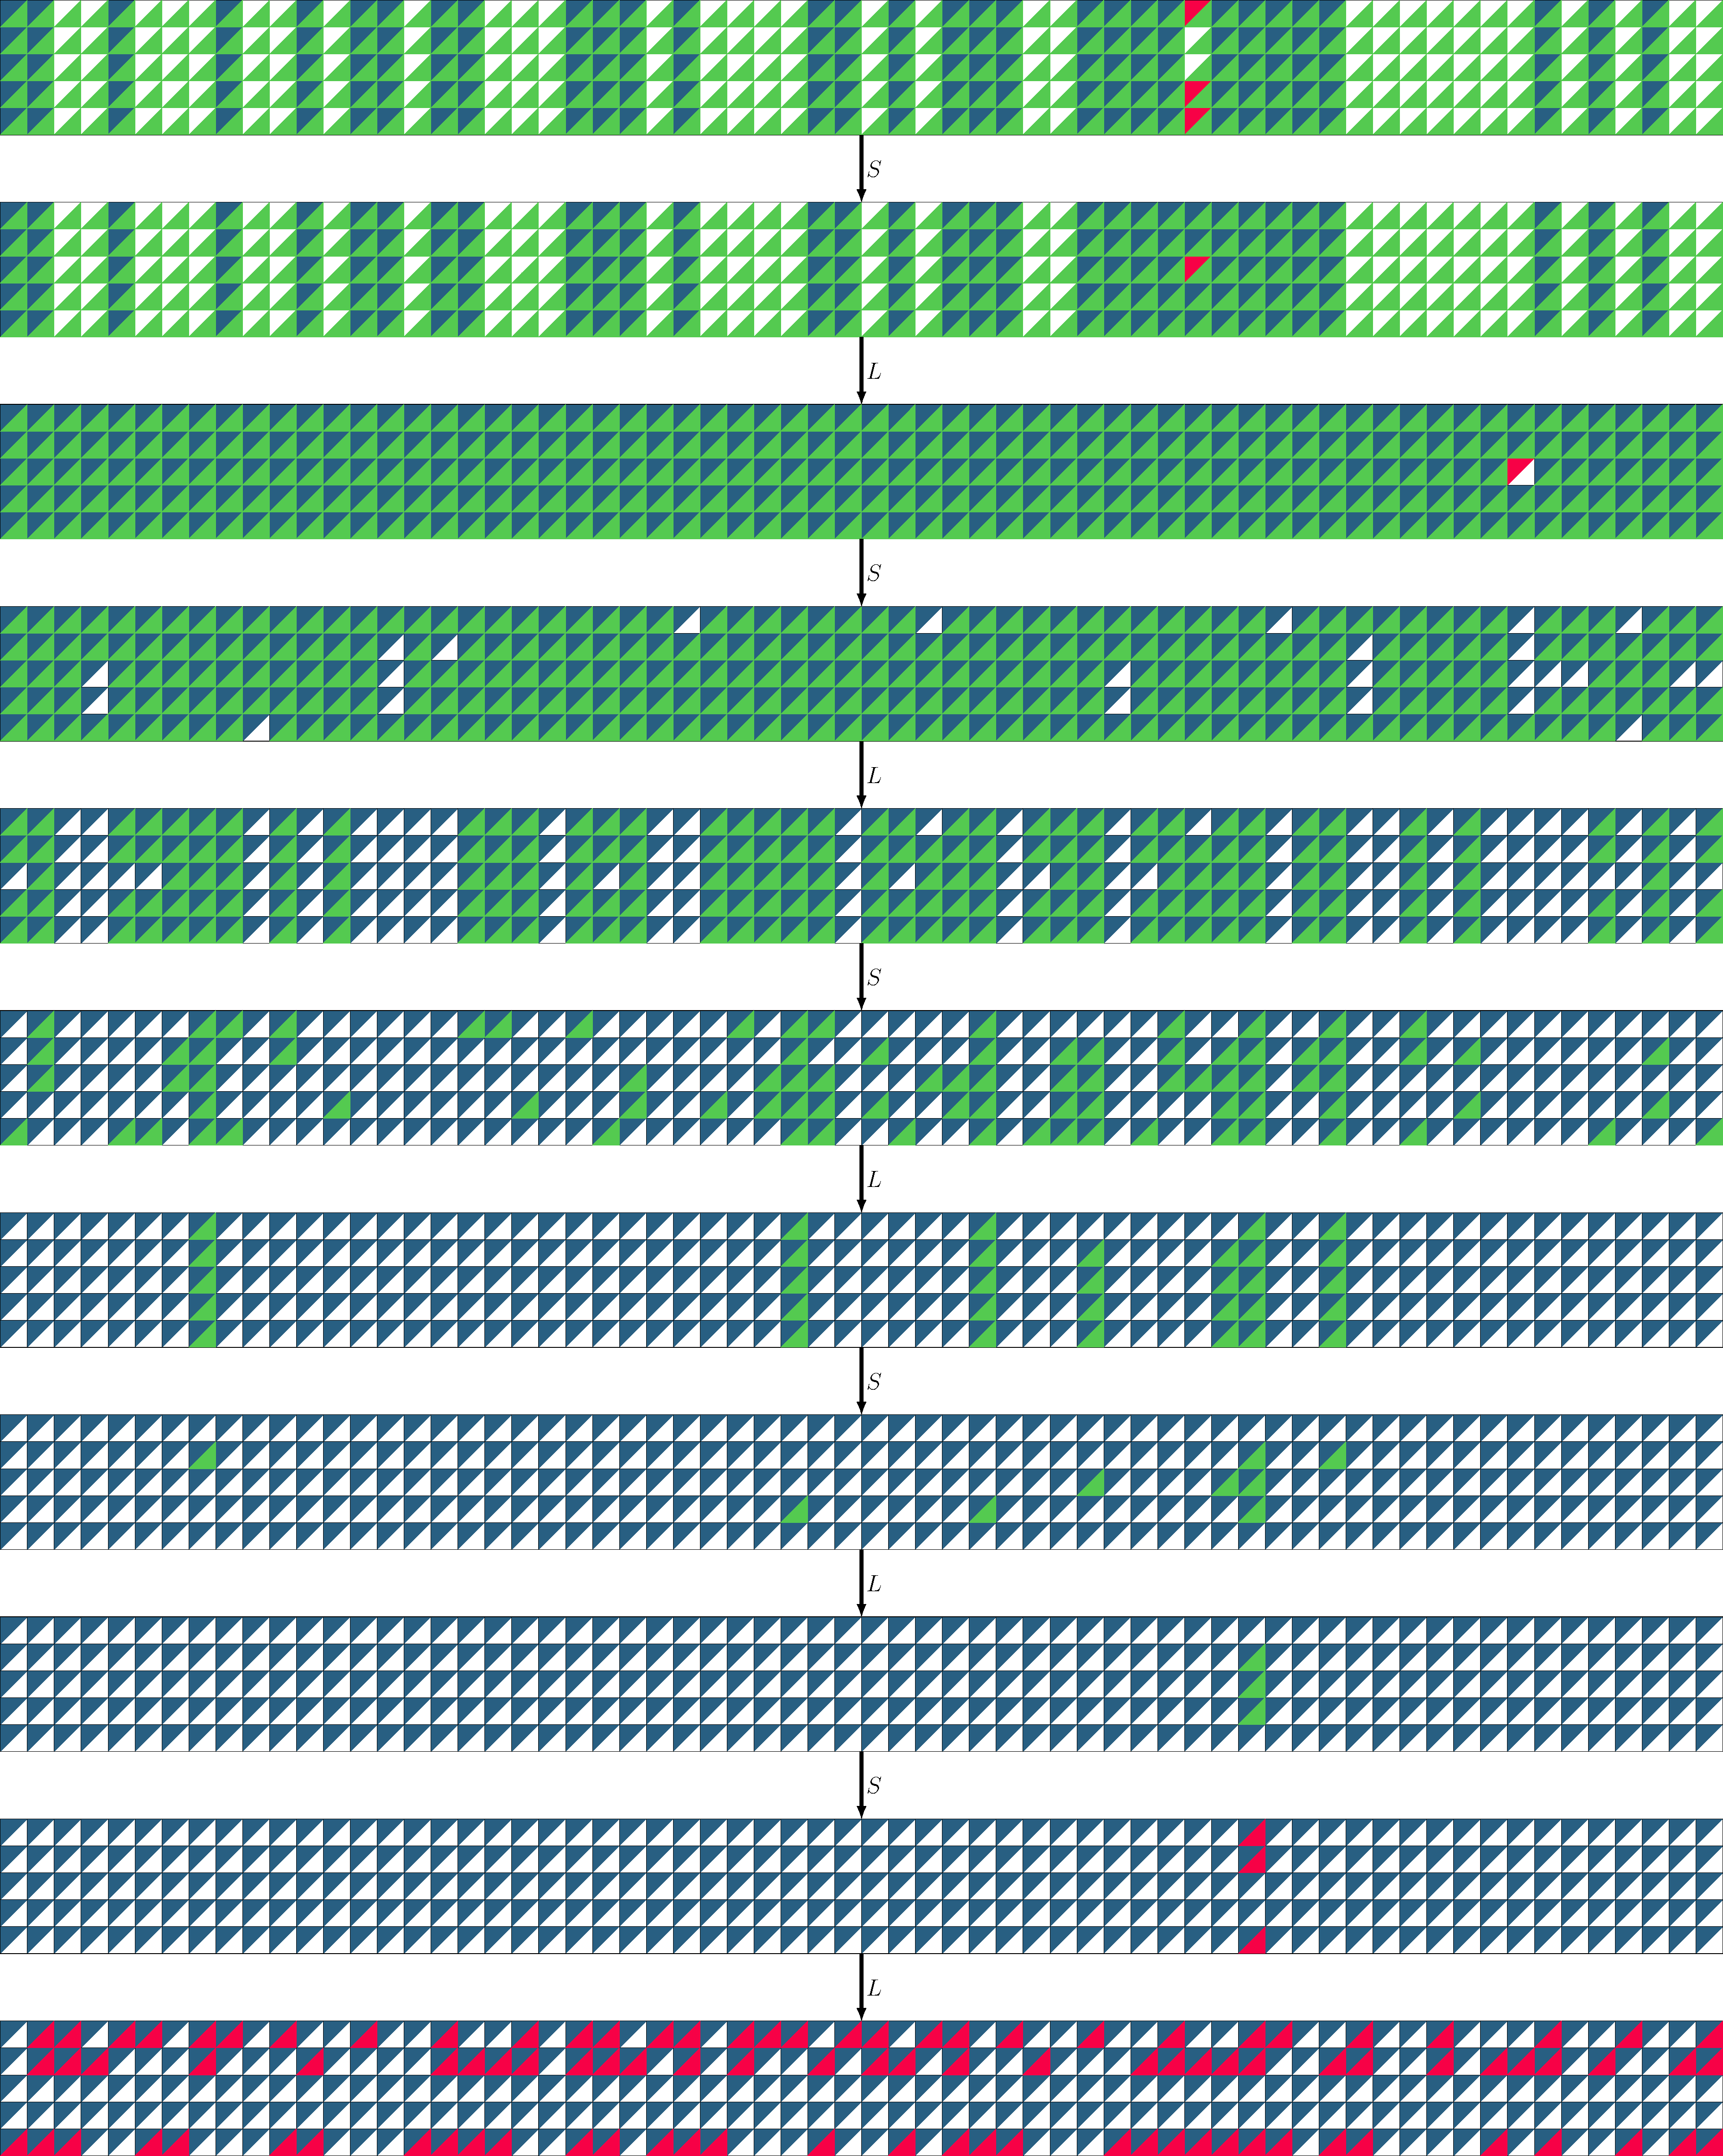
\includegraphics[width=0.62\textwidth]{./figures/ascon_zc_5r.pdf}
\caption*{\scriptsize $2^{155}$ ZC Distinguishers (upper/lower nonzero: \scalebox{0.5}{\legendwrap{\TFill[nonzeroany]{0,0}}}/\scalebox{0.5}{\legendwrap{\BFill[nonzeroany]{0,0}}})}
\end{figure}
\column[c]{0.50\textwidth}
\centering
\begin{figure}
\centering
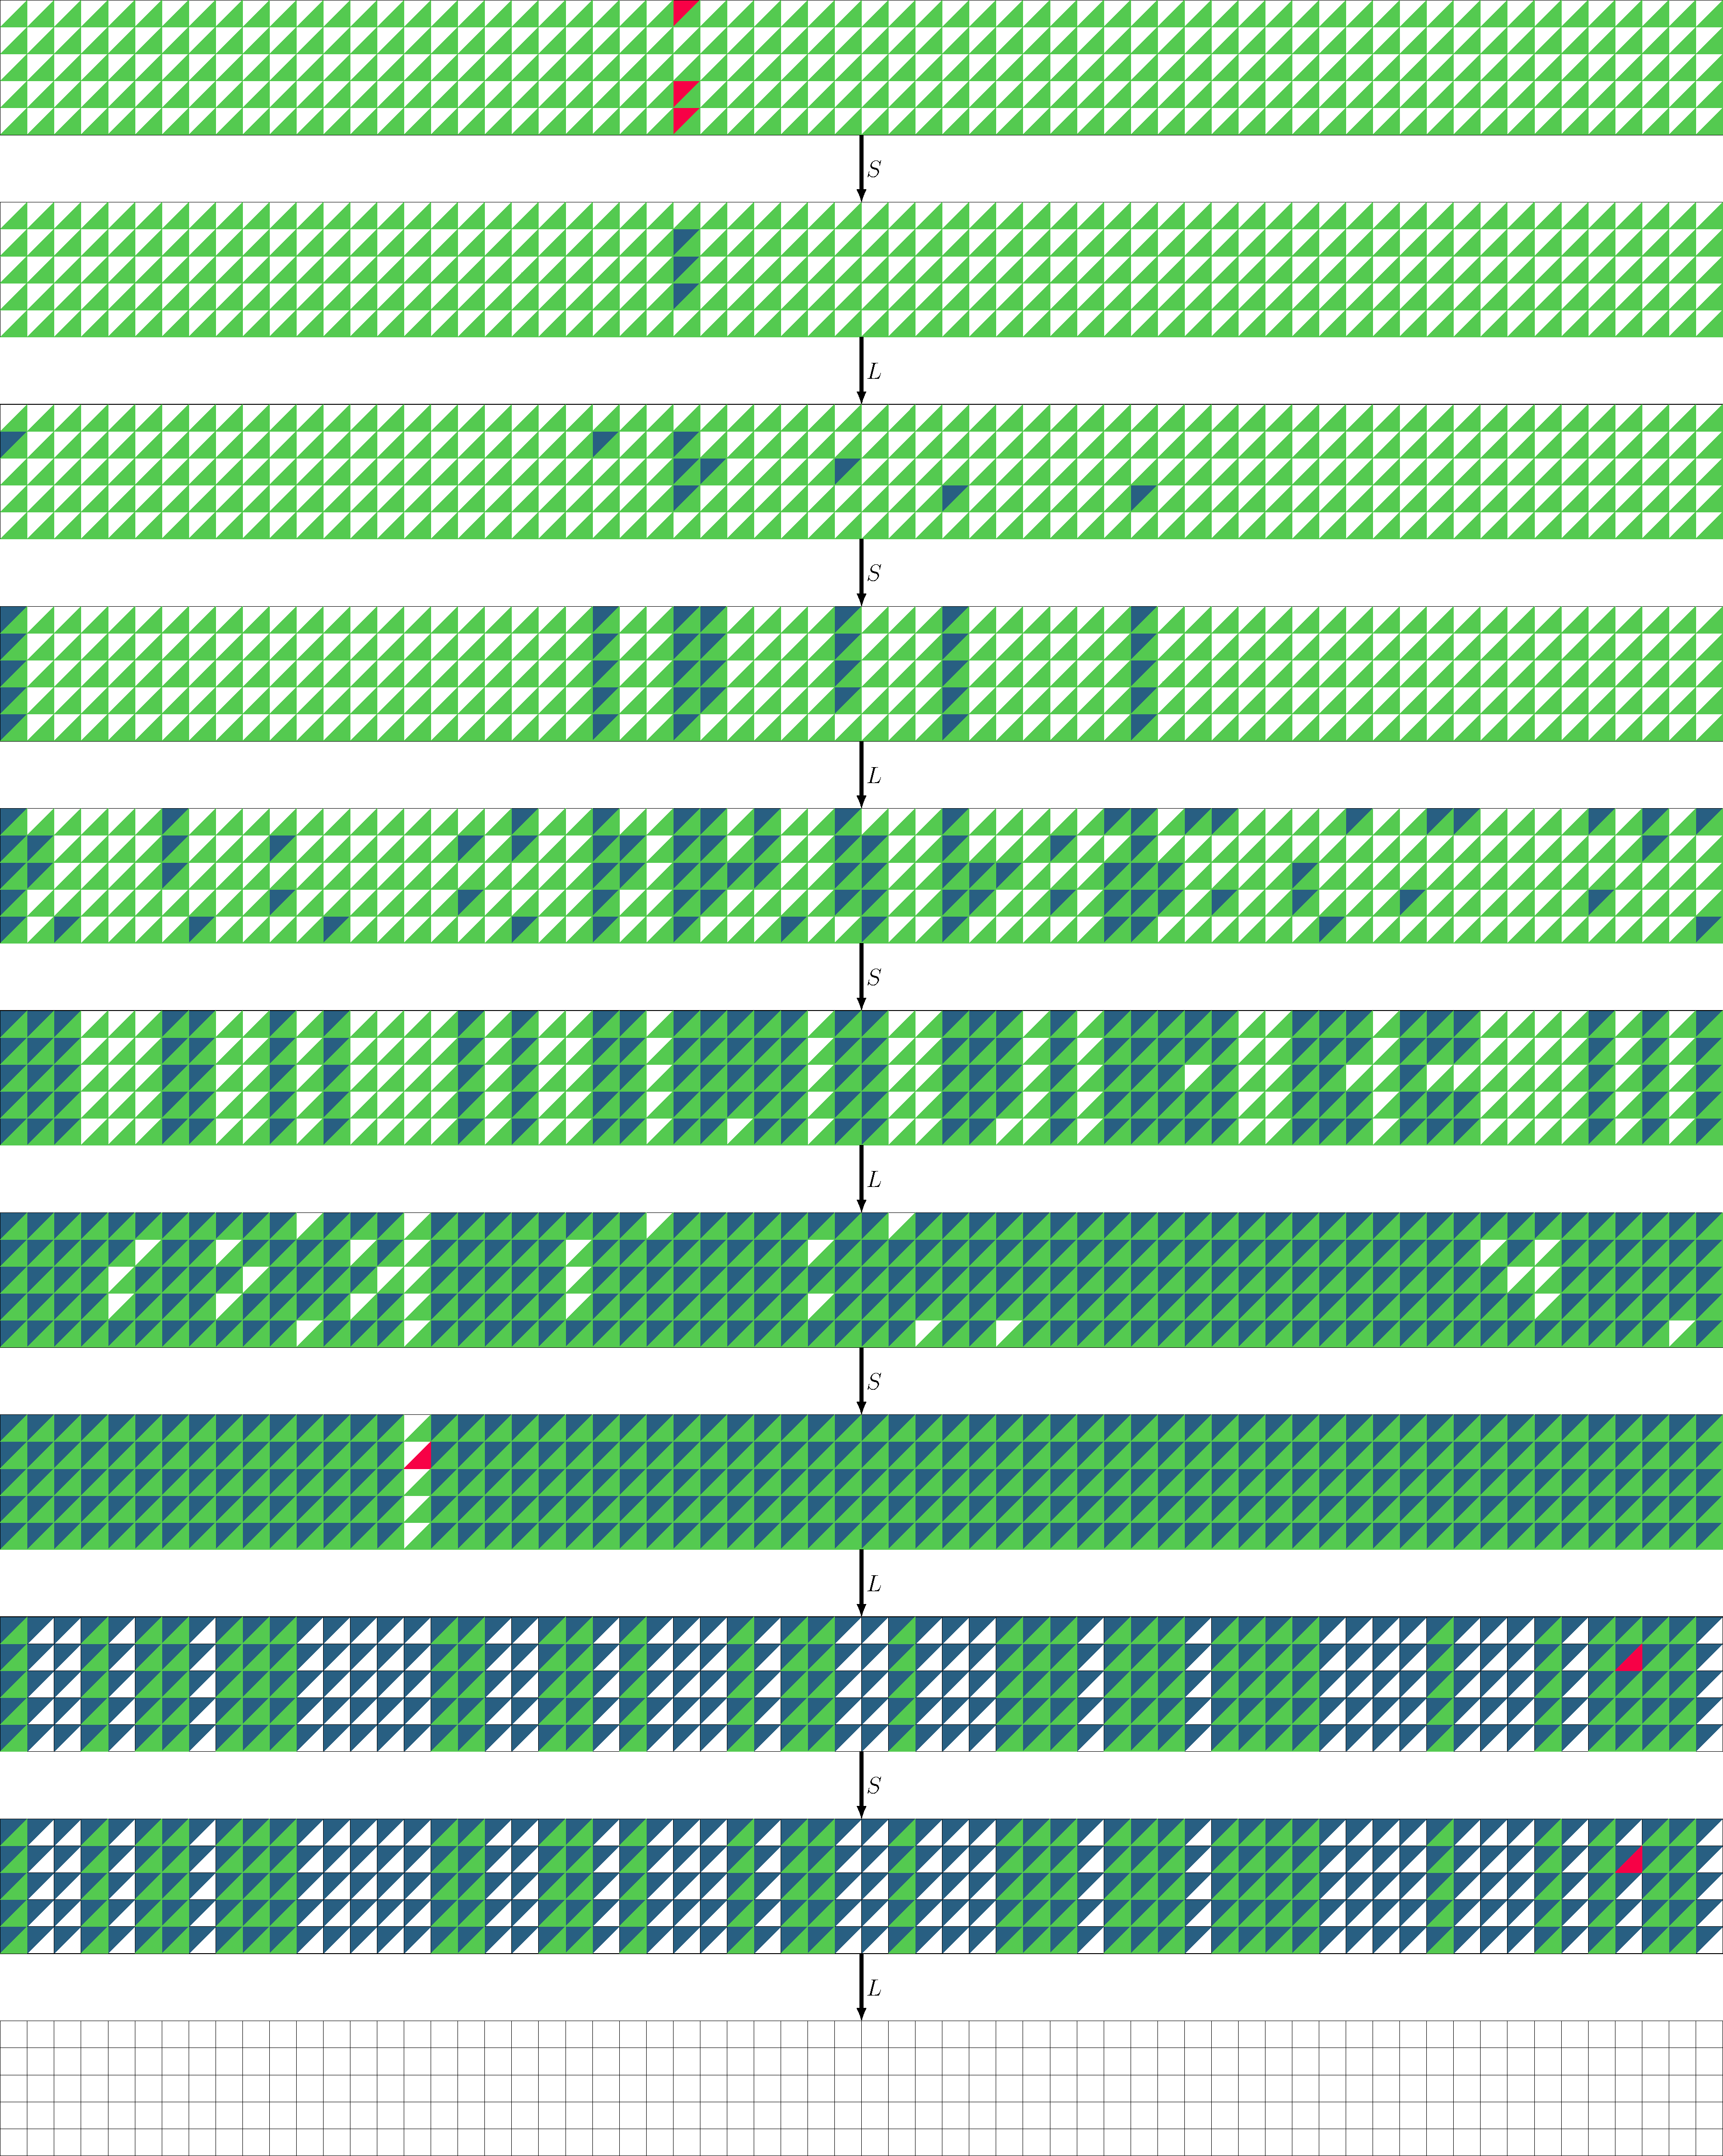
\includegraphics[width=0.62\textwidth]{./figures/ascon_id_5r_sll_v0.pdf}
\caption*{\scriptsize $2^{155}$ ID Distinguishers (upper/lower unknown: \scalebox{0.5}{\legendwrap{\TFill[upperunknown]{0,0}}}/\scalebox{0.5}{\legendwrap{\BFill[lowerunknown]{0,0}}})}
\end{figure}
\end{columns}
\end{frame}

%%%%%%%%%%%%%%%%%%%%%%%%%%%%%%%%%%%%%%%%%%%%%%%%%%%%%%%%%%%%%%%%%%%%%%%%
\begin{frame}{The Advantages of Our Method to Search for Distinguishers}
\begin{itemize}
  \small
  \item[\faCheckCircle] Based on satisfiability of the CP model
  \item[\faCheckCircle] Any feasible solutions of our CP model is a distinguisher
  \item[\faCheckCircle] We do not fix the input/output of distinguisher
  \item[\faDiamond] Extendable to a unified model for key-recovery
  \begin{itemize}
    \item[\faCheckCircle] Enables us to find a distinguisher optimized for key-recovery
    \item[\faCheckCircle] Enables us to consider key-recovery techniques:
    \begin{itemize}
      \item[\faCheckCircle] MitM
      \item[\faCheckCircle] Key bridging
      \item[\faCheckCircleO] \emph{Partial-sum technique}
    \end{itemize}
  \end{itemize}
\end{itemize}
\end{frame}

%%%%%%%%%%%%%%%%%%%%%%%%%%%%%%%%%%%%%%%%%%%%%%%%%%%%%%%%%%%%%%%%%%%%%%%%
%%%%%%%%%%%%%%%%%%%%%%%%%%%%%%%%%%%%%%%%%%%%%%%%%%%%%%%%%%%%%%%%%%%%%%%%
\section{Our Unified CP Model for Key-Recovery}
\sectionheader[\huge\color{tug}\faKey]{Our Unified CP Model for Partial-Sum Key-Recovery}

%%%%%%%%%%%%%%%%%%%%%%%%%%%%%%%%%%%%%%%%%%%%%%%%%%%%%%%%%%%%%%%%%%%%%%%%
%%%%%%%%%%%%%%%%%%%%%%%%%%%%%%%%%%%%%%%%%%%%%%%%%%%%%%%%%%%%%%%%%%%%%%%%%%%%%%%
\begin{frame}{Naive Approach v.s. Partial-Sum Technique}
\vspace{-0.5cm}
\begin{columns}
\column[c]{.62\textwidth}
\begin{itemize}
\small
\item[\faCab] Naive approach:
\begin{itemize}
  \small
	\item[\faCheckCircleO] $\bm{x} = F(\bm{k}, \bm{c})$ 
	\item[\faCheckCircleO] $T = N \cdot 2^{|\bm{k}|}$
\end{itemize}
\item<2->[\faFighterJet] Partial-sum technique:
\begin{itemize}
  \small
	\item<2->[\faCheckCircle] $\!\bm{x}_{1}\!=\!f_{1}(\bm{k}_{1}, \bm{x}_{0}),\!\bm{x}_{2}\!=\!f_{2}(\bm{k}_{2},\!\bm{x}_{1})\!,\cdots\!,\!\bm{x}\!=\!f_{n}(\bm{k}_{n}, \bm{x}_{n-1})$	
	\item<2->[\faCheckCircle] $\!\bm{x}_{0} = \bm{c}, N_{0} = N, N_{i} < N$
	\item<2->[\faCheckCircle] $\!T = \sum_{i = 1}^{n} \frac{N_{i - 1}}{n}\cdot 2^{|\bm{k}_{1}| + \cdots + |\bm{k}_{i}|} < \sum_{i = 1}^{n} \frac{N}{n} \cdot 2^{|\bm{k}|}$
	\item<2->[\faCheckCircle] $T < N\cdot 2^{|\bm{k}|}$ 
\end{itemize}
\end{itemize}
\column[c]{0.38\textwidth}
\centering
\null
\vspace{0.5cm}
\begin{figure}
\centering
\begin{subfigure}{0.49\textwidth}
\centering
\begin{tikzpicture}[xscale=1,yscale=1, charfont/.style={font=\scriptsize}]
\pgfmathsetmacro{\dx}{0.7}
\pgfmathsetmacro{\hdx}{\dx/2}
\pgfmathsetmacro{\dy}{0.5}
\pgfmathsetmacro{\hdy}{\dy/2}
\pgfmathsetmacro{\lxe}{2.7}
\pgfmathsetmacro{\lye}{1.2}
\coordinate (tleu) at (0,0);
\draw[rounded corners=0.1cm] (tleu) rectangle ++(\lxe,-\lye) coordinate (breu);
\coordinate (meu) at ($(tleu)!0.5!(breu)$);
\node at ($(tleu)!0.5!(breu) + (0, 0.7*\dy)$) {\textcolor{tugred}{$F$}};
\fill[fill=tuggray, opacity=0.6] ($(tleu) + (0, -\lye/2 + 0.05)$) -- ($(tleu) + (0, -\lye/2 - 0.05)$) -- ($(breu) + (0, 0.1)$) -- ($(breu) + (0, \lye - 0.1)$) -- cycle;
\node (x) at ($(tleu|-meu)+(-\dx,0)$) {$\bm{x}$};
\node (c) at ($(breu|-meu)+(\dx,0)$) {$\bm{c}$};
\node (k) at ($(tleu-|meu)+(0,1.5*\dy)$) {$\bm{k}$};
\draw[->] (c) -- ++(-\dx, 0);
\draw[<-] (x) -- ++(\dx, 0);
\draw[->] (k) -- ++(0, -1.5*\dy);
\end{tikzpicture}
\end{subfigure}
\vskip 0.5cm

\visible<2>{
\begin{subfigure}{0.49\textwidth}
\centering
\begin{tikzpicture}[xscale=1,yscale=1, charfont/.style={font=\scriptsize}]
\pgfmathsetmacro{\dx}{0.7}
\pgfmathsetmacro{\hdx}{\dx/2}
\pgfmathsetmacro{\dy}{0.5}
\pgfmathsetmacro{\hdy}{\dy/2}
\pgfmathsetmacro{\lxe}{2.7}
\pgfmathsetmacro{\lye}{1.2}
\coordinate (tleu) at (0,0);
\draw[rounded corners=0.1cm] (tleu) rectangle ++(\lxe,-\lye) coordinate (breu);
\coordinate (meu) at ($(tleu)!0.5!(breu)$);
\node at ($(tleu)!0.5!(breu) + (0, 0.7*\dy)$) {\textcolor{tugred}{$F$}};
\fill[fill=tuggray, opacity=0.6] ($(tleu) + (0, -\lye/2 + 0.05)$) -- ($(tleu) + (0, -\lye/2 - 0.05)$) -- ($(breu) + (0, 0.1)$) -- ($(breu) + (0, \lye - 0.1)$) -- cycle;
\node (x) at ($(tleu|-meu)+(-\dx,0)$) {$\bm{x}$};
\node (c) at ($(breu|-meu)+(\dx,0)$) {$\bm{c}$};
\node (k) at ($(tleu-|meu)+(0,1.5*\dy)$) {};
\draw[->] (c) -- ++(-\dx, 0);
\draw[<-] (x) -- ++(\dx, 0);

\node[] (x1) at ($(breu) + (-\lxe/8,+\lye/2)$) {$\bm{x}_{1}$};
\node[] (x2) at ($(breu) + (-\lxe*3/8,+\lye/2)$) {$\bm{x}_{2}$};
\node[rotate=00] (td) at ($(breu) + (-\lxe*5/9,+\lye/2)$) {$\cdots$};
\node[] (xn) at ($(tleu) + (\lxe/6,-\lye/2)$) {$\bm{x}_{n - 1}$};
\node (k1) at (x1|-k) {$\bm{k}_{1}$};
\node (k2) at (x2|-k) {$\bm{k}_{2}$};
\node (ttd) at (td|-k) {$\cdots$};
\node (kn) at (xn|-k) {$\bm{k}_{n}$};
\draw[->] (k1) -- ++(0, -1.5*\dy);
\draw[->] (k2) -- ++(0, -1.5*\dy);
\draw[->] (kn) -- ++(0, -1.5*\dy);
\end{tikzpicture}
\end{subfigure}}
\end{figure}
\end{columns}
\end{frame}

%%%%%%%%%%%%%%%%%%%%%%%%%%%%%%%%%%%%%%%%%%%%%%%%%%%%%%%%%%%%%%%%%%%%%%%%
\begin{frame}{Example: Partial-Sum Integral Key Recovery for AES \cite{fseFergusonKLSSWW00}}
\sparen
\begin{figure}
\centering
\begin{tikzpicture}[>=latex,xscale=1.35,remember picture,
                    stateopts/.style={scale=.25},
                    sbox/.style={draw,rounded corners=3pt, scale=.6}]
  \pgfmathsetmacro{\statesep}{1.5}

  \draw[every node/.style={state}] %, rounded corners=2pt]
  (-1, 0) node (SI) {\State{\Cell{ss00}{\tiny \texttt{0}} \Cell{ss10}{\tiny \texttt{1}} \Cell{ss20}{\tiny \texttt{2}} \Cell{ss30}{\tiny \texttt{3}}
  \Cell{ss01}{\tiny \texttt{4}} \Cell{ss11}{\tiny \texttt{5}} \Cell{ss21}{\tiny \texttt{6}} \Cell{ss31}{\tiny \texttt{7}}
  \Cell{ss02}{\tiny \texttt{8}} \Cell{ss12}{\tiny \texttt{9}} \Cell{ss22}{\tiny \texttt{10}}\Cell{ss32}{\tiny \texttt{11}}
  \Cell{ss03}{\tiny \texttt{12}} \Cell{ss13}{\tiny \texttt{13}} \Cell{ss23}{\tiny \texttt{14}} \Cell{ss33}{\tiny \texttt{15}}
  \iAct{ss00}\iAct{ss11}\iAct{ss22}\iAct{ss33}}}
  ++(0.9,-.9) node (SKI) {\State{\Cell{ss00}{\tiny \texttt{0}} \Cell{ss10}{\tiny \texttt{1}} \Cell{ss20}{\tiny \texttt{2}} \Cell{ss30}{\tiny \texttt{3}}
  \Cell{ss01}{\tiny \texttt{4}} \Cell{ss11}{\tiny \texttt{5}} \Cell{ss21}{\tiny \texttt{6}} \Cell{ss31}{\tiny \texttt{7}}
  \Cell{ss02}{\tiny \texttt{8}} \Cell{ss12}{\tiny \texttt{9}} \Cell{ss22}{\tiny \texttt{10}}\Cell{ss32}{\tiny \texttt{11}}
  \Cell{ss03}{\tiny \texttt{12}} \Cell{ss13}{\tiny \texttt{13}} \Cell{ss23}{\tiny \texttt{14}} \Cell{ss33}{\tiny \texttt{15}}
  }} ++(.65,-.4) node {\footnotesize $K_{0}$};
  \draw (SI) ++(0.9,0) coordinate[xor] (xori);
  \draw[->] (SI.east) -- (xori);
  \draw[->] (SKI) -- (xori);  
  % States
  \draw[every node/.style={state}] %, rounded corners=2pt]        
  ++(\statesep,0) node (S4) {\State{\foreach \b in {0,...,15} {\iBal{s\b}}}}
  ++(\statesep,0) +(0,-.9) node (SK5) {\State{\iKey{s0}{4} }}
  ++(0.65*\statesep,0) node (S5) {\State{\iPartial{s0}{4} }}
  ++(\statesep,0) +(0,-.9) node (SK6) {\State{\foreach \b/\s in {0/1,7/3,10/2,13/1} {\iKey{s\b}{\s}} }}
  ++(\statesep*.75,0) node (S6) {\State{\foreach \b/\s in {0/1,7/3,10/2,13/1} {\iStep{s\b}{\s}} }};
  \draw[->] (xori) -- node[above]{\small 4 rounds} (S4.west);
  \draw (S4) ++(0,-.8) node {\footnotesize $C_4$};
  \draw (S5) ++(0,-.8) node {\footnotesize $C_5$};
  \draw (S6) ++(0,-.8) node {\footnotesize $C_6$};
  \draw (SK5) ++(.65,-.4) node {\footnotesize $\bar{K}_5$};
  \draw (SK6) ++(.65,-.4) node {\footnotesize $K_6$};

  % Operations
  % \draw (\statesep/2,0) node[font=\fontsize{5}{5}\selectfont,align=center] {SB\\SR\\MC\\AK};
  \draw ($(S4.east) + (0.2, 0)$) node[font=\fontsize{5}{5}\selectfont,align=center] (Op5) {SB\\SR};
  \draw ($(S5.east) + (0.2, 0)$) node[font=\fontsize{5}{5}\selectfont,align=center] (Op6) {MC\\SB\\SR};


  \foreach \r in {5,6} {
    \draw (SK\r) ++(0,.9) coordinate[xor] (xor\r);
    \draw[->] (xor\r.east) -- (S\r.west);
    \draw[->] (Op\r.east) -- (xor\r.west);
    \draw[->] (SK\r.north) -- (xor\r.south);
  }
\end{tikzpicture}
\end{figure}
\sparen
\sparen
\begin{center}
\bgroup
\begin{align*}
  C_{4}[0] &=  \mathcal{S}^{-1}\left(\bar{K}_{5}[0] \oplus \texttt{0E} \cdot \mathcal{S}^{-1}\left(C_{6}[0] \oplus K_{6}[0]\right) \oplus \texttt{09} \cdot \mathcal{S}^{-1}\left(C_{6}[7] \oplus K_{6}[7]\right) \right. \nonumber\\
              & \left. ~\oplus \texttt{0D} \cdot \mathcal{S}^{-1}\left(C_{6}[10] \oplus K_{6}[10]\right) \oplus \texttt{0B} \cdot \mathcal{S}^{-1}\left(C_{6}[13] \oplus K_{6}[13]\right)\right)
\end{align*}
\egroup
\end{center}
\begin{itemize}
\item<1-> Time complexity of naive key recovery: $6\times 2^{32} \times 2^{40} \approx 2^{74.58}$
\end{itemize}
\end{frame}

%%%%%%%%%%%%%%%%%%%%%%%%%%%%%%%%%%%%%%%%%%%%%%%%%%%%%%%%%%%%%%%%%%%%%%%%
\begin{frame}{Partial-sum Technique for Integral Key Recovery \cite{fseFergusonKLSSWW00}}
\begin{columns}
\sparen
\column[c]{0.50\textwidth}
\centering
\resizebox{\textwidth}{!}{%
\begin{tikzpicture}[>=latex,xscale=1.35,remember picture,
                    stateopts/.style={scale=.25},
                    sbox/.style={draw,rounded corners=3pt, scale=.6}]
  \pgfmathsetmacro{\statesep}{1.5}

  \draw[every node/.style={state}] %, rounded corners=2pt]
  (-1, 0) node (SI) {\State{\Cell{ss00}{\tiny \texttt{0}} \Cell{ss10}{\tiny \texttt{1}} \Cell{ss20}{\tiny \texttt{2}} \Cell{ss30}{\tiny \texttt{3}}
  \Cell{ss01}{\tiny \texttt{4}} \Cell{ss11}{\tiny \texttt{5}} \Cell{ss21}{\tiny \texttt{6}} \Cell{ss31}{\tiny \texttt{7}}
  \Cell{ss02}{\tiny \texttt{8}} \Cell{ss12}{\tiny \texttt{9}} \Cell{ss22}{\tiny \texttt{10}}\Cell{ss32}{\tiny \texttt{11}}
  \Cell{ss03}{\tiny \texttt{12}} \Cell{ss13}{\tiny \texttt{13}} \Cell{ss23}{\tiny \texttt{14}} \Cell{ss33}{\tiny \texttt{15}}
  \iAct{ss00}\iAct{ss11}\iAct{ss22}\iAct{ss33}}}
  ++(0.9,-.9) node (SKI) {\State{\Cell{ss00}{\tiny \texttt{0}} \Cell{ss10}{\tiny \texttt{1}} \Cell{ss20}{\tiny \texttt{2}} \Cell{ss30}{\tiny \texttt{3}}
  \Cell{ss01}{\tiny \texttt{4}} \Cell{ss11}{\tiny \texttt{5}} \Cell{ss21}{\tiny \texttt{6}} \Cell{ss31}{\tiny \texttt{7}}
  \Cell{ss02}{\tiny \texttt{8}} \Cell{ss12}{\tiny \texttt{9}} \Cell{ss22}{\tiny \texttt{10}}\Cell{ss32}{\tiny \texttt{11}}
  \Cell{ss03}{\tiny \texttt{12}} \Cell{ss13}{\tiny \texttt{13}} \Cell{ss23}{\tiny \texttt{14}} \Cell{ss33}{\tiny \texttt{15}}
  }} ++(.65,-.4) node {\footnotesize $K_{0}$};
  \draw (SI) ++(0.9,0) coordinate[xor] (xori);
  \draw[->] (SI.east) -- (xori);
  \draw[->] (SKI) -- (xori);  
  % States
  \draw[every node/.style={state}] %, rounded corners=2pt]        
  ++(\statesep,0) node (S4) {\State{\foreach \b in {0,...,15} {\iBal{s\b}}}}
  ++(\statesep,0) +(0,-.9) node (SK5) {\State{\iKey{s0}{4} }}
  ++(0.65*\statesep,0) node (S5) {\State{\iPartial{s0}{4} }}
  ++(\statesep,0) +(0,-.9) node (SK6) {\State{\foreach \b/\s in {0/1,7/3,10/2,13/1} {\iKey{s\b}{\s}} }}
  ++(\statesep*.75,0) node (S6) {\State{\foreach \b/\s in {0/1,7/3,10/2,13/1} {\iStep{s\b}{\s}} }};
  \draw[->] (xori) -- node[above]{\small 4 rounds} (S4.west);
  \draw (S4) ++(0,-.8) node {\footnotesize $C_4$};
  \draw (S5) ++(0,-.8) node {\footnotesize $C_5$};
  \draw (S6) ++(0,-.8) node {\footnotesize $C_6$};
  \draw (SK5) ++(.65,-.4) node {\footnotesize $\bar{K}_5$};
  \draw (SK6) ++(.65,-.4) node {\footnotesize $K_6$};

  % Operations
  % \draw (\statesep/2,0) node[font=\fontsize{5}{5}\selectfont,align=center] {SB\\SR\\MC\\AK};
  \draw ($(S4.east) + (0.2, 0)$) node[font=\fontsize{5}{5}\selectfont,align=center] (Op5) {SB\\SR};
  \draw ($(S5.east) + (0.2, 0)$) node[font=\fontsize{5}{5}\selectfont,align=center] (Op6) {MC\\SB\\SR};


  \foreach \r in {5,6} {
    \draw (SK\r) ++(0,.9) coordinate[xor] (xor\r);
    \draw[->] (xor\r.east) -- (S\r.west);
    \draw[->] (Op\r.east) -- (xor\r.west);
    \draw[->] (SK\r.north) -- (xor\r.south);
  }
\end{tikzpicture}}
\sparen
\sparen
\begin{itemize}
  \scriptsize
  \item Guess $K_{6}[0, 7]$ and derive $\mathcal{S}_{0}\left(C_{6}[0]\oplus K_{6}[0]\right) \oplus \mathcal{S}_{1}\left(C_{6}[7] \oplus K_{6}[7]\right)$
  \sparen
  \item Guess $K_{6}[10]$ and derive $\mathcal{S}_{2}\left(C_{6}[10] \oplus K_{6}[10]\right)$
  \sparen
  \item Guess $K_{6}[13]$ and derive $\mathcal{S}_{3}\left(C_{6}[13] \oplus K_{6}[13]\right)$
  \sparen
  \item Guess $\bar{K}_{5}[0]$ and derive $C_{4}[0]$
  \sparen
  \item Time complexity: $6\times 4\times 2^{48} \approx 2^{52}$ S-box lookups 
\end{itemize}
\column[c]{0.50\textwidth}
\centering
%\begin{tikzpicture}[>=latex,xscale=1.25,yscale=\PScale,remember picture]
\resizebox{\textwidth}{!}{%
\begin{tikzpicture}[xscale=1.25,yscale=\PScale,remember picture,
                    sbox/.style={draw,rounded corners=3pt, scale=.6}]
  \pgfmathsetmacro{\statesep}{1.5}

  \draw (0, -3) node[inner sep=0pt] (S51) {\PartialSumStepInit}
  ++(0, -2.67) node[inner sep=0pt] (S52) {\PartialSumStepTwo}
  ++(0, -2.42) node[inner sep=0pt] (S53) {\PartialSumStepThree}
  ++(0, -1.83) node[inner sep=0pt] (S54) {\PartialSumStepFinal};
  \draw (sbox.south) coordinate (branch1);

  \draw (S51.north) ++(0,.3) node[inner sep=0pt] (X) {\footnotesize $C^0$};
  
  \draw (S51.north west) ++(-.3,0) node[inner sep=0pt, anchor=north east, align=right] (X) {\footnotesize Step 1: $\text{Key}= 2^{16}$ \\ \footnotesize $\text{Data} = 2^{32}$ \\ \footnotesize $\text{Time} = 2^{48}$};
  \draw (S52.north west) ++(-.3,0) node[inner sep=0pt, anchor=north east, align=right] (X) {\footnotesize Step 2: $\text{Key}= 2^{24}$ \\ \footnotesize $\text{Data} = 2^{24}$ \\ \footnotesize $\text{Time} = 2^{48}$};
  \draw (S53.north west) ++(-.3,0) node[inner sep=0pt, anchor=north east, align=right] (X) {\footnotesize Step 3: $\text{Key}= 2^{32}$ \\ \footnotesize $\text{Data} = 2^{16}$ \\ \footnotesize $\text{Time} = 2^{48}$};
  \draw (S54.north west) ++(-.3,0) node[inner sep=0pt, anchor=north east, align=right] (X) {\footnotesize Step 4: $\text{Key}= 2^{40}$ \\ \footnotesize $\text{Data} = 2^{8}$ \\ \footnotesize $\text{Time} = 2^{48}$};

  % \draw (3, -3) node[inner sep=0pt] (S51) {\PartialSumStepInit}
  % ++(0, -2.67) node[inner sep=0pt] (S52) {\PartialSumStepTwo}
  % ++(0, -2.42) node[inner sep=0pt] (S53) {\PartialSumStepThree}
  % ++(0, -1.83) node[inner sep=0pt] (S54) {\PartialSumStepFinal};
  % \draw (sbox.south) coordinate (branch2);

  % \draw (S51.north) ++(0,.3) node[inner sep=0pt] (X) {\footnotesize $C^1$};
  \draw (2,-6) node (dots) {$\dots$};

  \draw (4.5, -3) node[inner sep=0pt] (S51) {\PartialSumStepInit}
  ++(0, -2.67) node[inner sep=0pt] (S52) {\PartialSumStepTwo}
  ++(0, -2.42) node[inner sep=0pt] (S53) {\PartialSumStepThree}
  ++(0, -1.83) node[inner sep=0pt] (S54) {\PartialSumStepFinal};
  \draw (sbox.south) coordinate (branchn);

  \draw (S51.north) ++(0,.3) node[inner sep=0pt] (X) {\footnotesize $C^{2^{32}-1}$};

  \draw (branch1-|dots) ++(0,-.2) coordinate[xor] (xor5);
  \draw (xor5) ++(0,-.5) node[inner sep=0pt] (c5) {\SingleCell{\iBal{s}}};
  \draw (c5.west) ++(-.05,0) node[inner sep=0pt, anchor=east] {\footnotesize is};
  \draw (c5.east) ++(.05,0) node[inner sep=0pt, anchor=west] {\footnotesize ?};
  \draw[->, rounded corners=2pt] (xor5.south) -- (c5.north);

  \draw[->, rounded corners=2pt] (branch1) |- (xor5.west);
  \draw[->, rounded corners=2pt] (branchn) |- (xor5.east);

  \draw (xor5-|dots) ++(1,0) node[inner sep=5pt,fill=white] {$\dots$};

\end{tikzpicture}}
\end{columns}
\end{frame}

%%%%%%%%%%%%%%%%%%%%%%%%%%%%%%%%%%%%%%%%%%%%%%%%%%%%%%%%%%%%%%%%%%%%%%%%
\begin{frame}{Our CP Model for Partial-Sum Technique - I}
\vspace{-0.7cm}
\begin{center}
  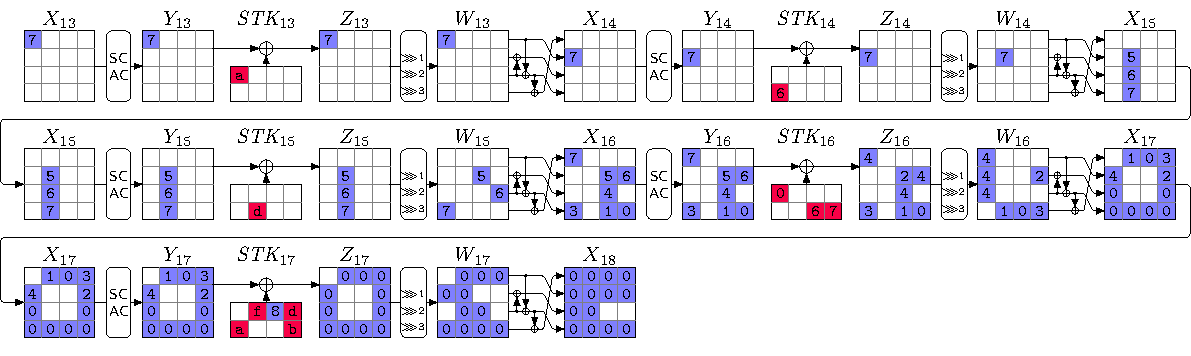
\includegraphics[width=0.8\textwidth]{./figures/zc_rt_skinny_tk1_18r_keyrec1.pdf}
\end{center}
\vspace{-0.9cm}
\begin{center}
  \scalebox{0.55}{
  \begin{tabular}[t]{@{}clc@{$\times$}c@{$=$}ccl@{}}
  \toprule
  Step & Guessed & \KeysData & Mem & Time & Stored Texts \\ \midrule
  0 & -- & $2^{0}$ & $2^{40}$ & $2^{40}$ & $2^{40-5.2}$ & $\textit{Z}_{17}[1, 3, 4, 7]$; $\textit{X}_{17}[8, 11, 12, 13, 15]$; $\textit{X}_{16}[15]$ \\
  1 & $\textit{STK}_{17}[1]$ & $2^{4}$ & $2^{36}$ & $2^{40}$ & $2^{44-7.2}$ & $\textit{Z}_{17}[3, 4, 7]$; $\textit{X}_{17}[8, 11, 12, 15]$; $\textit{X}_{16}[14, 15]$ \\
  2 & $\textit{STK}_{17}[7]$ & $2^{8}$ & $2^{32}$ & $2^{40}$ & $2^{44-8.2}$ & $\textit{Z}_{17}[3, 4]$; $\textit{X}_{17}[8, 12, 15]$; $\textit{Z}_{16}[6]$; $\textit{X}_{16}[14, 15]$ \\
  3 & $\textit{STK}_{17}[3]$ & $2^{12}$ & $2^{28}$ & $2^{40}$ & $2^{44-7.2}$ & $\textit{Z}_{17}[4]$; $\textit{X}_{17}[8, 12]$; $\textit{Z}_{16}[6]$; $\textit{X}_{16}[12, 14, 15]$ \\
  4 & $\textit{STK}_{17}[4]$ & $2^{16}$ & $2^{28}$ & $2^{44}$ & $2^{44-7.2}$ & $\textit{Z}_{16}[0, 6, 7]$; $\textit{X}_{16}[10, 12, 14, 15]$ \\
  5 & $\textit{STK}_{16}[6]$ & $2^{20}$ & $2^{20}$ & $2^{40}$ & $2^{48-7.2}$ & $\textit{Z}_{16}[0, 7]$; $\textit{X}_{16}[12, 15]$; $\textit{X}_{15}[5]$ \\
  6 & $\textit{STK}_{16}[7]$ & $2^{24}$ & $2^{16}$ & $2^{40}$ & $2^{44-7.2}$ & $\textit{Z}_{16}[0]$; $\textit{X}_{16}[12]$; $\textit{X}_{15}[5, 9]$ \\
  7 & $\textit{STK}_{16}[0]$ & $2^{28}$ & $2^{4}$ & $2^{32}$ & $2^{44-6.2}$ & $\textit{X}_{13}[0]$ \\
  $\Sigma$ & \multicolumn{3}{c}{} & $2^{44}$ & $2^{41.32}$ &  \\
  \bottomrule
  \end{tabular}}
\end{center}
\end{frame}

%%%%%%%%%%%%%%%%%%%%%%%%%%%%%%%%%%%%%%%%%%%%%%%%%%%%%%%%%%%%%%%%%%%%%%%%
\begin{frame}{Our CP Model for Partial-Sum Technique - II}
\begin{itemize}
  \item Assume that in each step we guess at least one cell of the involved keys.
  \item We define the number of steps $s$ which is less than the number of involved key cells. 
  \item For each cell we define an integer variable with domain $\{0, \cdots, $s$\}$.
  \item We define some constraints to compute the step number of deriving each cell.
\end{itemize}
\begin{center}
\scalebox{.7}{% TODO
\begin{tikzpicture}[baseline=0pt]
  \SkinnyInit{}{}{}{}
  \SkinnyRoundTK[20] % round number should be 0-indexed
                  {
                  \Cell{ss00}{\ttfamily 7}\Cell{ss01}{\ttfamily 5}\Cell{ss02}{\ttfamily 1}\Cell{ss03}{\ttfamily 3}\Cell{ss10}{\ttfamily 8}\Cell{ss11}{\ttfamily 9}\Cell{ss12}{\ttfamily 3}\Cell{ss13}{\ttfamily 8}
                  \Cell{ss22}{\ttfamily 6}\Cell{ss23}{\ttfamily 4}\Cell{ss30}{\ttfamily 1}\Cell{ss31}{\ttfamily 1}\Cell{ss32}{\ttfamily 1}\Cell{ss33}{\ttfamily 1}}
                  {
                  \Cell{ss00}{\ttfamily 7}\Cell{ss01}{\ttfamily 5}\Cell{ss02}{\ttfamily 1}\Cell{ss03}{\ttfamily 3}\Cell{ss10}{\ttfamily 8}\Cell{ss11}{\ttfamily 9}\Cell{ss12}{\ttfamily 3}\Cell{ss13}{\ttfamily 8}}{}{} % tk[1,2,3]
                  {
                  \Cell{ss00}{\ttfamily 7}\Cell{ss01}{\ttfamily 5}\Cell{ss02}{\ttfamily 1}\Cell{ss03}{\ttfamily 3}\Cell{ss10}{\ttfamily 8}\Cell{ss11}{\ttfamily 9}\Cell{ss12}{\ttfamily 3}\Cell{ss13}{\ttfamily 8}
                  \Cell{ss22}{\ttfamily 6}\Cell{ss23}{\ttfamily 4}\Cell{ss30}{\ttfamily 1}\Cell{ss31}{\ttfamily 1}\Cell{ss32}{\ttfamily 1}\Cell{ss33}{\ttfamily 1}}
                  {
                  \Cell{ss00}{\ttfamily 6}\Cell{ss01}{\ttfamily 4}\Cell{ss02}{\ttfamily 0}\Cell{ss03}{\ttfamily 2}\Cell{ss10}{\ttfamily 4}\Cell{ss11}{\ttfamily 0}\Cell{ss12}{\ttfamily 2}\Cell{ss13}{\ttfamily 6}
                  \Cell{ss22}{\ttfamily 6}\Cell{ss23}{\ttfamily 4}\Cell{ss30}{\ttfamily 1}\Cell{ss31}{\ttfamily 1}\Cell{ss32}{\ttfamily 1}\Cell{ss33}{\ttfamily 1}}
                  {\Fill[tugblue]{ss10}\Fill[tugcyan]{ss33}
                  \Cell{ss00}{\ttfamily 6}\Cell{ss01}{\ttfamily 4}\Cell{ss02}{\ttfamily 0}\Cell{ss03}{\ttfamily 2}\Cell{ss10}{\ttfamily 6}\Cell{ss11}{\ttfamily 4}\Cell{ss12}{\ttfamily 0}\Cell{ss13}{\ttfamily 2}
                  \Cell{ss20}{\ttfamily 6}\Cell{ss21}{\ttfamily 4}\Cell{ss30}{\ttfamily 1}\Cell{ss31}{\ttfamily 1}\Cell{ss32}{\ttfamily 1}\Cell{ss33}{\ttfamily 1}}

    \SkinnyNewLine[21]
                  {\Fill[tugblue]{ss10}\Fill[tugblue]{ss20}\Fill[tugblue]{ss30}\Fill[tugcyan]{ss03}\Fill[tugcyan]{ss33}
                  \Cell{ss00}{\ttfamily 1}\Cell{ss01}{\ttfamily 1}\Cell{ss02}{\ttfamily 1}\Cell{ss03}{\ttfamily 1}\Cell{ss10}{\ttfamily 6}\Cell{ss11}{\ttfamily 4}\Cell{ss12}{\ttfamily 0}\Cell{ss13}{\ttfamily 2}
                  \Cell{ss20}{\ttfamily 0}\Cell{ss21}{\ttfamily 0}\Cell{ss22}{\ttfamily 0}\Cell{ss23}{\ttfamily 0}\Cell{ss30}{\ttfamily 0}\Cell{ss31}{\ttfamily 0}\Cell{ss32}{\ttfamily 0}\Cell{ss33}{\ttfamily 0}} % state (input)
                  

    \SkinnyRoundTK[21] % round number should be 0-indexed
                  {
                  \Cell{ss00}{\ttfamily 1}\Cell{ss01}{\ttfamily 1}\Cell{ss02}{\ttfamily 1}\Cell{ss03}{\ttfamily 1}\Cell{ss10}{\ttfamily 6}\Cell{ss11}{\ttfamily 4}\Cell{ss12}{\ttfamily 0}\Cell{ss13}{\ttfamily 2}
                  \Cell{ss20}{\ttfamily 0}\Cell{ss21}{\ttfamily 0}\Cell{ss22}{\ttfamily 0}\Cell{ss23}{\ttfamily 0}\Cell{ss30}{\ttfamily 0}\Cell{ss31}{\ttfamily 0}\Cell{ss32}{\ttfamily 0}\Cell{ss33}{\ttfamily 0}} % state (input)
                {\Fill[tuggreen]{ss00}\Fill[tuggreen]{ss01}\Fill[tuggreen]{ss02}\Fill[tuggreen]{ss03}\Fill[tuggreen]{ss10}\Fill[tuggreen]{ss11}\Fill[tuggreen]{ss13}
                  \Cell{ss00}{\ttfamily 1}\Cell{ss01}{\ttfamily 1}\Cell{ss02}{\ttfamily 1}\Cell{ss03}{\ttfamily 1}\Cell{ss10}{\ttfamily 6}\Cell{ss11}{\ttfamily 4}\Cell{ss13}{\ttfamily 2}}{}{} % tk[1,2,3]
                  {
                  \Cell{ss00}{\ttfamily 1}\Cell{ss01}{\ttfamily 1}\Cell{ss02}{\ttfamily 1}\Cell{ss03}{\ttfamily 1}\Cell{ss10}{\ttfamily 6}\Cell{ss11}{\ttfamily 4}\Cell{ss12}{\ttfamily 0}\Cell{ss13}{\ttfamily 2}
                  \Cell{ss20}{\ttfamily 0}\Cell{ss21}{\ttfamily 0}\Cell{ss22}{\ttfamily 0}\Cell{ss23}{\ttfamily 0}\Cell{ss30}{\ttfamily 0}\Cell{ss31}{\ttfamily 0}\Cell{ss32}{\ttfamily 0}\Cell{ss33}{\ttfamily 0}} % state (after subcells)
                  {\Fill[tuggreen]{ss00}\Fill[tuggreen]{ss01}\Fill[tuggreen]{ss02}\Fill[tuggreen]{ss03}\Fill[tuggreen]{ss10}\Fill[tuggreen]{ss11}\Fill[tuggreen]{ss13}
                  \Cell{ss33}{\ttfamily 0}\Cell{ss32}{\ttfamily 0}\Cell{ss31}{\ttfamily 0}\Cell{ss30}{\ttfamily 0}\Cell{ss23}{\ttfamily 0}\Cell{ss22}{\ttfamily 0}\Cell{ss21}{\ttfamily 0}\Cell{ss20}{\ttfamily 0}
                  \Cell{ss13}{\ttfamily 0}\Cell{ss12}{\ttfamily 0}\Cell{ss11}{\ttfamily 0}\Cell{ss10}{\ttfamily 0}\Cell{ss03}{\ttfamily 0}\Cell{ss02}{\ttfamily 0}\Cell{ss01}{\ttfamily 0}\Cell{ss00}{\ttfamily 0}} % state (after addtweakey)
                  {
                  \Cell{ss33}{\ttfamily 0}\Cell{ss32}{\ttfamily 0}\Cell{ss31}{\ttfamily 0}\Cell{ss30}{\ttfamily 0}\Cell{ss23}{\ttfamily 0}\Cell{ss22}{\ttfamily 0}\Cell{ss21}{\ttfamily 0}\Cell{ss20}{\ttfamily 0}
                  \Cell{ss13}{\ttfamily 0}\Cell{ss12}{\ttfamily 0}\Cell{ss11}{\ttfamily 0}\Cell{ss10}{\ttfamily 0}\Cell{ss03}{\ttfamily 0}\Cell{ss02}{\ttfamily 0}\Cell{ss01}{\ttfamily 0}\Cell{ss00}{\ttfamily 0}} % state (after shiftrows)

    \SkinnyFin[22]
                  {
                  \Cell{ss33}{\ttfamily 0}\Cell{ss32}{\ttfamily 0}\Cell{ss31}{\ttfamily 0}\Cell{ss30}{\ttfamily 0}\Cell{ss23}{\ttfamily 0}\Cell{ss22}{\ttfamily 0}\Cell{ss21}{\ttfamily 0}\Cell{ss20}{\ttfamily 0}
                  \Cell{ss13}{\ttfamily 0}\Cell{ss12}{\ttfamily 0}\Cell{ss11}{\ttfamily 0}\Cell{ss10}{\ttfamily 0}\Cell{ss03}{\ttfamily 0}\Cell{ss02}{\ttfamily 0}\Cell{ss01}{\ttfamily 0}\Cell{ss00}{\ttfamily 0}}
\end{tikzpicture}
}
\end{center}
\end{frame}

%%%%%%%%%%%%%%%%%%%%%%%%%%%%%%%%%%%%%%%%%%%%%%%%%%%%%%%%%%%%%%%%%%%%%%%%
\begin{frame}{Our Unified Model for Finding Integral Attack}
\begin{columns}
\column[c]{\textwidth}
\begin{itemize}
\item Our CP model for finding complete integral attack includes the following modules:
\begin{itemize}
\item Model the distinguisher part
\item Model the meet-in-the-middle technique
\item Model the involved cells in key recovery
\item Model the step assignment
\item Model the tweakey schedule (key-bridging)
\item Model the time/memory complexity evaluation
\end{itemize}
\item Objective function: minimize the total time complexity
\end{itemize}
% \column[c]{0.6\textwidth}
% \sparen
% \sparen
% \begin{center}
%   \centering
%   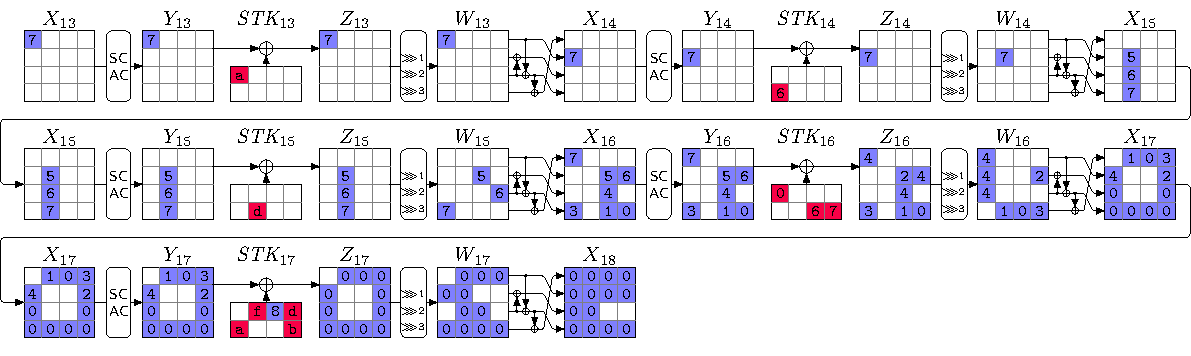
\includegraphics[width=\textwidth]{./figures/zc_rt_skinny_tk1_18r_keyrec1.pdf}
%   \resizebox{0.95\textwidth}{!}{
%   \begin{tabular}[t]{@{}clc@{$\times$}c@{$=$}ccl@{}}
%   \toprule
%   Step & Guessed & \KeysData & Mem & Time & Stored Texts \\ \midrule
%   0 & -- & $2^{0}$ & $2^{40}$ & $2^{40}$ & $2^{40-5.2}$ & $\textit{Z}_{17}[1, 3, 4, 7]$; $\textit{X}_{17}[8, 11, 12, 13, 15]$; $\textit{X}_{16}[15]$ \\
%   1 & $\textit{STK}_{17}[1]$ & $2^{4}$ & $2^{36}$ & $2^{40}$ & $2^{44-7.2}$ & $\textit{Z}_{17}[3, 4, 7]$; $\textit{X}_{17}[8, 11, 12, 15]$; $\textit{X}_{16}[14, 15]$ \\
%   2 & $\textit{STK}_{17}[7]$ & $2^{8}$ & $2^{32}$ & $2^{40}$ & $2^{44-8.2}$ & $\textit{Z}_{17}[3, 4]$; $\textit{X}_{17}[8, 12, 15]$; $\textit{Z}_{16}[6]$; $\textit{X}_{16}[14, 15]$ \\
%   3 & $\textit{STK}_{17}[3]$ & $2^{12}$ & $2^{28}$ & $2^{40}$ & $2^{44-7.2}$ & $\textit{Z}_{17}[4]$; $\textit{X}_{17}[8, 12]$; $\textit{Z}_{16}[6]$; $\textit{X}_{16}[12, 14, 15]$ \\
%   4 & $\textit{STK}_{17}[4]$ & $2^{16}$ & $2^{28}$ & $2^{44}$ & $2^{44-7.2}$ & $\textit{Z}_{16}[0, 6, 7]$; $\textit{X}_{16}[10, 12, 14, 15]$ \\
%   5 & $\textit{STK}_{16}[6]$ & $2^{20}$ & $2^{20}$ & $2^{40}$ & $2^{48-7.2}$ & $\textit{Z}_{16}[0, 7]$; $\textit{X}_{16}[12, 15]$; $\textit{X}_{15}[5]$ \\
%   6 & $\textit{STK}_{16}[7]$ & $2^{24}$ & $2^{16}$ & $2^{40}$ & $2^{44-7.2}$ & $\textit{Z}_{16}[0]$; $\textit{X}_{16}[12]$; $\textit{X}_{15}[5, 9]$ \\
%   7 & $\textit{STK}_{16}[0]$ & $2^{28}$ & $2^{4}$ & $2^{32}$ & $2^{44-6.2}$ & $\textit{X}_{13}[0]$ \\
%   $\Sigma$ & \multicolumn{3}{c}{} & $2^{44}$ & $2^{41.32}$ &  \\
%   \bottomrule
%   \end{tabular}}
% \end{center}
\end{columns}
\end{frame}

%%%%%%%%%%%%%%%%%%%%%%%%%%%%%%%%%%%%%%%%%%%%%%%%%%%%%%%%%%%%%%%%%%%%%%%%
\begin{frame}{Usage of Our Tool}
\begin{center}
\vspace{0.2cm}
{\large \texttt{python3 attack.py -RB \textcolor{tugred}{1} -RD \textcolor{tugred}{12} -RF \textcolor{tugred}{5}}}
\end{center}
\begin{figure}
\centering
\begin{tikzpicture}[yscale=1,xscale=1,baseline=0, decoration={
  markings,
  mark=at position 0.5 with {\arrow{>>}}}]
\pgfmathsetmacro{\hstep}{4}
\pgfmathsetmacro{\vstep}{1.4}
\pgfmathsetmacro{\halfvstep}{\vstep/2}
\pgfmathsetmacro{\quartervstep}{\vstep/4}
\pgfmathsetmacro{\halfhstep}{\hstep/2}
\pgfmathsetmacro{\quarterhstep}{\hstep/4}
\node[overlay] (c1) at (0, 0) {};
\node[overlay, right=\halfhstep of c1] (c2) {};
\node[overlay, right=\hstep of c2] (c3) {};
\node[overlay, right=\halfhstep of c3] (c4) {};	
\draw[rounded corners=2pt] ($(c1) + (0, -\halfvstep)$) rectangle ($(c4) + (0, \halfvstep)$);
\draw[] ($(c2) + (0, -\halfvstep)$) -- ($(c2) + (0, \halfvstep + 0.2)$);
\draw[] ($(c3) + (0, -\halfvstep)$) -- ($(c3) + (0, \halfvstep + 0.2)$);
\draw[<->, dashed] ($(c1) + (0, \halfvstep + 0.1)$) -- node[above] {$R\In$} ($(c2) + (0,\halfvstep + 0.1)$);
\draw[<->, dashed] ($(c2) + (0, \halfvstep + 0.1)$) -- node[above] {$R\Dist$} ($(c3) + (0,\halfvstep + 0.1)$);
\draw[<->, dashed] ($(c3) + (0, \halfvstep + 0.1)$) -- node[above] {$R\Out$} ($(c4) + (0,\halfvstep + 0.1)$);
\node[] (e0) at ($0.5*(c1) + 0.5*(c2)$) {$E\In$};
\node[] (e1) at ($0.5*(c2) + 0.5*(c3)$) {$E\Dist$};
\node[] (e2) at ($0.5*(c3) + 0.5*(c4)$) {$E\Out$};
\end{tikzpicture}
\end{figure}
\begin{itemize}
  \item[\faCheckCircle] We use MiniZinc \cite{cp_NethercoteSBBDT07} to create our CP models
  \item[\faCheckCircle] We use Gurobi \cite{gurobi} and OrTools \cite{ortools} as the CP solvers
  \item[\faLaptop] Our tool can find the results in a few seconds running on a regular laptop
\end{itemize}
\end{frame}

%%%%%%%%%%%%%%%%%%%%%%%%%%%%%%%%%%%%%%%%%%%%%%%%%%%%%%%%%%%%%%%%%%%%%%%%%%%%%%%
\begin{frame}{Example: 18-round Integral Attack on SKINNY-$n$-$n$}
\vspace{-0.75cm}
\begin{columns}
\column[c]{0.5\textwidth}
\begin{figure}
  \centering
  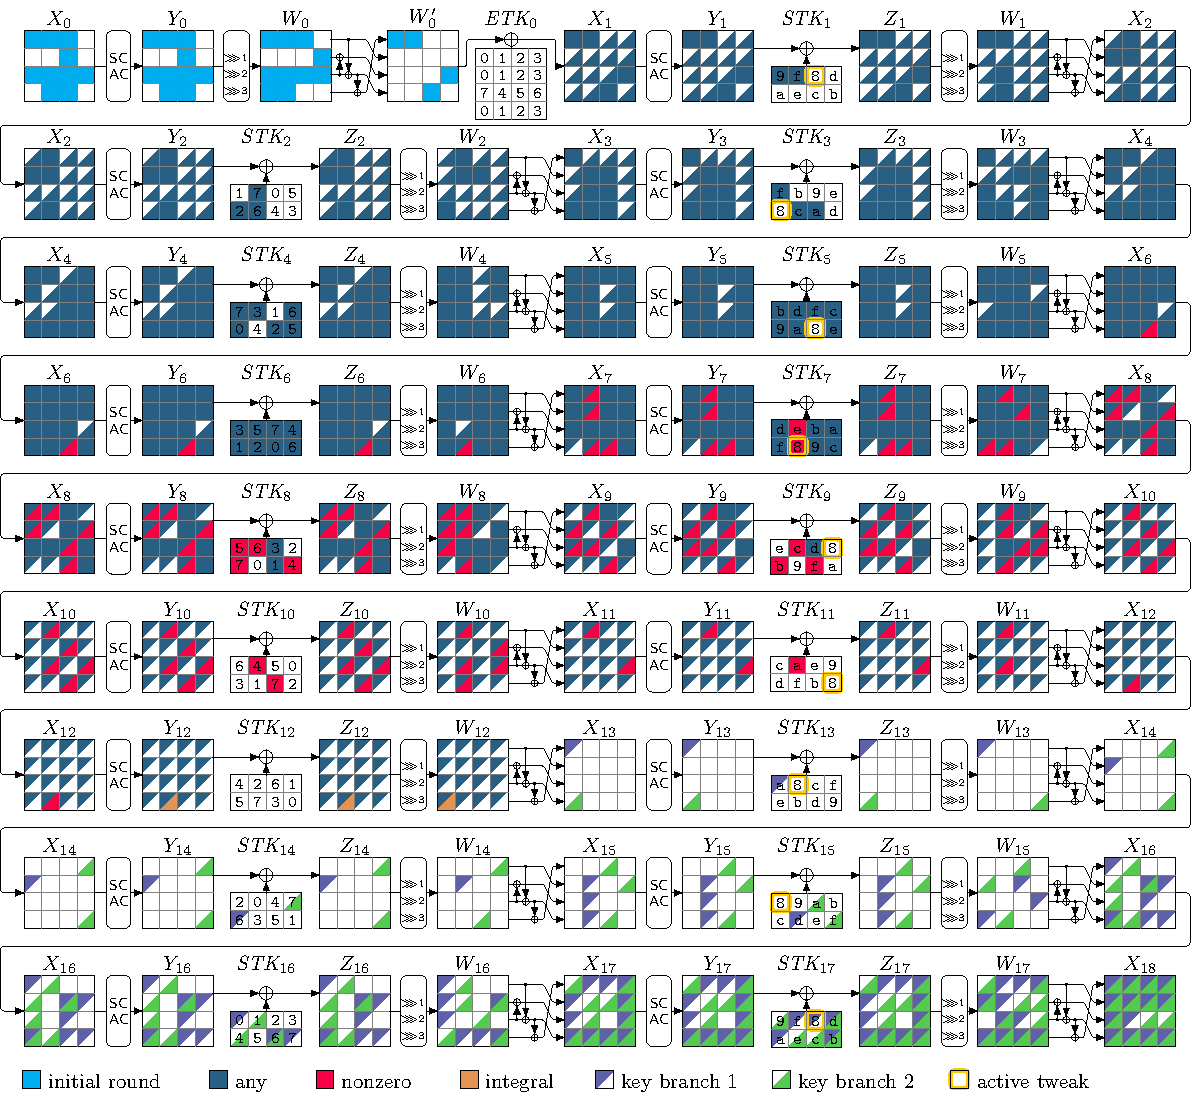
\includegraphics[width=0.95\textwidth]{./figures/zc_rt_skinny_tk1_18r.pdf}
\end{figure}
\column[c]{0.5\textwidth}
\begin{center}
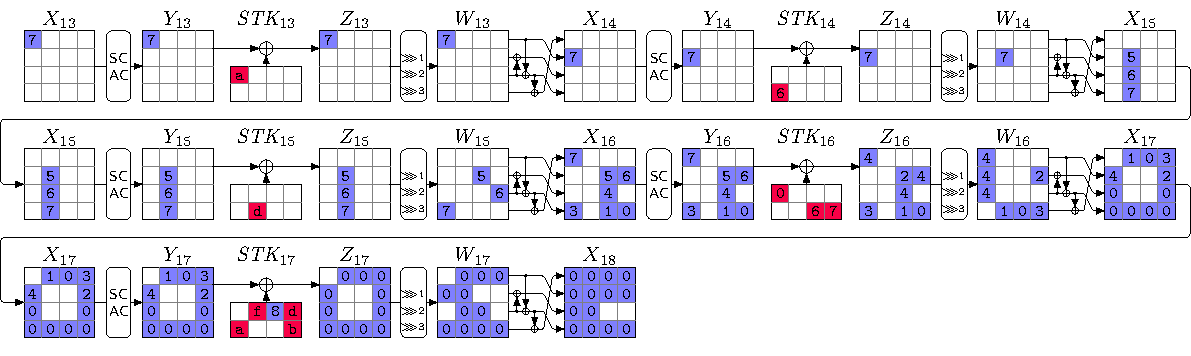
\includegraphics[width=\textwidth]{./figures/zc_rt_skinny_tk1_18r_keyrec1.pdf}
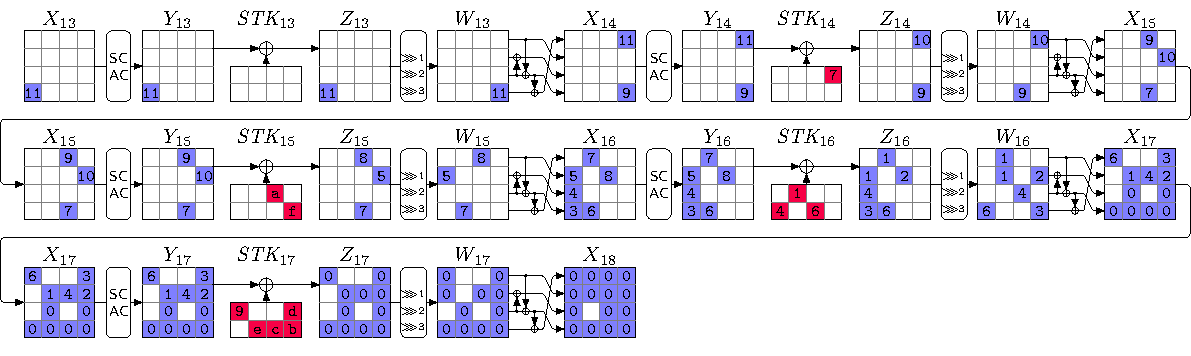
\includegraphics[width=\textwidth]{./figures/zc_rt_skinny_tk1_18r_keyrec2.pdf}
\end{center}
\end{columns}
\end{frame}

%%%%%%%%%%%%%%%%%%%%%%%%%%%%%%%%%%%%%%%%%%%%%%%%%%%%%%%%%%%%%%%%%%%%%%%%%%%%%%%
%%%%%%%%%%%%%%%%%%%%%%%%%%%%%%%%%%%%%%%%%%%%%%%%%%%%%%%%%%%%%%%%%%%%%%%%%%%%%%%
\section{Contributions and Future Works}
\sectionheader[\huge\color{tug}\faHourglassEnd]{Contributions and Future Works}

%%%%%%%%%%%%%%%%%%%%%%%%%%%%%%%%%%%%%%%%%%%%%%%%%%%%%%%%%%%%%%%%%%%%%%%%%%%%%%%
\begin{frame}{Contributions and Future Works}
\vspace{-0.95cm}
\begin{itemize}
\item Contributions
\vspace{-0.3cm}
\begin{itemize}
\small
\item[\textcolor{tugblue}{\faChevronCircleRight}] Improving unified models for finding complete ID/ZC/integral attacks
\item[\textcolor{tugblue}{\faChevronCircleRight}] Introducing a CP model for the partial-sum technique for the first time
\item[\textcolor{tugblue}{\faChevronCircleRight}] Found improved attacks for \cipher{SKINNY}, and \cipher{ForskSKINNY}, and \cipher{QARMAv2}
\end{itemize}
\vspace{-0.3cm}
\item Future works
\vspace{-0.3cm}
\begin{itemize}
\small
\item[\faRoad] Extending our distinguisher models for ID/ZC to find indirect contradictions
\item[\faRoad] Extending our tools to AndRX and ARX ciphers, e.g., \cipher{Simeck}, and \cipher{SPECK}. 
\item[\faRoad] Extending our approach to division property or monomial prediction techniques
\item[\faRoad] Improving the key-recovery part of our CP models for ZC attacks
\end{itemize} 
\end{itemize}
\begin{center}
\vspace{0.10cm}

% {\large Thanks for your attention!}

% \vspace{0.3cm}
\sparen
\faGithub: \url{https://github.com/hadipourh/zeroplus}\\
\vspace{0.1cm}
\faArchive: \url{https://ia.cr/2023/1701}
\end{center}
\end{frame}

















%%%%%%%%%%%%%%%%%%%%%%%%%%%%%%%%%%%%%%%%%%%%%%%%%%%%%%%%%%%%%%%%%%%%%%%%%%%%

\begin{frame}[allowframebreaks]{Bibliography}
  \printbibliography
\end{frame}

%%%%%%%%%%%%%%%%%%%%%%%%%%%%%%%%%%%%%%%%%%%%%%%%%%%%%%%%%%%%%%%%%%%%%%%%%%%%

\begin{filecontents*}[overwrite]{\jobname.bib}
% impossible differential Biham (miss-in-the-middle technique)
@inproceedings{eurocrypt_BihamBS99,
  author    = {Eli Biham and
               Alex Biryukov and
               Adi Shamir},
  title     = {Cryptanalysis of Skipjack Reduced to 31 Rounds Using Impossible Differentials},
  booktitle = {{EUROCRYPT} 1999},
  series    = {LNCS},
  volume    = {1592},
  pages     = {12--23},
  publisher = {Springer},
  year      = {1999},
  doi       = {10.1007/3-540-48910-X_2}
}

% impossible differential Knudesen
@article{knudsen1998deal,
  title     = {DEAL-a 128-bit block cipher},
  author    = {Knudsen, Lars},
  journal   = {complexity},
  volume    = {258},
  number    = {2},
  pages     = {216},
  year      = {1998},
  publisher = {Citeseer}
}

% milp-based method to search for ID attacks - works for ARX and SPN
@misc{eprint_Cui,
  author    = {Tingting Cui and 
            Shiyao Chen and 
            Keting Jia and 
            Kai Fu and 
            Meiqin Wang},
  title     = {New Automatic Search Tool for Impossible Differentials and Zero-Correlation Linear Approximations},
  howpublished = {IACR Cryptology ePrint Archive, Report 2016/689},
  year      = {2016},
  url       = {https://eprint.iacr.org/2016/689}
}

% milp-based method to search for ID attacks - works for SPN
@inproceedings{eurocrypt_SasakiTodo2017,
  author    = {Sasaki, Yu and 
               Todo, Yosuke},              
  Xeditor    = {Coron, Jean-S{\'e}bastien
                and 
                Nielsen, Jesper Buus},
  title     = {New Impossible Differential Search Tool from Design and Cryptanalysis Aspects},
  Xbooktitle = {Advances in Cryptology -- EUROCRYPT 2017},
  booktitle = {{EUROCRYPT} 2017},
  year      = {2017},
  publisher = {Springer International Publishing},
  address   = {Cham},
  pages     = {185--215},
  doi       = {10.1007/978-3-319-56617-7_7}
}

% cp-based method by sun and gerault
@article{tosc_SunGLYTQH2017,
author      = {Sun, Siwei and 
            Gerault, David and 
            Lafourcade, Pascal and 
            Yang, Qianqian and 
            Todo, Yosuke and 
            Qiao, Kexin and 
            Hu, Lei}, 
  title     = {Analysis of {AES}, {SKINNY}, and Others with Constraint Programming}, 
  volume    = {2017}, 
  doi       = {10.13154/tosc.v2017.i1.281-306}, 
  number    = {1}, 
  journal   = {IACR Transactions on Symmetric Cryptology}, 
  year      = {2017}, 
  month     = {Mar.}, 
  pages     = {281–306} 
}

% patrick's tool for mitm and id attacks
@inproceedings{crypto_DerbezF16,
  author    = {Patrick Derbez and
               Pierre-Alain Fouque},
  title     = {Automatic Search of Meet-in-the-Middle and Impossible Differential
               Attacks},
  booktitle = {{CRYPTO} 2016},
  series    = {LNCS},
  volume    = {9815},
  pages     = {157--184},
  publisher = {Springer},
  year      = {2016}
}

% milp model of division 
@inproceedings{asiacrypt_XiangZBL16,
  author    = {Zejun Xiang and
               Wentao Zhang and
               Zhenzhen Bao and
               Dongdai Lin},
  title     = {Applying {MILP} Method to Searching Integral Distinguishers Based
               on Division Property for 6 Lightweight Block Ciphers},
  booktitle = {{ASIACRYPT} 2016},
  series    = {LNCS},
  volume    = {10031},
  pages     = {648--678},
  year      = {2016},
  doi       = {10.1007/978-3-662-53887-6_24}
}

% cp model to encode the deterministic truncated trails
@article{tosc_SunGWW2020, 
  author    = {Sun, Ling and Gerault, David and Wang, Wei and Wang, Meiqin},
  title     = {On the Usage of Deterministic (Related-Key) Truncated Differentials and Multidimensional Linear Approximations for SPN Ciphers}, 
  volume    = {2020},   
  doi       = {10.13154/tosc.v2020.i3.262-287}, 
  number    = {3}, 
  journal   = {IACR Transactions on Symmetric Cryptology}, 
  year      = {2020}, 
  month     = {Sep.}, 
  pages     = {262–287}
}

% blns2018
@article{joc_BouraLNS2018,
  author    = {Boura, Christina and 
               Lallemand, Virginie and 
               Naya-Plasencia, Mar{\'\i}a and 
               Suder, Valentin},
  title     = {Making the impossible possible},
  journal   = {Journal of Cryptology},
  volume    = {31},
  number    = {1},
  pages     = {101--133},
  year      = {2018},
  publisher = {Springer},
  doi       = {10.1007/s00145-016-9251-7}
}

% bns2014
@inproceedings{asiacrypt_BouraNS2014,
  author    = {Boura, Christina and 
               Naya-Plasencia, Maria and 
               Suder, Valentin},
  title     = {Scrutinizing and improving impossible differential attacks: applications to CLEFIA, Camellia, LBlock and Simon},
  booktitle = {International Conference on the Theory and Application of Cryptology and Information Security},
  pages     = {179--199},
  year      = {2014},
  organization = {Springer},
  doi       = {10.1007/978-3-662-45611-8_10}
}

% MiniZinc
@inproceedings{cp_NethercoteSBBDT07,
  author    = {Nicholas Nethercote and
               Peter J. Stuckey and
               Ralph Becket and
               Sebastian Brand and
               Gregory J. Duck and
               Guido Tack},
  title     = {MiniZinc: Towards a Standard {CP} Modelling Language},
  booktitle = {{CP} 2007},
  series    = {LNCS},
  volume    = {4741},
  pages     = {529--543},
  publisher = {Springer},
  year      = {2007}
}

@misc{gurobi,
  author    = {{Gurobi Optimization, LLC}},
  title     = {{Gurobi Optimizer Reference Manual}},
  year      = {2022},
  url       = {https://www.gurobi.com}
}

% Or-Tools
@software{ortools,
  author    = {Laurent Perron and Vincent Furnon},
  title     = {{OR-Tools}},
  version   = {9.3},
  organization = {Google},
  url       = {https://developers.google.com/optimization/},
  date      = {2022-3-15}
}

% seminal paper of ZC attack
@article{dcc_BogdanovR14,
  author    = {Andrey Bogdanov and
               Vincent Rijmen},
  title     = {Linear hulls with correlation zero and linear cryptanalysis of block
               ciphers},
  journal   = {Des. Codes Cryptogr.},
  volume    = {70},
  number    = {3},
  pages     = {369--383},
  year      = {2014},
  doi       = {10.1007/s10623-012-9697-z}
}

% multidimensional zc and link between zc and integral attacks
@inproceedings{asiacrypt_BogdanovLNW12,
  author    = {Andrey Bogdanov and
               Gregor Leander and
               Kaisa Nyberg and
               Meiqin Wang},
  title     = {Integral and Multidimensional Linear Distinguishers with Correlation
               Zero},
  booktitle = {{ASIACRYPT} 2012},
  series    = {LNCS},
  volume    = {7658},
  pages     = {244--261},
  publisher = {Springer},
  year      = {2012},
  doi       = {10.1007/978-3-642-34961-4_16}
}

% link between ZC, ID and Integral attacks
@inproceedings{crypto_SunLRLCWAL15,
  author    = {Bing Sun and
               Zhiqiang Liu and
               Vincent Rijmen and
               Ruilin Li and
               Lei Cheng and
               Qingju Wang and
               Hoda AlKhzaimi and
               Chao Li},
  title     = {Links Among Impossible Differential, Integral and Zero Correlation
               Linear Cryptanalysis},
  booktitle = {{CRYPTO} 2015},
  series    = {LNCS},
  volume    = {9215},
  pages     = {95--115},
  publisher = {Springer},
  year      = {2015},
  doi       = {10.1007/978-3-662-47989-6_5}
}

% zc-integral attack
@article{tosc_AnkeleDGLGY2019, 
  author    = {Ankele, Ralph and Dobraunig, Christoph and Guo, Jian and Lambooij, Eran and Leander, Gregor and Todo, Yosuke}, 
  title     = {Zero-Correlation Attacks on Tweakable Block Ciphers with Linear Tweakey Expansion}, 
  volume    = {2019},
  doi       = {10.13154/tosc.v2019.i1.192-235}, 
  number    = {1}, 
  journal   = {IACR Transactions on Symmetric Cryptology}, 
  year      = {2019},
  month     = {Mar.}, 
  pages     = {192–235},
}

% ID-RT and ZC-ST attacks on SKINNY (Sadeghi et al.)
@article{tosc_SadeghiMB18,
  author    = {Sadegh Sadeghi and
               Tahereh Mohammadi and
               Nasour Bagheri},
  title     = {Cryptanalysis of Reduced round {SKINNY} Block Cipher},
  journal   = {{IACR} Trans. Symmetric Cryptol.},
  volume    = {2018},
  number    = {3},
  pages     = {124--162},
  year      = {2018},
  doi       = {10.13154/tosc.v2018.i3.124-162}
}

% ID attacks on SKINNY in the ST setting (IET)
@article{iet_YangQC17,
  author    = {Dong Yang and
               Wen{-}Feng Qi and
               Hua{-}Jin Chen},
  title     = {Impossible differential attacks on the {SKINNY} family of block ciphers},
  journal   = {{IET} Inf. Secur.},
  volume    = {11},
  number    = {6},
  pages     = {377--385},
  year      = {2017},
  doi       = {10.1049/iet-ifs.2016.0488}
}

% ID attack on SKINNY in the RT setting (ToSC)
@article{journals_tosc_LiuGL17,
  author    = {Guozhen Liu and
               Mohona Ghosh and
               Ling Song},
  title     = {Security Analysis of {SKINNY} under Related-Tweakey Settings},
  journal   = {{IACR} Trans. Symmetric Cryptol.},
  volume    = {2017},
  number    = {3},
  pages     = {37--72},
  year      = {2017},
  doi       = {10.13154/tosc.v2017.i3.37-72}
}

% ID attack on SKINNY (Tolba) WRONG RESULTS!
@inproceedings{africacrypt_Tolba0Y17,
  author    = {Mohamed Tolba and
               Ahmed Abdelkhalek and
               Amr M. Youssef},
  title     = {Impossible Differential Cryptanalysis of Reduced-Round {SKINNY}},
  booktitle = {{AFRICACRYPT} 2017},
  series    = {LNCS},
  volume    = {10239},
  pages     = {117--134},
  year      = {2017},
  doi       = {10.1007/978-3-319-57339-7_7}
}

@article{Zhang2022,
  author    = {Zhang, Yi and
               Cui, Ting and
               Wang, Congjun},
  title     = {{Zero-correlation} linear attack on reduced-round {SKINNY}},
  journal   = {Frontiers of Computer Science},
  volume    = {17},
  number    = {174808 (2023)},
  pages     = {377--385},
  year      = {2022},
  doi       = {10.1007/s11704-022-2206-2}
}

% skinny specification
@inproceedings{skinny,  
  author    = {Beierle, Christof and 
              Jean, J{\'e}r{\'e}my and 
              K{\"o}lbl, Stefan and 
              Leander, Gregor and 
              Moradi, Amir and 
              Peyrin, Thomas and 
              Sasaki, Yu and 
              Sasdrich, Pascal and 
              Sim, Siang Meng},
  title     = {{The SKINNY family of block ciphers and its low-latency variant MANTIS}},
  Xbooktitle= {Advances in Cryptology -- CRYPTO 2016},
  booktitle = {{CRYPTO} 2016},
  pages     = {123--153},
  year      = {2016},
  organization= {Springer},
  doi       = {10.1007/978-3-662-53008-5_5},
}

% QARMAv2 block cipher
@article{cryptoeprint_qarmav2,
  author       = {Roberto Avanzi and
                  Subhadeep Banik and
                  Orr Dunkelman and
                  Maria Eichlseder and
                  Shibam Ghosh and
                  Marcel Nageler and
                  Francesco Regazzoni},
  title        = {The {QARMAv2} Family of Tweakable Block Ciphers},
  journal      = {{IACR} Trans. Symmetric Cryptol.},
  volume       = {2023},
  number       = {3},
  pages        = {25--73},
  year         = {2023},
  doi          = {10.46586/TOSC.V2023.I3.25-73},
}

% related key zc/integral
@inproceedings{ctrsa_NiuLSW21,
  author    = {Chao Niu and
               Muzhou Li and
               Siwei Sun and
               Meiqin Wang},
  title     = {Zero-Correlation Linear Cryptanalysis with Equal Treatment for Plaintexts
               and Tweakeys},
  booktitle = {{CT-RSA} 2021},
  series    = {LNCS},
  volume    = {12704},
  pages     = {126--147},
  publisher = {Springer},
  year      = {2021},
  doi       = {10.1007/978-3-030-75539-3_6}
}

% Our EUROCRYPT 2023 paper
@inproceedings{eurocrypt_HadipourSE23,
  author       = {Hosein Hadipour and
                  Sadegh Sadeghi and
                  Maria Eichlseder},
  title        = {Finding the Impossible: Automated Search for Full Impossible Differential,
                  Zero-Correlation, and Integral Attacks},
  booktitle    = {{EUROCRYPT} 2023},
  series       = {LNCS},
  volume       = {14007},
  pages        = {128--157},
  publisher    = {Springer},
  year         = {2023},
  doi          = {10.1007/978-3-031-30634-1_5}
}

% ForkCipher Cryptanalysis
@article{tosc_BariantDL20,
  author       = {Augustin Bariant and
                  Nicolas David and
                  Ga{\"{e}}tan Leurent},
  title        = {Cryptanalysis of {Forkciphers}},
  journal      = {{IACR} Trans. Symmetric Cryptol.},
  volume       = {2020},
  number       = {1},
  pages        = {233--265},
  year         = {2020},
  doi          = {10.13154/tosc.v2020.i1.233-265}
}

% One of the seminal papers for integral attacks
@incollection{hod_discrete_derivatives_lai1994higher,
  author    = {Lai, Xuejia},
  title     = {Higher order derivatives and differential cryptanalysis},
  booktitle = {Communications and cryptography},
  pages     = {227--233},
  year      = {1994},
  publisher = {Springer}
}

% One of the seminal papers for integral attacks
@inproceedings{square_fse_DaemenKR97,
  author    = {Joan Daemen and
               Lars R. Knudsen and
               Vincent Rijmen},
  title     = {The Block Cipher {Square}},
  booktitle = {{FSE} 1997},
  series    = {LNCS},
  volume    = {1267},
  pages     = {149--165},
  publisher = {Springer},
  year      = {1997},
  doi       = {10.1007/BFb0052343},
}

% the early abort tehnique
@inproceedings{ctrsa_LuKKD08,
  author    = {Jiqiang Lu and
               Jongsung Kim and
               Nathan Keller and
               Orr Dunkelman},
  title     = {Improving the Efficiency of Impossible Differential Cryptanalysis
               of Reduced {Camellia} and {MISTY1}},
  booktitle = {{CT-RSA} 2008},
  series    = {LNCS},
  volume    = {4964},
  pages     = {370--386},
  publisher = {Springer},
  year      = {2008},
  doi          = {10.1007/978-3-540-79263-5_24},
}

% partial sum technique
@inproceedings{fseFergusonKLSSWW00,
  author    = {Niels Ferguson and
               John Kelsey and
               Stefan Lucks and
               Bruce Schneier and
               Michael Stay and
               David A. Wagner and
               Doug Whiting},
  Xeditor   = {Bruce Schneier},
  title     = {Improved Cryptanalysis of {Rijndael}},
  booktitle = {{FSE} 2000},
  series    = {LNCS},
  volume    = {1978},
  pages     = {213--230},
  publisher = {Springer},
  year      = {2000},
  doi       = {10.1007/3-540-44706-7_15},
}

% The seminal paper for undisrupted bits
@article{journals_jcam_Tezcan14_ubits,
  author       = {Cihangir Tezcan},
  title        = {Improbable differential attacks on {Present} using undisturbed bits},
  journal      = {J. Comput. Appl. Math.},
  volume       = {259},
  pages        = {503--511},
  year         = {2014},
  doi          = {10.1016/j.cam.2013.06.023}
}

\end{filecontents*}

\end{document}
